\documentclass[11pt]{beamer}
\usetheme{Luebeck}
%\usecolortheme{seahorse}
\useinnertheme{rectangles}
\useoutertheme{infolines}
\usepackage{xcolor}
\usepackage{natbib}
\usepackage[utf8]{inputenc}
\usepackage{tikz}
\usepackage{tabularx}
\usepackage{lipsum}
\usepackage{amsmath,graphicx,dsfont}
\usepackage{amssymb}
\usepackage{graphicx}
\usepackage{multirow}
\usetikzlibrary{shapes,backgrounds,arrows,automata,snakes,shadows,positioning, mindmap}
%\usepackage[citestyle=verbose]{biblatex}
%===================================
\newcommand\G{\mathcal{G}}
\newcommand\J{\mathcal{J}}
\newcommand{\Esp}{{\mathds{E}}}
\DeclareMathOperator*{\Cov}{\mathbb{C}\text{ov}}
% Notations tilde
\newcommand\Pt{\widetilde{P}}
\newcommand\pt{\widetilde{p}}
\newcommand\et{\widetilde{\mathds{E}}}
\newcommand\e{{\mathds{E}}}
\newcommand{\betabft}{{\widetilde{\betabf}}}
\newcommand{\Mbft}{{\widetilde{\Mbf}}}
\newcommand{\Sbft}{{\widetilde{\Sbf}}}
\newcommand\mt{\widetilde{m}}
\newcommand\St{\widetilde{S}}
\newcommand\mbt{\widetilde{\bf m}}
\newcommand\Sbt{\widetilde{\bf S}}
\newcommand{\betat}{{\widetilde{\beta}}}
\newcommand{\Bt}{{\widetilde{B}}}

% Notations bf
\newcommand\gammab{{\boldsymbol{\gamma}}}
\newcommand\betab{{\boldsymbol{\beta}}}
\newcommand\thetab{{\boldsymbol{\theta}}}
\newcommand\lambdab{{\boldsymbol{\lambda}}}
\newcommand\Lambdab{{\boldsymbol{\Lambda}}}
\newcommand\Sigmab{{\boldsymbol{\Sigma}}}
\newcommand\Omegab{{\boldsymbol{\Omega}}}
\newcommand\cst{\text{cst}}
\newcommand\Ob{{\bf O}}
\newcommand\Hb{{\boldsymbol{H}}}
\newcommand\Mbf{{\bf M}}
\newcommand\Qbf{{\bf Q}}
\newcommand\Abf{{\bf A}}
\newcommand\Wbf{{\bf W}}
\newcommand\Mb{{\boldsymbol{M}}}
\newcommand\Qb{{\bf Q}}
\newcommand\Wb{{\bf W}}
\newcommand\Xb{{\bf X}}
\newcommand\xb{{\boldsymbol{x}}}
\newcommand\Yb{{\bf Y}}
\newcommand\Zb{{\bf Z}}
\newcommand\Gb{{\bf G}}
\newcommand\zb{{\boldsymbol{z}}}
\newcommand\yb{{\boldsymbol{y}}}
\newcommand\Ibb{\mathbb{I}}
\newcommand{\betabf}{{\boldsymbol{\beta}}}
\newcommand{\thetabf}{{\boldsymbol{\theta}}}
\newcommand{\sigmabf}{{\boldsymbol{\sigma}}}
\newcommand{\Omegabf}{{\boldsymbol{\Omega}}}
\newcommand{\Sigmabf}{{\boldsymbol{\Sigma}}}
\newcommand{\Gammabf}{{\boldsymbol{\Gamma}}}
\newcommand{\zerobf}{{\boldsymbol{0}}}
\newcommand{\Xbf}{{\boldsymbol{X}}}
\newcommand{\xbf}{{\boldsymbol{x}}}
\newcommand{\Ybf}{{\boldsymbol{Y}}}
\newcommand{\Zbf}{{\boldsymbol{Z}}}
\newcommand{\hbf}{{\boldsymbol{h}}}
\newcommand{\Hbf}{{\boldsymbol{H}}}
\newcommand{\Ubf}{{\boldsymbol{U}}}
%\newcommand{\Mbf}{{\boldsymbol{M}}}
%\newcommand{\Qbf}{{\boldsymbol{Q}}}
\newcommand{\Rbf}{{\boldsymbol{R}}}
\newcommand{\Sbf}{{\boldsymbol{S}}}
\newcommand{\sbf}{{\boldsymbol{s}}}
\newcommand{\mbf}{{\boldsymbol{m}}}

%===================================
\newcommand*\xbar[1]{%
   \hbox{%
     \vbox{%
       \hrule height 0.5pt % The actual bar
       \kern0.5ex%         % Distance between bar and symbol
       \hbox{%
         \kern-0.1em%      % Shortening on the left side
         \ensuremath{#1}%
         \kern-0.1em%      % Shortening on the right side
       }%
     }%
   }%
} 

\newcommand{\Ccal}{\mathcal{C}}
\newcommand{\Pcal}{\mathcal{P}}
\newcommand{\edgeunit}{1.5}
\newcommand{\length}{1.5}
\newcommand{\dist}{6}
\newcommand{\smalledgeunit}{1}
\newcommand{\emphase}[1]{\textcolor{Complement}{#1}}
\newcommand{\bleu}[1]{\textcolor{Framableulight}{#1}}
\newcommand{\pos}[1]{\textcolor{Darkgreen}{#1}}
\newcommand{\nega}[1]{\textcolor{Nicered}{#1}}
\newcommand{\independent}{\perp \!\!\! \perp}

\newcommand{\Ncal}{\mathcal{N}}
\newcommand{\Scal}{\mathcal{S}}
\tikzset{%
    observed/.style={%
    scale=0.6,circle,draw=Framableulight,transform shape,fill=white,font=\Large}
}
\tikzset{%
    bigMissing/.style={%
    scale=0.6,circle,draw=orange,transform shape,fill=white,font=\Large}
}
\tikzset{%
    basic/.style={%
    scale=0.4,circle,draw=Framableu,transform shape,fill=Framableulight,font=\small}
}
\tikzset{%
    large/.style={%
    scale=0.7,circle,draw=white,transform shape,fill=Framableulight,font=\small}
}
\tikzset{%
    missing/.style={%
    scale=0.7,circle,draw=orange,transform shape,fill=orange,font=\small}
}
\tikzset{%
    variable/.style={%
    scale=0.9,rectangle,draw=white,transform shape,fill=white,font=\Large}
}


\newcommand{\argmin}{\mathop{\mathrm{argmin}}}   
\newcommand{\argmax}{\mathop{\mathrm{argmax}}}   
\newcommand{\backupbegin}{
   \newcounter{framenumberappendix}
   \setcounter{framenumberappendix}{\value{framenumber}}
}
\newcommand{\backupend}{
   \addtocounter{framenumberappendix}{-\value{framenumber}}
   \addtocounter{framenumber}{\value{framenumberappendix}} 
}

\makeatletter
\setbeamertemplate{footline}
{
  \leavevmode%
  \hbox{%
  \begin{beamercolorbox}[wd=.333333\paperwidth,ht=2.25ex,dp=1ex,center]{author in head/foot}%
    \usebeamerfont{author in head/foot}Network inference from incomplete data%~~\beamer@ifempty{\insertshortinstitute}{}{(\insertshortinstitute)}
  \end{beamercolorbox}%
  \begin{beamercolorbox}[wd=.333333\paperwidth,ht=2.25ex,dp=1ex,center]{title in head/foot}%
    \usebeamerfont{title in head/foot} PhD defense
  \end{beamercolorbox}%
  \begin{beamercolorbox}[wd=.333333\paperwidth,ht=2.25ex,dp=1ex,right]{date in head/foot}%
    \usebeamerfont{date in head/foot}\insertshortdate{}\hspace*{2em}
    \insertframenumber{} / \inserttotalframenumber\hspace*{2ex} 
  \end{beamercolorbox}}%
  \vskip0pt%
}
\makeatother
%===================================
\definecolor{Framableu}{RGB}{12,91,122}
\definecolor{Framableulight}{RGB}{18,144,176}
\definecolor{Nicered}{RGB}{176,18,65}
%\definecolor{Nicered}{RGB}{141,14,52}
\definecolor{Lightpink}{RGB}{229,177,218}
\definecolor{Green}{RGB}{144,176,18}
\definecolor{Lightcomplement}{RGB}{235,204,196}
\definecolor{Darkgoldenrod}{RGB}{176,144,18}
\definecolor{Darkomplement}{RGB}{122,43,12}
\definecolor{Complement}{RGB}{176,50,18}
\definecolor{Darkgreen}{RGB}{52,141,14}
%===================================
\setbeamertemplate{itemize items}[square]
\setbeamertemplate{blocks}[shadow=false]
\setbeamertemplate{caption}{\raggedright\insertcaption\par}
%===================================
\setbeamercolor{section in head/foot}{fg=white,bg=Framableu}
\setbeamercolor{subsection in head/foot}{fg=white,bg=Framableulight}
\setbeamercolor{author in head/foot}{bg=Framableu}
\setbeamercolor{item}{fg=Framableulight}
\setbeamercolor*{structure}{bg=Framableulight!20,fg=Framableulight}
\setbeamercolor*{palette secondary}{use=structure,fg=white,bg=structure.fg!75}
\setbeamercolor{section in toc}{fg=Framableu,bg=white}
\setbeamercolor{frametitle}{fg=Framableu!80,bg=white}
\setbeamercolor{block title}{fg=white, bg=Framableulight}  
\RequirePackage{hyperref} 
%\hypersetup{colorlinks=true, citecolor=blue, filecolor=black, linkcolor=black, urlcolor=black}
%\hypersetup{
%    bookmarks=true,         % show bookmarks bar?
%    unicode=false,          % non-Latin characters in Acrobat’s bookmarks
%    pdftoolbar=true,        % show Acrobat’s toolbar?
%    pdfmenubar=true,        % show Acrobat’s menu?
%    pdffitwindow=false,     % window fit to page when opened
%    pdfstartview={FitH},    % fits the width of the page to the window
%    pdftitle={Network inference from incomplete abundance data},    % title
%    pdfauthor={Raphaelle Momal},     % author
%    pdfsubject={Applied mathematics},   % subject of the document
%    pdfcreator={Raphaelle Momal},   % creator of the document
%    pdfnewwindow=true,      % links in new PDF window
%    colorlinks=true,       % false: boxed links; true: colored links
%    linkcolor=black,%bleuvertgtis,          % color of internal links (change box color with linkbordercolor)
%    citecolor=black,        % color of links to bibliography
%    filecolor=rosefonce,      % color of file links
%    urlcolor=blue1           % color of external links
%}
 
\definecolor{blue1}{RGB}{55,126,184}
\definecolor{blue2}{RGB}{29,120,166}%49,113,165
%===================================
\title{Inference of species interaction networks from incomplete data}

\author{Raphaëlle Momal\\
\tiny{Supervision:  S. Robin$^{{1}}$ and C. Ambroise$^{\inst{2}}$  }}
\institute[]
{
  \inst{1}%
  UMR AgroParisTech / INRA MIA-Paris \\
  \inst{2}%
  LaMME, Evry
  }
\date{November 12$^{\text{th}}$, 2020}


%%%%%%%%%%%%%%%%%%%%%%%%%%%%%%%%%%
%%%%%%%%%%%%%%%%%%%%%%%%%%%%%%%%%%
%%%%%%%%%%%%%%%%%%%%%%%%%%%%%%%%%%
\begin{document}

\begin{frame}
    \titlepage
    \begin{center}
    
\includegraphics[width=0.15\linewidth]{images/UPsaclay.png}
    
\includegraphics[width=0.2\linewidth]{images/agro.PNG}\hspace{0.1cm}
	
\includegraphics[width=0.15\linewidth]{images/inrae.png}\hspace{0.15cm}
	
\includegraphics[width=0.17\linewidth]{images/lmh.png}\hspace{0.15cm}
\end{center}
\end{frame}

%====================================================================
%====================================================================


\section{Introduction}
\subsection{Biological context}
%=======================================
\begin{frame}{Network example in ecology}
\begin{columns}
\begin{column}{7.5cm}
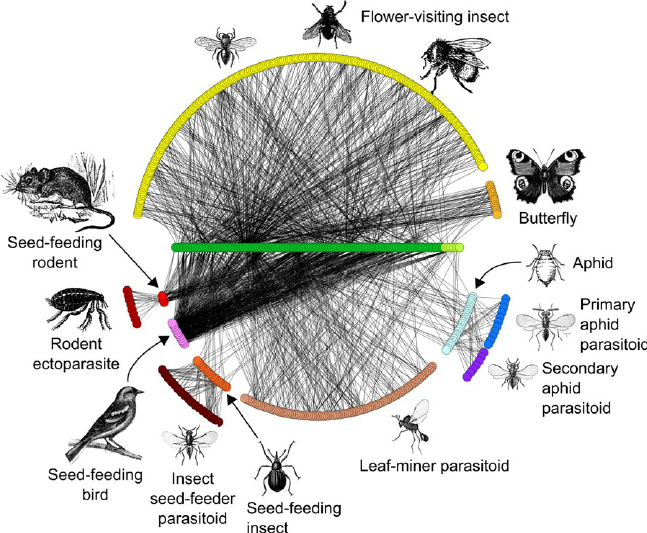
\includegraphics[width=8cm]{images/Species-interaction-networks-at-Norwood-Farm-Somerset-UK-revised-from-Pocock-et-al.png}
\footnotesize{Pocock et. al 2012}
\end{column}
\begin{column}{4.5cm}
\begin{itemize}
    \item Tool to better understand species interactions, eco-systems organizations
    \item Allows for resilience analyses, pathogens control, ecosystem comparison, response prediction...
\end{itemize}
\end{column}
\end{columns}
\end{frame}
\begin{frame}{Species co-occurrence network}
\vspace{-0.5cm}
 \begin{figure}
 \centering
 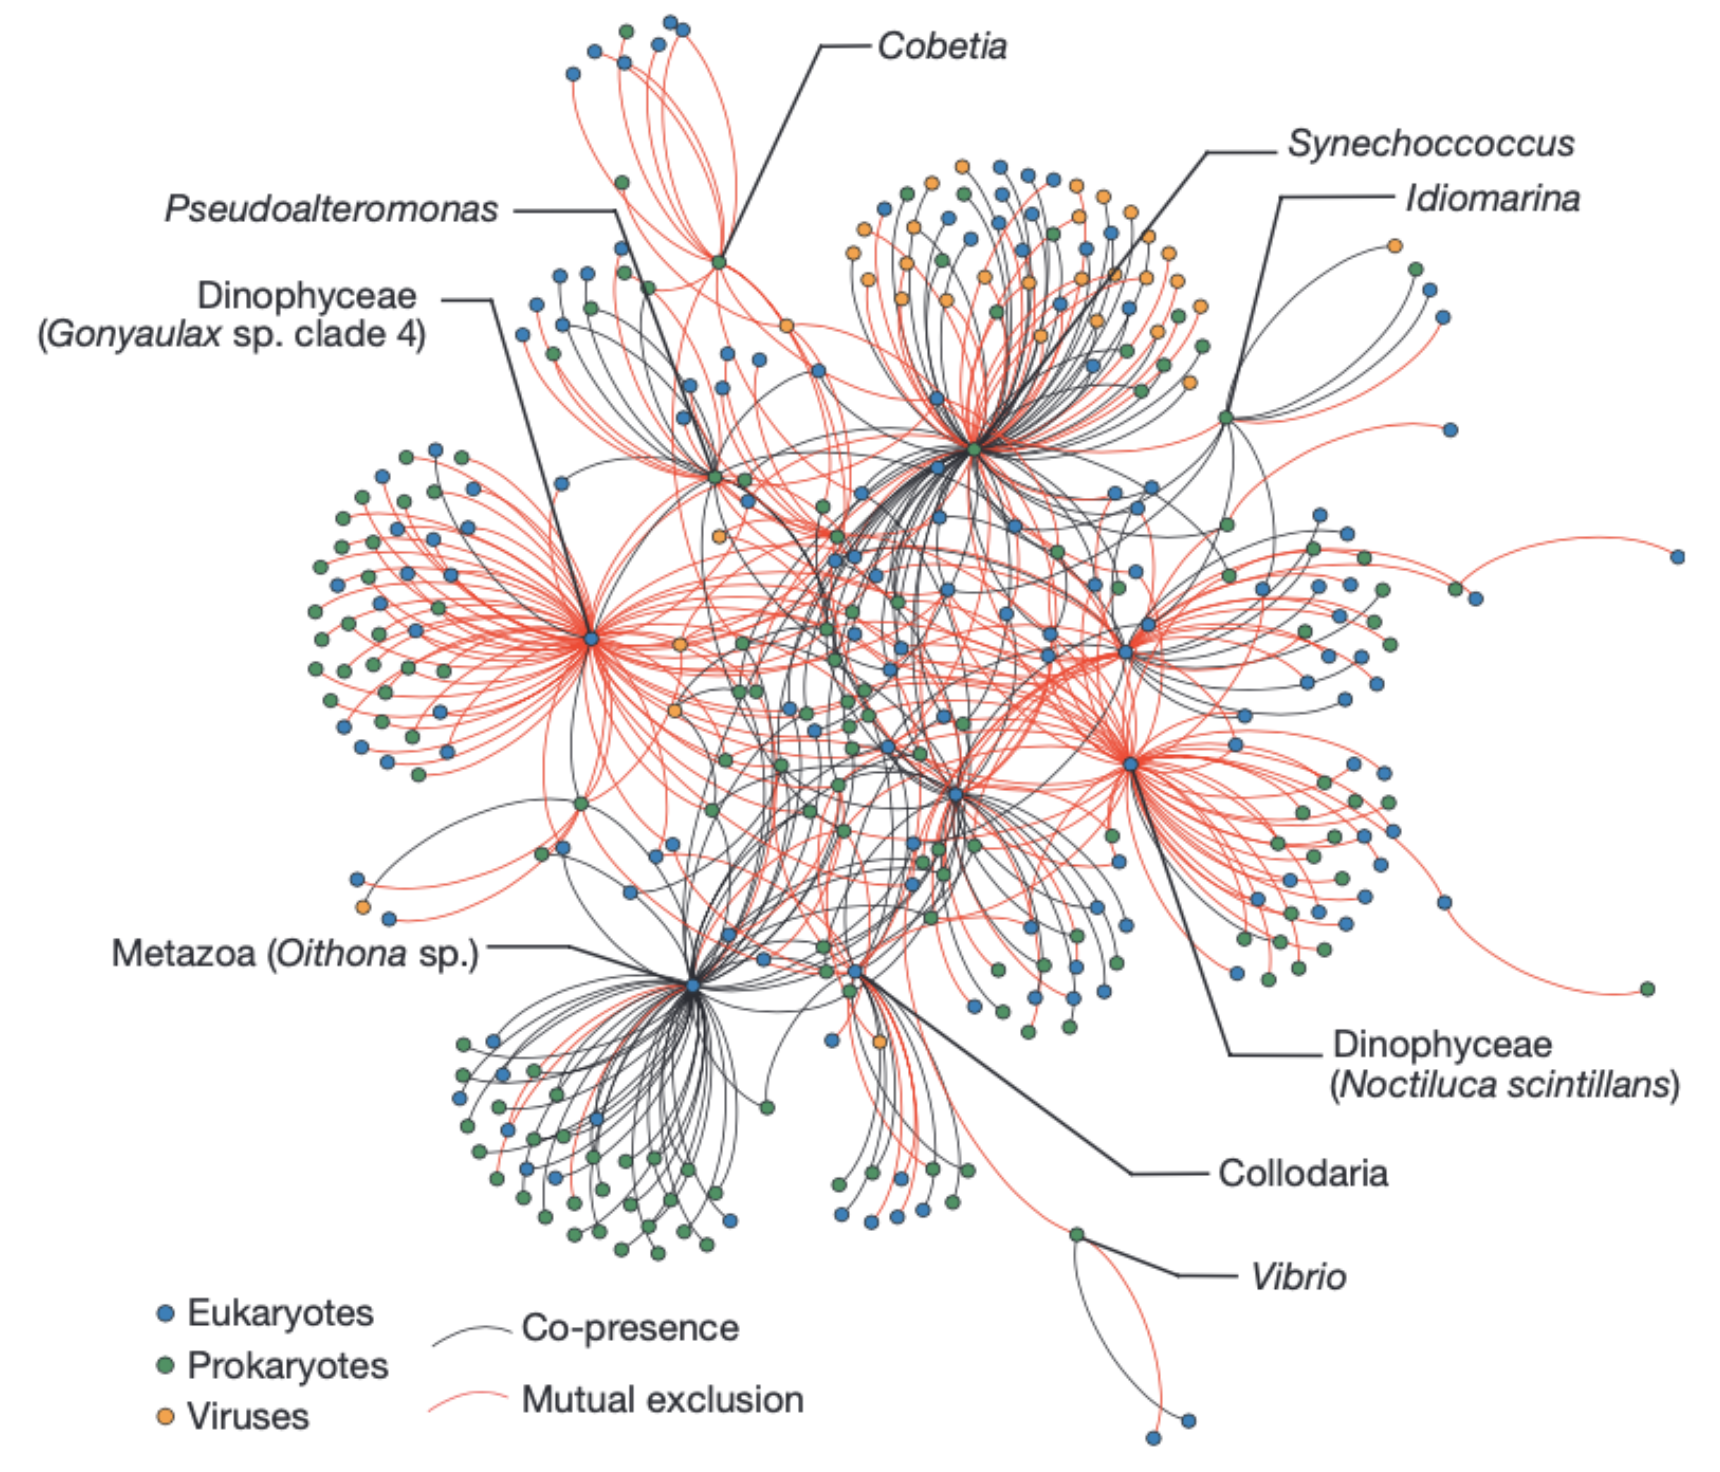
\includegraphics[width=8cm]{images/plancton.png}
\caption{\footnotesize{Integrated plankton community network related to carbon export at 150m (Guidi et. al, 2016)}}

 \end{figure}
 
\end{frame}
\subsection{Links}

\subsection{Problematic}
%=======================================
\begin{frame}{Aim of network inference from abundance data}
 \begin{figure}[H]
   
    \begin{tabular}{llll}
%        $\Xb$ & & $\Yb$ & & $\widehat{G}$ \\
        {\scriptsize{ \begin{tabular}{rrrrr}
EFI & ELA & GDE & GME & HFA \\
%\hline
 71 &   1 &   5 &   6 &   0 \\
118 &   2 &   3 &   0 &   0 \\
 69 &   0 &   6 &   2 &   0 \\
 56 &   0 &   0 &   0 &   0 \\
  0 &   1 &   1 &   0 &   0 \\
  0 &   0 &   2 &   0 &   0 \\
\vdots & \vdots & \vdots & \vdots & \vdots
\end{tabular}
%
%\begin{tabular}{rrrrrrr}
%\dots & EFI & ELA & GDE & GME & HFA & \dots \\
%\hline
%&  71 &   1 &   5 &   6 &   0 & \\
%& 118 &   2 &   3 &   0 &   0 & \\
%&  69 &   0 &   6 &   2 &   0 & \\
%&  56 &   0 &   0 &   0 &   0 & \\
%&   0 &   1 &   1 &   0 &   0 & \\
%&   0 &   0 &   2 &   0 &   0 & \\
%& \vdots & \vdots & \vdots & \vdots & \vdots
%\end{tabular} }} & 
        {\scriptsize{ \begin{tabular}{rr}
date & site \\
%\hline
apr93 & km03 \\
apr93 & km03 \\
apr93 & km03 \\
apr93 & km03 \\
apr93 & km17 \\
apr93 & km17 \\
\vdots & \vdots
\end{tabular} }} &  \hspace{0.05cm} &
        \begin{tabular}{c}
        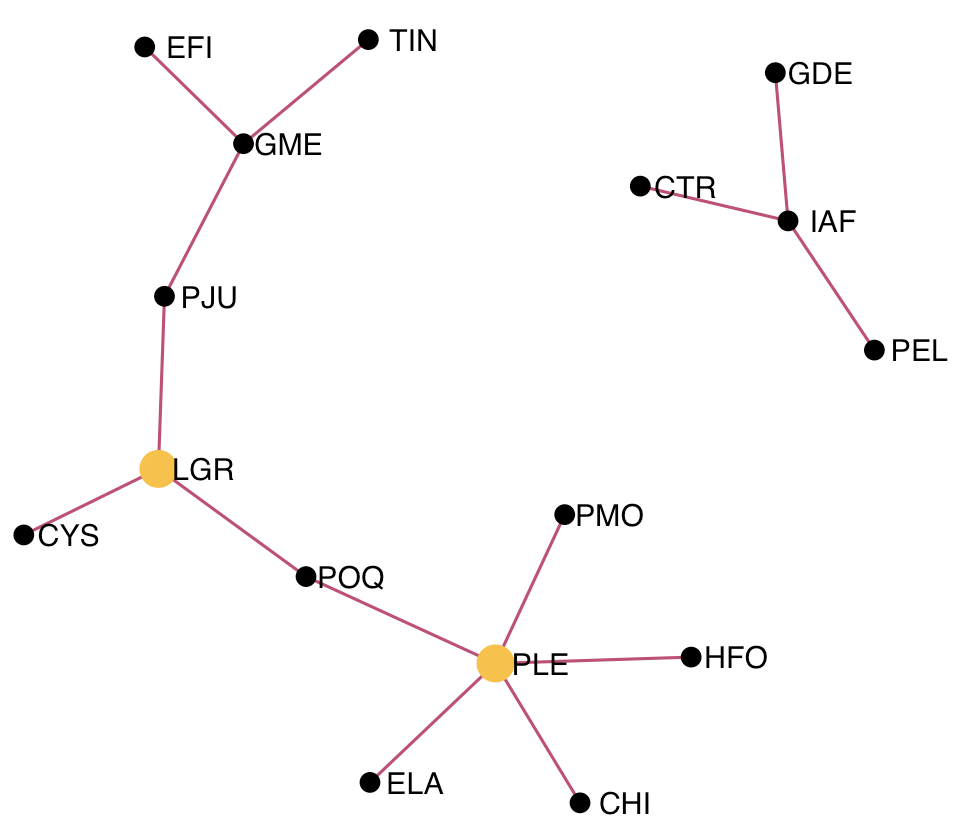
\includegraphics[width=.3\linewidth]{images/barans2plot.png}
        \end{tabular} \\
       ($a$) species abundances  $\bf{Y}$ &($b$) covariates $\bf{X}$ &&($c$) $\Gb$    
    \end{tabular}
    \caption{Data sample from the Fatala river dataset (Baran 1995). }
    \label{fig:networkinference}
\end{figure}
\begin{itemize}
\item Unknown underlying structure.
\item Unobserved interaction data.
\end{itemize}
 
\end{frame}
%=======================================
\begin{frame}{Incomplete data: a missing species/covariate}
\emphase{Marginalization of graphs:}
 \begin{columns} 
 \begin{column}{0.4\linewidth}
 \begin{flushright}
\begin{tabular}{c}
 {Complete graph:}\\\\
 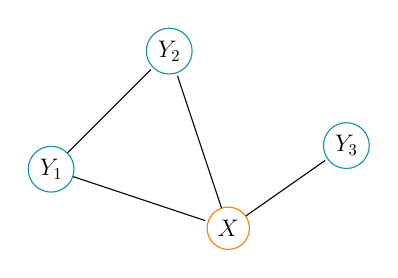
\begin{tikzpicture}
     
      \tikzstyle{every edge}=[-,>=stealth',shorten >=1pt,auto,thin,draw]
		\node[observed] (A1) at (0*\edgeunit, 0*\edgeunit) {$Y_1$};
	\node[bigMissing] (A2) at (1.5*\edgeunit, -0.5*\edgeunit) {
		$X$};
	
		\node[observed] (A3) at (1*\edgeunit, 1*\edgeunit) {$Y_2$};
		\node[observed] (A4) at (2.5*\edgeunit, 0.2*\edgeunit) {$Y_3$};
		\path (A1) edge [] (A2)
        (A1) edge [] (A3)
        (A2) edge [] (A3)
        (A2) edge [] (A4);
\end{tikzpicture}
\end{tabular}\\
 \end{flushright}
 \end{column}
 \begin{column}{0.1\linewidth}
\begin{center}
 $\Longrightarrow$
\end{center}
\end{column}
 \begin{column}{0.4\linewidth}
 \begin{flushleft}
\vspace{0.8cm}
\begin{tabular}{c}
  {Marginal graph}:\\\\
 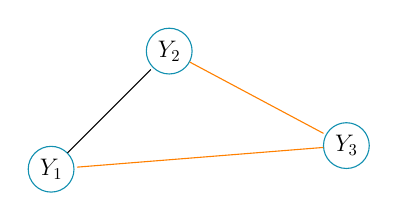
\begin{tikzpicture}
      \tikzstyle{every edge}=[-,>=stealth',shorten >=1pt,auto,thin,draw]
		\node[observed] (A1) at (0*\edgeunit, 0*\edgeunit) {$Y_1$};
		%\node[observed] (A2) at (1.5*\edgeunit, -0.5*\edgeunit) {$A_2$};
		\node[observed] (A3) at (1*\edgeunit, 1*\edgeunit) {$Y_2$};
		\node[observed] (A4) at (2.5*\edgeunit, 0.2*\edgeunit) {$Y_3$};
		\path  (A1) edge [] (A3)
        (A3) edge [orange] (A4)
        (A4) edge [orange] (A1);
\end{tikzpicture}
\end{tabular}\\
\end{flushleft}
Spurious edges leading to wrong interpretation\\
 \end{column}
\end{columns}
\bigskip

$X$ is a \emphase{missing actor}.
\end{frame}
%=======================================
\begin{frame}{Incomplete abundance data}
 \begin{figure}[H]
   
    \begin{tabular}{lllc}
%        $\Xb$ & & $\Yb$ & & $\widehat{G}$ \\
        {\scriptsize{ \begin{tabular}{rrrrr}
EFI & ELA & GDE & {\color[HTML]{9B9B9B} GME}  \\
%\hline
 71 &   1 &   5 &  {\color[HTML]{9B9B9B} 6}       \\
118 &   2 &   3 &  {\color[HTML]{9B9B9B} 0}       \\
 69 &   0 &   6 &   {\color[HTML]{9B9B9B} 2}    \\
 56 &   0 &   0 &  {\color[HTML]{9B9B9B} 0}    \\
  0 &   1 &   1 &   {\color[HTML]{9B9B9B} 0} \\
  0 &   0 &   2 &   {\color[HTML]{9B9B9B} 0}  \\
\vdots & \vdots & \vdots & \vdots  
\end{tabular} }} & 
        {\scriptsize{ \begin{tabular}{rr}
date & {\color[HTML]{9B9B9B} site} \\
%\hline
apr93 &{\color[HTML]{9B9B9B} km03} \\
apr93 & {\color[HTML]{9B9B9B} km03}  \\
apr93 & {\color[HTML]{9B9B9B} km03}  \\
apr93 & {\color[HTML]{9B9B9B} km03}  \\
apr93 & {\color[HTML]{9B9B9B} km17}  \\
apr93 & {\color[HTML]{9B9B9B} km17}  \\
\vdots & \vdots
\end{tabular} }} &  $\Longrightarrow$ &
        \begin{tabular}{c}
       \emphase{\LARGE{?}}
        \end{tabular} \\
       ($a$) incomplete abundances  $\bf{Y}$ &($b$) incomplete $\bf{X}$ &&($c$) \emphase{complete} $\Gb$   
    \end{tabular}
 
\end{figure}
\bigskip 

%\begin{center}
%What happens if some data are unobserved?
%\end{center}

\end{frame}
%=======================================

\section{Mathematical framework}
%=======================================

\begin{frame}{}
\begin{center}
\Huge{\bleu{Mathematical framework}}
\end{center}
\normalsize
\begin{center}
\begin{description}
\item[i] {Graphical Models}
\item[ii]  Graph exploration with trees
\item[iii]  Poisson log-Normal model
\end{description}
\end{center}

\end{frame}

 \subsection{Graphical Models}
  %=======================================
\begin{frame}{Which statistical link?}
\begin{columns}
\begin{column}{0.5\linewidth}
\begin{center}
Dependence? \vspace{1cm}

\begin{tikzpicture}	
      \tikzstyle{every edge}=[-,>=stealth',shorten >=1pt,auto,thin,draw]
		\node[] (A1) at (0*\edgeunit, 0*\edgeunit) {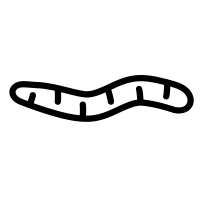
\includegraphics[width=1cm]{images/worm.png}};
		\node[] (A2) at (1*\edgeunit, 1.5*\edgeunit) {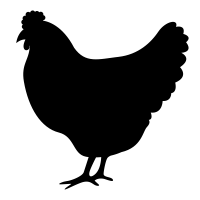
\includegraphics[width=1cm]{images/chick.png}};
		\node[] (A3) at (2.2*\edgeunit, 0*\edgeunit) {
\includegraphics[width=1.5cm]{images/fox.png}};
		\path (A1) edge [] (A2)
        (A1) edge [] (A3)
        (A2) edge [] (A3);
	\onslide<2->
		\node[] (A4) at (1.1*\edgeunit, -1*\edgeunit) {\text{Spurious dependence}};
	   \node[Complement] (A5) at (1.1*\edgeunit,0){$\Large\boldsymbol{\times}$};
      	\path   (A4) edge [->] (A5);
\end{tikzpicture}  
\end{center}
	\end{column}
	\begin{column}{0.5\linewidth}
	\onslide<2>{
	\emphase{Conditional dependence:\\}
	\begin{itemize}
	\item Only direct links: less links.
	\item Probabilistic background\\$p(a,b\mid c) = p(a\mid c)\, p(b \mid c)$.
	\item Possible to model.
	\end{itemize}}
	\end{column}
	\end{columns}
\end{frame}
  %=======================================
 \begin{frame}{Graphical Models}
 \begin{columns}
 \begin{column}{0.4\linewidth}
  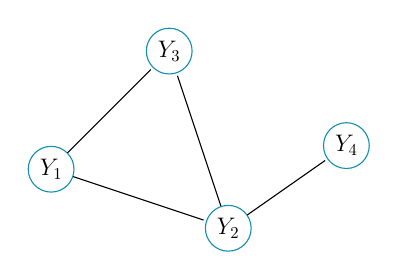
\begin{tikzpicture}
      \tikzstyle{every edge}=[-,>=stealth',shorten >=1pt,auto,thin,draw]
		\node[observed] (A1) at (0*\edgeunit, 0*\edgeunit) {$Y_1$};
	\node[observed] (A2) at (1.5*\edgeunit, -0.5*\edgeunit) {$Y_2$};
		\node[observed] (A3) at (1*\edgeunit, 1*\edgeunit) {$Y_3$};
		\node[observed] (A4) at (2.5*\edgeunit, 0.2*\edgeunit) {$Y_4$};
		\path (A1) edge [] (A2)
        (A1) edge [] (A3)
        (A2) edge [] (A3)
        (A2) edge [] (A4);
\end{tikzpicture}
 \end{column}
  \begin{column}{0.6\linewidth}
\bleu{Global Markov:}\\
  $ Y_2 \text{ separates } Y_3 \text{ from } Y_4  \Rightarrow Y_3\independent Y_4 \mid Y_2.$
  \bigskip
   \bigskip
   
 \bleu{Hammersley-Clifford:}\\
Strictly positive and {continuous} density $f$:
$ f\text{ global Markov} \iff \displaystyle f(\Ybf) = \prod_{c\in \mathcal{C} }\psi(Y_c).$
 \end{column}
  \end{columns}
  \bigskip
  
Here $\mathcal{C} =\big\{\{1, 2, 3\},\{2, 4\}\big\}$:
$$f(\Ybf) = \psi(Y_1,Y_2,Y_3)\times \psi(Y_2,Y_4)$$

 \end{frame}
 %=======================================
\begin{frame}{Marginalization of graphs}
 \begin{columns} 
 \begin{column}{0.4\linewidth}
 \begin{flushright}
\begin{tabular}{c}
 {Complete graph:}\\\\
 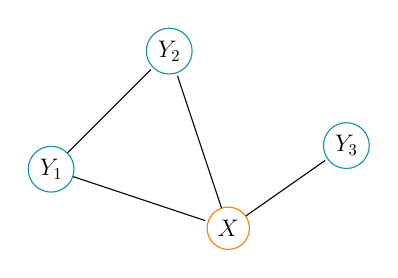
\begin{tikzpicture}
     
      \tikzstyle{every edge}=[-,>=stealth',shorten >=1pt,auto,thin,draw]
		\node[observed] (A1) at (0*\edgeunit, 0*\edgeunit) {$Y_1$};
	\node[bigMissing] (A2) at (1.5*\edgeunit, -0.5*\edgeunit) {
		$X$};
	
		\node[observed] (A3) at (1*\edgeunit, 1*\edgeunit) {$Y_2$};
		\node[observed] (A4) at (2.5*\edgeunit, 0.2*\edgeunit) {$Y_3$};
		\path (A1) edge [] (A2)
        (A1) edge [] (A3)
        (A2) edge [] (A3)
        (A2) edge [] (A4);
\end{tikzpicture}
\end{tabular}\\
 \end{flushright}
 \end{column}
 \begin{column}{0.1\linewidth}
\begin{center}
 $\Longrightarrow$
\end{center}
\end{column}
 \begin{column}{0.4\linewidth}
 \begin{flushleft}
\vspace{0.8cm}
\begin{tabular}{c}
  {Marginal graph}:\\\\
 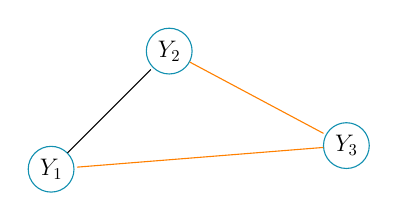
\begin{tikzpicture}
      \tikzstyle{every edge}=[-,>=stealth',shorten >=1pt,auto,thin,draw]
		\node[observed] (A1) at (0*\edgeunit, 0*\edgeunit) {$Y_1$};
		%\node[observed] (A2) at (1.5*\edgeunit, -0.5*\edgeunit) {$A_2$};
		\node[observed] (A3) at (1*\edgeunit, 1*\edgeunit) {$Y_2$};
		\node[observed] (A4) at (2.5*\edgeunit, 0.2*\edgeunit) {$Y_3$};
		\path  (A1) edge [] (A3)
        (A3) edge [orange] (A4)
        (A4) edge [orange] (A1);
\end{tikzpicture}
\end{tabular}\\
\end{flushleft}
Spurious edges leading to wrong interpretation\\
 \end{column}
\end{columns}
\bigskip

$X$ is a \emphase{covariate} or a \emphase{species} unaccounted for in the model.
\end{frame}
% \begin{frame}{Decomposable graphs}
% \begin{itemize}
% \item separation
% \item recursive definition
% \item example
% \item chordal graphs
% \end{itemize}
% \end{frame}
 %=======================================

% \begin{frame}{Hammerslay-Clifford's Theorem}
% $\mathcal{C}$ denotes the set of cliques of $\G$. For any  $C \subset V$, $\psi_C$ is a positive function of $X_C$ only.
% \begin{block}{Theorem - Hammerslay-Clifford}
% For any graph $\G$ and probability distribution $P$ with \emphase{strictly positive} and \emphase{continuous} density $f$ with respect to a product measure, it holds that:
%$$ P\text{ is global Markov relative to }\G \iff f(X) = \prod_{c\in \mathcal{C} }\psi_c(X)$$
% \end{block}
% \end{frame}
 %=======================================

% \begin{frame}{Caution \emphase{/!$\backslash$}}
%The global Markov property is an implication:\\
%\begin{itemize}
% \item A graphical model might not represent all conditional independence relationships.
% \item All probability measures are global Markov relative to the complete graph.
% \end{itemize}
% \bigskip
% If equivalence, $P$ is \emphase{faithful Markov}: an edge in $\G$ means a conditional dependence in the data.
% \end{frame}
 %=======================================

 \begin{frame}{Gaussian Graphical Models (GGM)}
  Let $\Ybf\sim \mathcal{N}(\mu, \Sigmab)$ with precision matrix $\Omegab=\Sigmab^{-1}=(\omega_{jk})_{jk}$:
 $$f(\Ybf) \propto \prod_{j,k,, {\omega_{jk}\neq 0}} \exp(-Y_{k}\omega_{jk}Y_{j}/2).$$
\emphase{Faithful} Markov property:
\vspace{0.3cm}
\begin{columns}
\begin{column}{0.4\linewidth}
  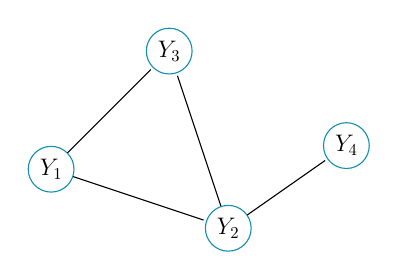
\begin{tikzpicture}
      \tikzstyle{every edge}=[-,>=stealth',shorten >=1pt,auto,thin,draw]
		\node[observed] (A1) at (0*\edgeunit, 0*\edgeunit) {$Y_1$};
	\node[observed] (A2) at (1.5*\edgeunit, -0.5*\edgeunit) {$Y_2$};
		\node[observed] (A3) at (1*\edgeunit, 1*\edgeunit) {$Y_3$};
		\node[observed] (A4) at (2.5*\edgeunit, 0.2*\edgeunit) {$Y_4$};
		\path (A1) edge [] (A2)
        (A1) edge [] (A3)
        (A2) edge [] (A3)
        (A2) edge [] (A4);
       % (A1) edge[Complement,dashed] (A4)
        %(A3) edge[Complement,dashed] (A4);
\end{tikzpicture}
\end{column}
\begin{column}{0.1\linewidth}
\emphase{$\iff$ }
\end{column}
\begin{column}{0.4\linewidth}
$\Omegab=\left(\begin{array}{llll}
*&*&*&\emphase{0}\\
*&*&*&*\\
*&*&*&\emphase{0}\\
\emphase{0}&*&\emphase{0}&*
\end{array}\right) $
\end{column}
\end{columns}

 \end{frame}
 
%=======================================

% \begin{frame}{Classical network inference}
% In the context of Gaussian data $X\sim \Ncal(\mu, \Omegab^{-1})$:
%  $$L(X;\Omegab) = \log |\Omegab| +tr (X^\intercal X \Omegab)+cst .$$
%\begin{block}{Graphical Lasso}
% The glasso estimates the precision matrix as the matrix maximizing the $\ell_1$ penalized log-likelihood:
% $$\widehat{\Omegab}_\lambda=\argmax_{\Omegab\geq 0} \big\{L(\Omegab) - \lambda ||\Omegab||_1\big\}, \qquad ||\Omegab||_1 = \sum_{k\neq l} |\omega_{kl}|.$$
%\end{block}
%\begin{itemize}
%\item Sparse approach: exact zeros in $\widehat{\Omegab}_\lambda$.
%\item Procedures to choose  $\lambda^*$
%\end{itemize}
% \end{frame}
 %=======================================

 \subsection{Graph exploration with trees}
 \begin{frame}{Exploring the graph space}
Aim: infer $\Gb$.\\
Very large space to explore: \emphase{$\text{\#} \mathcal{G}_p = 2^{\frac{p(p-1)}{2}}$}\\
\bigskip
	
	\bleu{Spanning trees} are sparse and simple structures:\\
%	 $$
%  \left. \begin{tabular}{l}
%          $T$ is connected \\
%          $T$ has no cycle
%         \end{tabular} \right\}
%  \text{ $T$ has $(p-1)$ edges.}
%  $$

  \begin{columns}
  \begin{column}{6cm}
	\begin{figure}[htp]
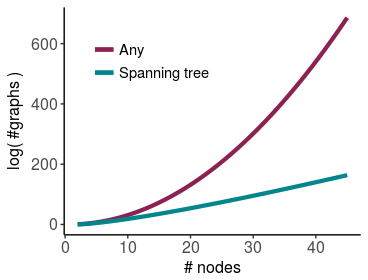
\includegraphics[width=5cm]{images/compar_typegraphs.png}
	\end{figure}
	\end{column}
	 \begin{column}{6cm}
	 \begin{columns}
	 \begin{column}{0.5\linewidth}
	 \begin{itemize}
	 \item no loops
	 \item $(p-1)$ edges
	 \end{itemize}
	 \end{column}
	 \begin{column}{0.5\linewidth}
	 	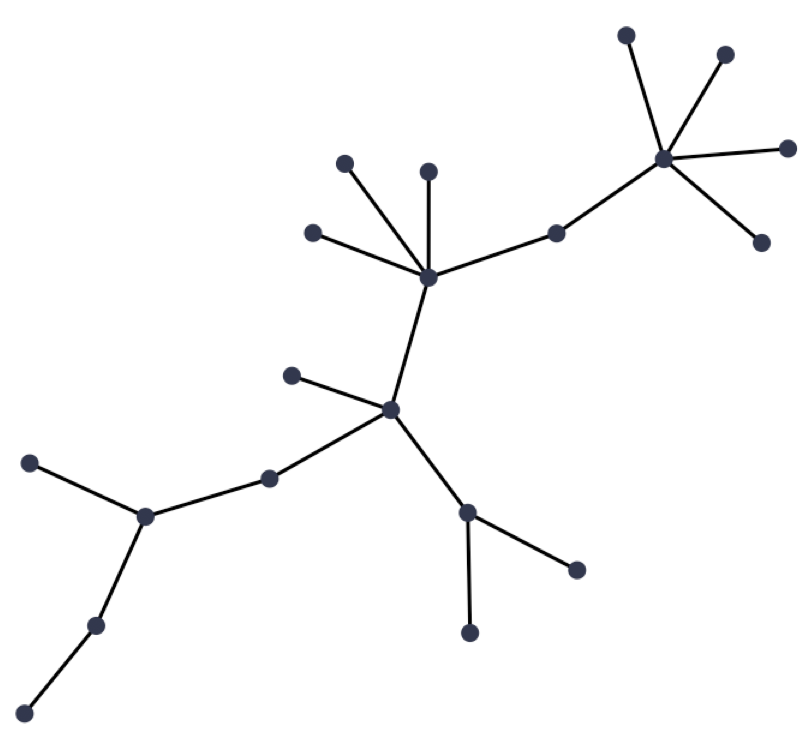
\includegraphics[width=3cm]{images/tree.png} 
	 \end{column}
	  \end{columns}
 \vspace{0.3cm}
 
Much \bleu{ smaller space} to explore:\\  \emphase{$$\text{\#} \mathcal{T}_p = p^{(p-2)}$$}\\ 
 %Idea:  explore a constrained version of the graph space. \bigskip
\end{column}
\end{columns}
 \end{frame}
   %=======================================

 \begin{frame}{Summing over spanning trees}
Let $\Wb=(w_{jk})_{jk}$ be a matrix with null diagonal and positive entries, and $\Qb$ its Laplacian:
$$[\Qb]_{jk}=\left\{ 
					\begin{array}{ll}
						\sum_k w_{jk}& \text{ if } j=k\\
						-w_{jk} & \text{otherwise }
					\end{array}
				\right.$$
\begin{block}{Matrix-tree Theorem \citep{matrixtree} }
All minors of $\Qb$ are equal, and for any $1\leq u, v, \leq p$:
$$ |\Qb^{uv}|= \sum_{T\in\mathcal{T}}\prod_{jk \in T} w_{jk} $$
\end{block} 
Allows to \emphase{sum over $p^{(p-2)}$ trees in $\mathcal{O}(p^3)$} operations.
 \end{frame}
  %=======================================
 
 \begin{frame}{Exploring $\mathcal{T}$ with tree averaging }

\begin{columns}

\begin{column}{0.45\linewidth}
%\only<1>{\begin{tabular}{c}
%	\begin{tikzpicture}
% \tikzstyle{every edge}=[-,>=stealth',shorten >=1pt,auto,thin,draw]
%		\node[basic] (Z1) at (0*\edgeunit, 0*\edgeunit) {};
%		\node[basic] (Z2) at (1*\edgeunit, 0*\edgeunit) {};
%		\node[basic] (Z3) at (1*\edgeunit, 1*\edgeunit) {};
%		\node[basic] (Z4) at (0*\edgeunit, 1*\edgeunit) {};
%		\path (Z1) edge [] (Z2)
%        (Z1) edge [] (Z3)
%        (Z2) edge [] (Z4);
%	\end{tikzpicture}\\
%	\small{$p(T=t_1) = 0.12$}
%\end{tabular}}
%	   
%\only<2>{\begin{tabular}{c}
%\begin{tikzpicture}
%\tikzstyle{every basic}=[draw=none,text=black,scale=0.5,
%      transform shape,circular drop shadow] 
%		\node[basic] (Z1) at (0*\edgeunit, 0*\edgeunit) {};
%		\node[basic] (Z2) at (1*\edgeunit, 0*\edgeunit) {};
%		\node[basic] (Z3) at (1*\edgeunit, 1*\edgeunit) {};
%		\node[basic] (Z4) at (0*\edgeunit, 1*\edgeunit) {};
%		\path (Z1) edge [] (Z2)
%        (Z1) edge [] (Z3)
%        (Z1) edge [] (Z4);
%		\end{tikzpicture} \\
%		\small{$p(T=t_2) = 0.51$}
%	   \end{tabular}}
%	   
%\only<3>{\begin{tabular}{c}
%\begin{tikzpicture}
%\tikzstyle{every basic}=[draw=none,text=black,scale=0.5,
%      transform shape,circular drop shadow] 
%		\node[basic] (Z1) at (0*\edgeunit, 0*\edgeunit) {};
%		\node[basic] (Z2) at (1*\edgeunit, 0*\edgeunit) {};
%		\node[basic] (Z3) at (1*\edgeunit, 1*\edgeunit) {};
%		\node[basic] (Z4) at (0*\edgeunit, 1*\edgeunit) {};
%		\path (Z1) edge [] (Z2)
%        (Z2) edge [] (Z3)
%        (Z2) edge [] (Z4); 
%\end{tikzpicture}\\
%		\small{$p(T=t_3) = 0.02$}
%		\end{tabular}}
%	   
%\only<4>{\begin{tabular}{c}
%\begin{tikzpicture}
%\tikzstyle{every basic}=[draw=none,text=black,scale=0.5,
%      transform shape,circular drop shadow] 
%		\node[basic] (Z1) at (0*\edgeunit, 0*\edgeunit) {};
%		\node[basic] (Z2) at (1*\edgeunit, 0*\edgeunit) {};
%		\node[basic] (Z3) at (1*\edgeunit, 1*\edgeunit) {};
%		\node[basic] (Z4) at (0*\edgeunit, 1*\edgeunit) {}; 
%		\path (Z1) edge [] (Z2)
%        (Z3) edge [] (Z4)
%        (Z2) edge [] (Z4);
%\end{tikzpicture} \\
%		\small{$p(T=t_4) = 0.3$}
%\end{tabular}}

%\only<5-6>{	 
\begin{tabular}{c}

\begin{tabular}{m{1cm} m{2cm}}
	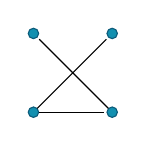
\begin{tikzpicture}
 \tikzstyle{every edge}=[-,>=stealth',shorten >=1pt,auto,thin,draw]
		\node[basic] (Z1) at (0*\smalledgeunit, 0*\smalledgeunit) {};
		\node[basic] (Z2) at (1*\smalledgeunit, 0*\smalledgeunit) {};
		\node[basic] (Z3) at (1*\smalledgeunit, 1*\smalledgeunit) {};
		\node[basic] (Z4) at (0*\smalledgeunit, 1*\smalledgeunit) {};
		\path (Z1) edge [] (Z2)
        (Z1) edge [] (Z3)
        (Z2) edge [] (Z4);
	\end{tikzpicture} &
	\small{$p(t_1) = 0.12$}
\end{tabular}\\

\begin{tabular}{m{1cm} m{2cm}}
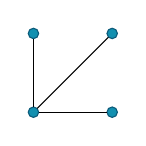
\begin{tikzpicture}
\tikzstyle{every basic}=[draw=none,text=black,scale=0.5,
      transform shape,circular drop shadow] 
		\node[basic] (Z1) at (0*\smalledgeunit, 0*\smalledgeunit) {};
		\node[basic] (Z2) at (1*\smalledgeunit, 0*\smalledgeunit) {};
		\node[basic] (Z3) at (1*\smalledgeunit, 1*\smalledgeunit) {};
		\node[basic] (Z4) at (0*\smalledgeunit, 1*\smalledgeunit) {};
		\path (Z1) edge [] (Z2)
        (Z1) edge [] (Z3)
        (Z1) edge [] (Z4);
		\end{tikzpicture} &
		\small{$p(t_2) = 0.51$}
	   \end{tabular}\\
	   
	   \begin{tabular}{m{1cm} m{2cm}}
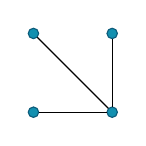
\begin{tikzpicture}
\tikzstyle{every basic}=[draw=none,text=black,scale=0.5,
      transform shape,circular drop shadow] 
		\node[basic] (Z1) at (0*\smalledgeunit, 0*\smalledgeunit) {};
		\node[basic] (Z2) at (1*\smalledgeunit, 0*\smalledgeunit) {};
		\node[basic] (Z3) at (1*\smalledgeunit, 1*\smalledgeunit) {};
		\node[basic] (Z4) at (0*\smalledgeunit, 1*\smalledgeunit) {};
		\path (Z1) edge [] (Z2)
        (Z2) edge [] (Z3)
        (Z2) edge [] (Z4); 
\end{tikzpicture}&
		\small{$p(t_3) = 0.02$}
		\end{tabular}\\

\begin{tabular}{m{1cm} m{2cm}}
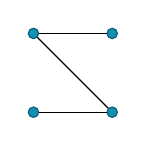
\begin{tikzpicture}
\tikzstyle{every basic}=[draw=none,text=black,scale=0.5,
      transform shape,circular drop shadow] 
		\node[basic] (Z1) at (0*\smalledgeunit, 0*\smalledgeunit) {};
		\node[basic] (Z2) at (1*\smalledgeunit, 0*\smalledgeunit) {};
		\node[basic] (Z3) at (1*\smalledgeunit, 1*\smalledgeunit) {};
		\node[basic] (Z4) at (0*\smalledgeunit, 1*\smalledgeunit) {}; 
		\path (Z1) edge [] (Z2)
        (Z3) edge [] (Z4)
        (Z2) edge [] (Z4);
\end{tikzpicture} &
		\small{$p(t_4) = 0.3$}
\end{tabular}\\

\Large{\textbf{.}}\\
\Large{\textbf{.}}\\
\Large{\textbf{.}}

\end{tabular}%}
\end{column}
%\pause
\begin{column}{0.45\linewidth}
\begin{center}
%\only<6>{
Network inference \\= edge probabilities:\\
		\vspace{0.5cm}
		
\begin{tabular}{c}
		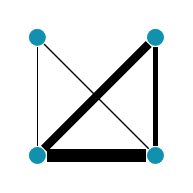
\begin{tikzpicture}
			\node[large] (Z1) at (0*\edgeunit, 0*\edgeunit) { };
		\node[large] (Z2) at (1*\edgeunit, 0*\edgeunit) { };
		\node[large] (Z3) at (1*\edgeunit, 1*\edgeunit) { };
		\node[large] (Z4) at (0*\edgeunit, 1*\edgeunit) { };
		\draw [line width=5pt] (Z1) -- (Z2); 
		\draw [line width=3pt] (Z1) -- (Z3); 
		\draw [line width=.5pt] (Z1) -- (Z4); 
		\draw [line width=2pt] (Z2) -- (Z3); 
		\draw [line width=.5pt] (Z2) -- (Z4); 
 %		\draw [line width=.5pt] (Z3) -- (Z4); 
		\end{tikzpicture}   \end{tabular}\\
		
		\vspace{0.5cm}
		
		$\displaystyle{\mathds{P}\{k\ell\in T \}= \emphase{\sum_{\substack{T \in \mathcal{T}\\ k\ell\in T}}} p(T)}$
		\vspace{0.3cm}
		
 $p(T)\propto \prod_{kl\in T} w_{kl}$
	%   }
	   \end{center}
\end{column}

\end{columns}
 \end{frame}

  %=======================================

% \begin{frame}{Handy law}
% \begin{itemize}
% \item Law decomposable on the edges
% \end{itemize}
% \end{frame}

  %=======================================

% \begin{frame}{Network inference from Gaussian data with trees}
% \begin{itemize}
% \item def gaussian tree mixture
% \item what it means : the underlying graphical model is assumed to be a \emphase{tree} which is \emphase{random}.
% \end{itemize}
% \end{frame}
  %=======================================

% \begin{frame}{Generalized Linear Mixed Models (GLMM)}
% \begin{itemize}
% \item definition
% \item easy handling of covariates and offsets
% \item possible with less latent variables : latent variable model
% \end{itemize}
% \end{frame}
  %=======================================

 \subsection{Poisson log-Normal model}
 \begin{frame}{Getting back to Gaussian data}
 \begin{center}
\begin{tikzpicture}
      \tikzstyle{every edge}=[-,>=stealth',shorten >=1pt,auto,thin,draw]
		\node (A1) at (0*\edgeunit, 0*\edgeunit) {
		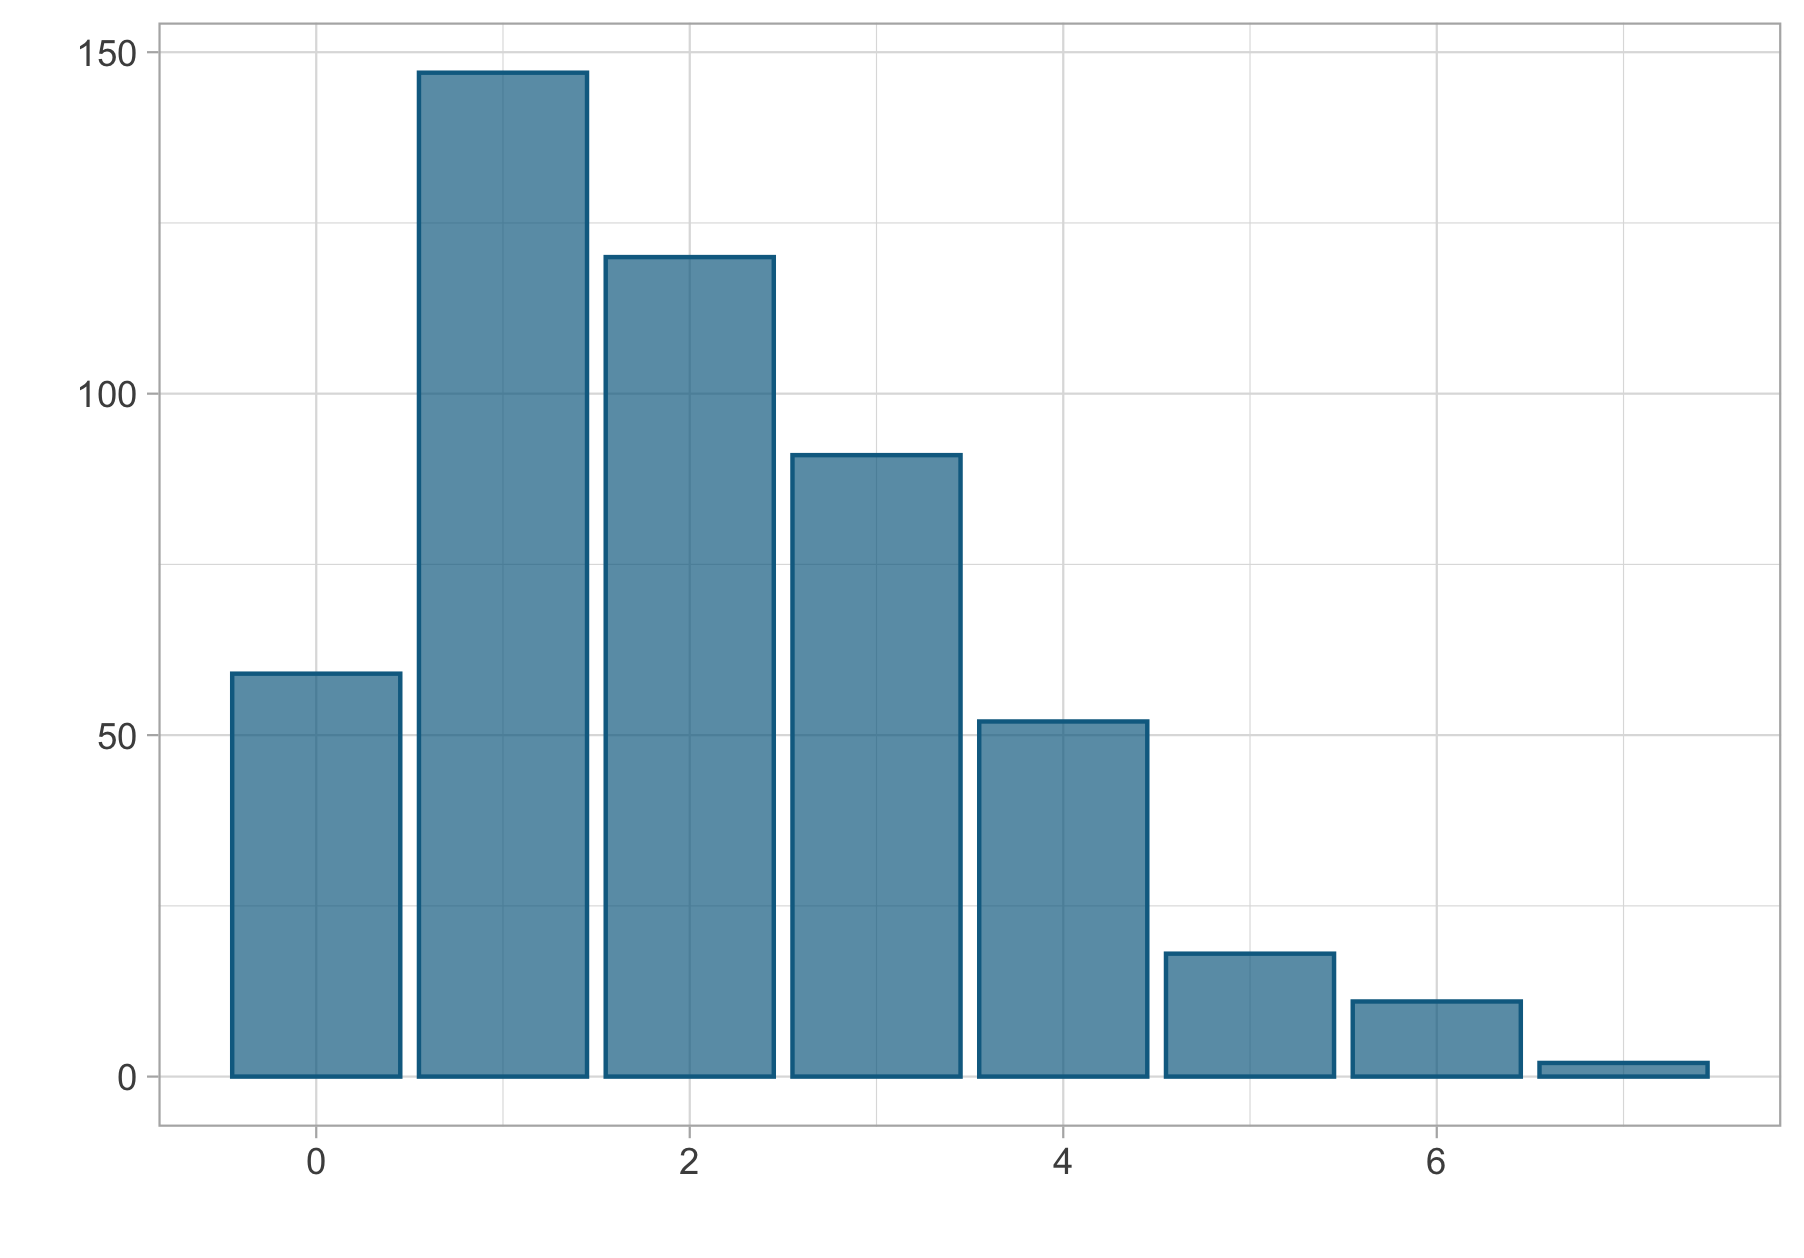
\includegraphics[width=3cm]{images/discret.png}};
		\node (A2) at (5*\edgeunit, 0*\edgeunit) {
		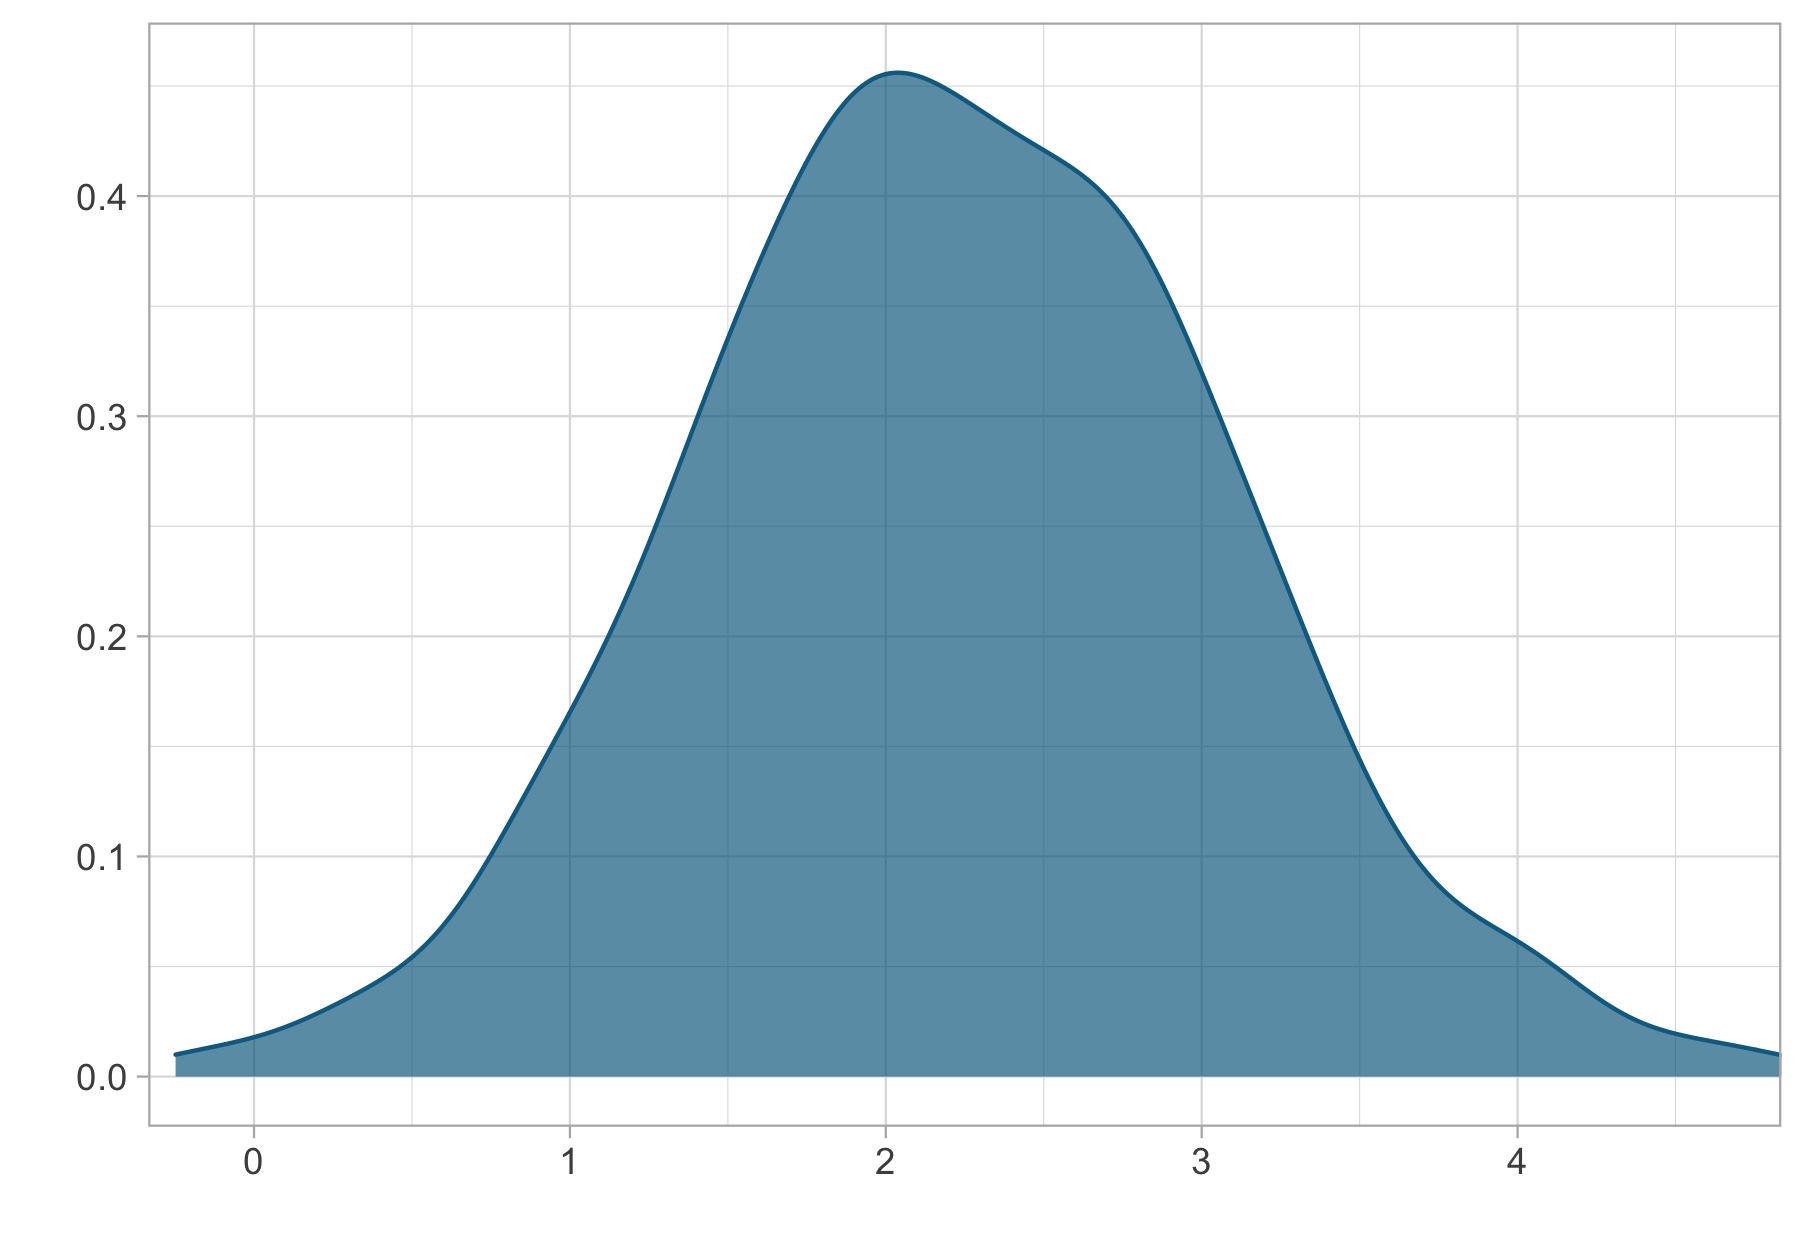
\includegraphics[width=3cm]{images/continu.png}};
	 \node (A3) at (2.5*\edgeunit, 1.25*\edgeunit) {\text{Transformations}};
	  \node (A4) at (2.5*\edgeunit, 0.15*\edgeunit) {\text{Copulas}};
	   
		\path (A1) edge [->, bend left] (A2) 
		(A1) edge [->] (A2);
	
		\node (A5) at (2.5*\edgeunit, -1.25*\edgeunit) {\emphase{\text{Latent variables}}};
		\path (A1) edge [->, bend right] (A2) ;
	% \pause 
		\node (A6) at (2.5*\edgeunit, -2.5*\edgeunit) {\text{Modeling counts with Gaussian latent parameters}};
		\path (A5) edge [->] (A6) ;
\end{tikzpicture}
 \end{center}
 \end{frame}

  %=======================================

 \begin{frame}{Poisson log-normal model}
 P$\ell$N model \citep{AiH89} for sample $i$ and species $j$:
 \begin{align*}
   \Zbf_i  &\sim \Ncal (0, \Sigmab)\\\\
 Y_{ij}\mid \Zbf_i&\sim \Pcal (\exp (\underbrace{o_{ij}+\xb_i^\intercal \thetab_j}_{\text{fixed}}+ Z_{ij})).
  \end{align*}
 \begin{itemize}
 \item Latent variables are iid, observed data are independent conditionally on the $\Zbf_i$.
 \item A generalized multivariate linear mixed model : fixed abiotic and random biotic effects.
 \item Variational estimation algorithm (PLNmodels, \citet{CMR18}) 
 \end{itemize}
 \end{frame}
 

 %%%%%%%%%%%%%%%%%%%%%%%%%%%%%%%%%%
%%%%%%%%%%%%%%%%%%%%%%%%%%%%%%%%%%
 
\section{Network inference from counts}
\begin{frame}{}
\begin{center}
\Huge{\bleu{Network inference from counts}}
\end{center}
\begin{center}
\begin{description}
\item[i] Model
\item[ii]  Inference
\item[iii] Illustration
\end{description}
\end{center}
\end{frame}
 %=======================================
\subsection{Model}
 \begin{frame}{General model}
 \begin{columns}
 
 \begin{column}{0.45\linewidth}
  \begin{itemize}
  \item Assume a random tree dependency structure $T$\vspace{0.3cm}
  
 \item Dependence structure in  Gaussian layer $\Zbf$\vspace{0.3cm}
 
 \item Distribution for counts $\Ybf$ accounting for covariates/offsets
 \end{itemize}
 \end{column}

 \begin{column}{0.1\linewidth}
  \begin{center}
	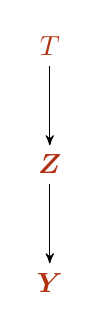
\begin{tikzpicture}	
      \tikzstyle{every edge}=[-,>=stealth',auto,thin,draw]
		\node (A1) at (0*\length, 2*\length) {\emphase{$T$}};
		\node (A2) at (0*\length, 1*\length) {\emphase{$\Zbf$}};
		\node (A3) at (0*\length, 0*\length) {\emphase{$\Ybf$}};
		\draw (A1) edge [->](A2);
        \draw (A2) edge [->] (A3);
	\end{tikzpicture} 
   \end{center}
%   \vspace{0.5cm}
  \end{column}
  
 \begin{column}{0.45\linewidth}
 \begin{itemize}
  \item Matrix Tree Theorem \vspace{0.6cm}
  \item Gaussian Graphical Model \vspace{0.6cm}
  \item Poisson log-normal model\vspace{0.6cm}
  \end{itemize}
 \end{column}
   \end{columns}

 \end{frame}
  %=======================================

 \begin{frame}{$P\ell N$ model with tree-shaped Gaussian parameters}
  \only<1-2>{
\begin{equation*}
  \begin{array}{l}
 \begin{array}{l}
 T\sim \prod_{kl\in T} \beta_{kl} / B,  \\\\
\pause \Zbf_i\mid T  \sim \Ncal (0, \Omegab_T),  
 \end{array} \\\\
\pause Y_{ij}\mid \Zbf_i\sim \Pcal (\exp (o_{ij}+\xb_i^\intercal \thetab_j + Z_{ij})).  
 \end{array}  
 \end{equation*}}
 \only<3>{
 \begin{equation*}
    \left\{\begin{array}{l}
 T\sim \prod_{kl\in T} \beta_{kl} / B, \\\\
 \Zbf_i\mid T  \sim \Ncal (0, \Omegab_T)\\\\
 Y_{ij}\mid \Zbf_i\sim \Pcal (\exp (o_{ij}+\xb_i^\intercal \thetab_j + Z_{ij})).
 \end{array}   \right.
 \end{equation*}}
 \bigskip
 
 Gaussian mixture with $p^{p-2}$ components:
 $$p(\Zbf) = \sum_{T\in \mathcal{T}} p(T) \Ncal(\Zbf\mid T ; 0, \Omegab_T).$$
Decomposition of the likelihood:
 $$p(\Ybf, \Zbf,T)=p_{\emphase{\betab}}(T)\;p_{\emphase{\Omega_T}}(\Zbf\mid T)\;p_{\emphase{\thetab}}(\Ybf\mid \Zbf).$$
 \end{frame}
 
 \subsection{Inference}
  %=======================================
  \begin{frame}{Two-step procedure}
    \begin{block}{EM algorithm \citep{DLR77}}
 Maximizes the likelihood in presence of latent variables: \vspace{0.2cm}
 
  \begin{description}
  \item[E step:] \vspace{-0.2cm} Compute $\Esp[\log p_{\Theta^t}(\Ybf,\Zbf,T)\mid\Ybf]$
  \item[M step:] $\Theta^{t+1}=\argmax_{\Theta}\big\{\Esp[\log p_{\Theta^t}(\Ybf, \Zbf,T)\mid\Ybf]\big\}$
  \end{description}
    \end{block}
    \pause
   \begin{enumerate}
   \item \texttt{PLNmodels} \citep{CMR18} gives $\widehat{\thetab}$ and approximates of $\Zbf \mid \Ybf$ sufficient statistics.
   \item EM algorithm to get  $\widehat{\betab}$.
   \end{enumerate}
   \bigskip
   
 
    Actually: $\tilde{\Esp}[\log p_\beta (\Ybf,\Zbf, T)\mid \Zbf]=\tilde{\Esp}[\log p_\beta (\Zbf, T)\mid \Zbf]+cst$.
  \end{frame}
%=======================================
\begin{frame}{Factorization on the edges}
\emphase{Tree structure factorization}:
$$p_{\Omegab_T}(\Zbf\mid T) = \prod_k p(\Zbf_k) \prod_{kl\in T} \frac{p(\Zbf_k,\Zbf_l)}{p(\Zbf_k)\: p(\Zbf_l)}$$
 Only the $1^{rst}$ and $2^{nd}$ order moments of $\Zbf\mid\Ybf$ are required, replaced by their variational approximation from  step 1.
 \begin{block}{Expression of  the surrogate}
 $$\tilde{\Esp}[\log p_\beta (\Zbf, T)\mid \Zbf] = \sum_{j<k} P_{jk} \log \big(\emphase{\beta_{jk}\widehat{\psi}_{jk} }\big)- \log B + cst,$$
 where $\widehat{\psi}_{jk} = (1-\widehat{\rho}_{jk}^2)^{-n/2}$ and $P_{jk}=\mathds{P}\{jk\in T \mid \Zbf\}$.
 \end{block}
 
\end{frame}


  
  %=======================================
  \begin{frame}{Proposed EM algorithm}
The $M$ matrix is built from the inverse Laplacian minor $(\Qb(\Wb)^{11})^{-1}$ \citep{MeilaJaak}.\vspace{0.5cm}
   
  \begin{description}
  \item[E step:]$p(T\mid\Zbf)$ factorizes on the edges. \\
  Using the weight matrix \emphase{$\Wb = \betab \odot \widehat{\psi}$}, all probabilities can be computed at once:
  \begin{center}
  $P_{jk} = w_{jk} M(\Wb)_{jk}$  \citep{kirshner}  
  \end{center}\vspace{0.5cm}
  \item[M step:] Requires the computation of $\partial_{\beta_{jk}} (\sum_{T\in\mathcal{T}}\prod_{jk\in T} \beta_{jk})$.\\
  Closed form is available:
  \begin{center}
  \emphase{  \large{$\beta_{jk}^{t+1} = \dfrac{P_{jk}^t}{M(\betab^t)_{jk}}$}}
  \end{center}
  This fixed-point problem is solved using optimization, with a gradient ascent procedure.
   \end{description}

  \end{frame}
 
   %================================
   \begin{frame}{Numerical stability and the Matrix Tree Theorem}
   \begin{columns}
   \begin{column}{0.6\linewidth}
   \textit{$\sum_{T\in \mathcal{T}}\prod_{jk \in T} \beta_{jk}$ computable for any $p'$:}
  \begin{itemize} 
   \item  Upper and lower bounds for $\betab$, which depend on $p'$ and the machine precision.
   \end{itemize}
   \bigskip
   
\textit{ If $\betabf$ has too many high values, $\Qb(\betabf)^{11}$ can become numerically non positive-definite (conditioning$<1e-16$):}
      \begin{itemize}
   \item  The mean value is controlled with a sum constraint.
   \end{itemize}
 
   \end{column}
   \begin{column}{0.4\linewidth}
   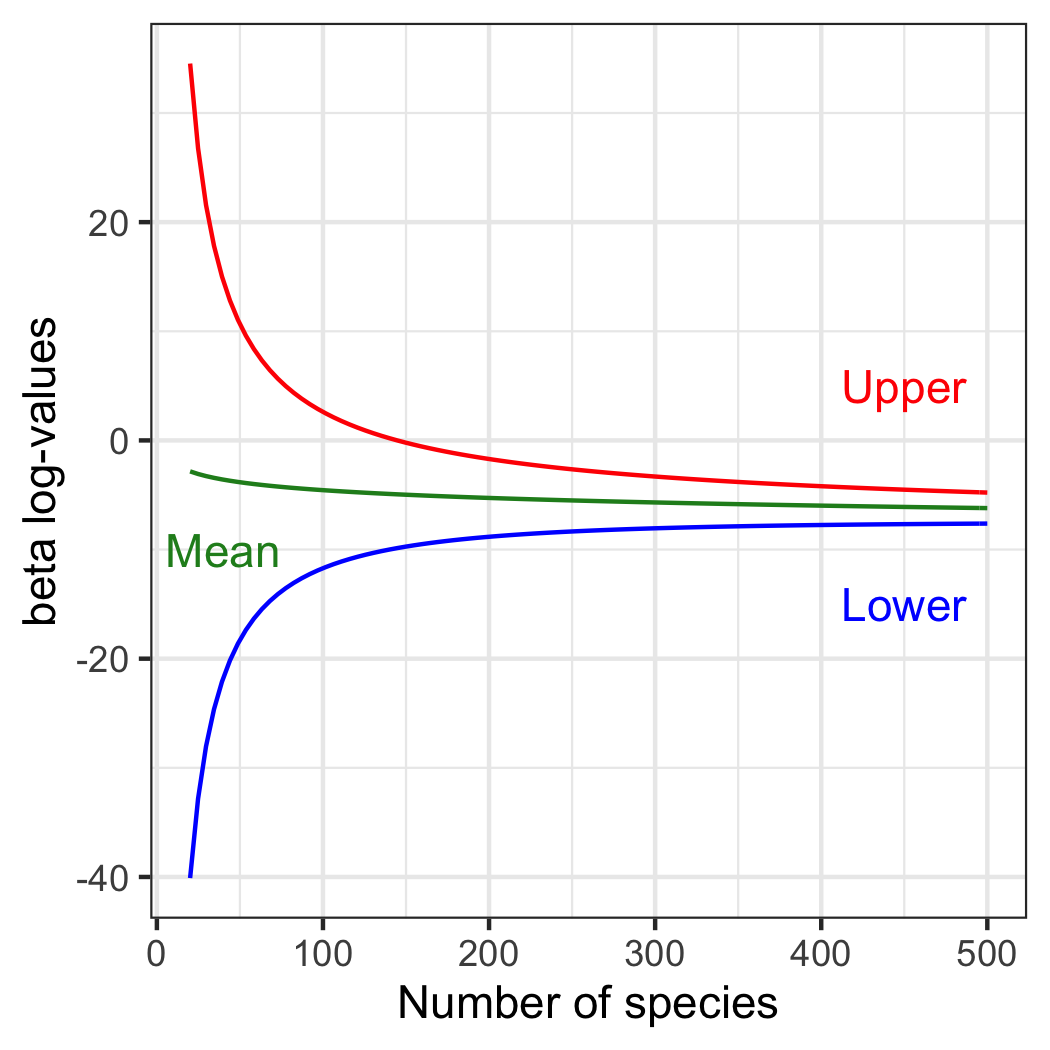
\includegraphics[width=\linewidth]{images/beta_constraints.png}
   \end{column}
   \end{columns}
   \bigskip
   
   These constraints on the optimization improve the algorithm's \emphase{numerical stability} and allows larger networks.
   \end{frame}
   %====================================================================
\begin{frame}{Edge selection frequencies}\small
\begin{enumerate}
\item Create \emphase{$S$ random sub-samples} using $80\%$ of input abundance data
\item \footnotesize $ 
\begin{tabular}{l|rrrrc}
s & \multicolumn{4}{c}{edges probabilities}&\\\hline
1&2e-04& 0.0024& 0.0414 &0.2507&\\
2&1e-04 &0.0013 &0.0004 &0.0574&\\
3&2e-04 &0.0013 &0.0008 &0.0127&...\\
\vdots&\vdots & \vdots & \vdots & \vdots&  
\end{tabular}$
\item   \small
Apply average probability \emphase{$2/p$ threshold} on all resampled probabilities
% \begin{center}
% 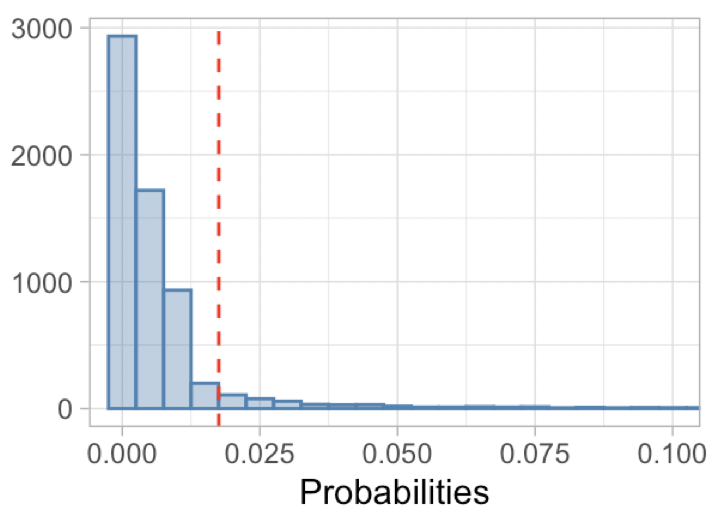
\includegraphics[width=4cm]{images/small_thresh.png}
% \end{center}

\item   $\displaystyle F_{jk} = \sum_{s=1}^S \mathds{1}\{P_{jk}^s\geq 2/p\}/S$\\
Edges selection frequencies:$
\begin{tabular}{rrrrc}
0.000 &0.0381 &0.0190 &0.7048&...
 \end{tabular}$

\end{enumerate}
 \end{frame}
 \begin{frame}{EMtree algorithm}
\begin{description}
\normalsize
\item [Input: ] \hspace{0.35cm}Abundance data, covariates, offsets\vspace{0.2cm}

\item [1rst step: ] \hspace{0.3cm} \emphase{fit PLN model} $\Rightarrow$  $\hat{\theta}$, $\hat{\Sigma}_Z$. \vspace{0.2cm}
\item [2nd step: ] \hspace{0.3cm} \emphase{update the $\beta_{jk}$} $\Rightarrow$ conditional probabilities for all edges.\\ \hspace{0.3cm} 
%\pause
\bigskip
\item [Thresholding: ] Select edges with probability above the probability of edges in a tree drawn uniformly (\emphase{$2/p$})\vspace{0.2cm}
\item [Resampling: ] \hspace{0.25cm}Strengthen the results: keep only edges selected in more than \emphase{$80\%$} of $S$ sub-samples (selection threshold).
\end{description} \bigskip

Available for download at \url{https://github.com/Rmomal/EMtree}
\begin{figure}
    \centering
    
\includegraphics[width=0.6cm]{images/github.png}
\end{figure}
\end{frame}
 \subsection{Simulations}
 %=================================
 
 
\begin{frame}{Alternative approaches}
 Three methods  from microbioloby:\\
    \begin{itemize}
        \item \emphase{SpiecEasi} algorithm \citet{kurtz} 
        \item \emphase{gCoda} \citet{gcoda} 
        \item \emphase{MInt} \citet{MInt} (uses PLN model)
    \end{itemize}\bigskip

 Two methods  from ecology:\\
    \begin{itemize}
        \item \emphase{ecoCopula} algorithm \citet{PHW18} 
        \item \emphase{MRFcov} \citet{CWL18} 
    \end{itemize}\bigskip
    
    They all use the Graphical LASSO (glasso, citet{GLasso}).
\end{frame}
 %=================================
\begin{frame}{Edge-scoring with glasso}
L1 penalization of the Gaussian log-likelihood:
 
 \[L(Y,\Omega) = \frac{n}{2}\log |\Omega|-\frac{n}{2} Y^T\Omega Y + cste\]
\[\widehat{\Omega}_{glasso}(\lambda) = \arg\max\left\{ L(Y,\Omega)-\emphase{\lambda} ||\Omega||_1 \right\} \]
The greater the penalty $\emphase{\lambda}$, the more null entries in $\widehat{\Omega}_{glasso}$.\\
\bigskip

The glasso depends on a grid of penalties $\{\lambda_1,...,\lambda_n\}$, each associated with  a different pattern of zeros. We define the score:
\emphase{$$s_{jk}\propto \sum_{\lambda_i} \lambda_i \times \mathds{1}\{\omega_{jk} \neq 0\}$$}
$s_{jk}$ measures the robustness of edge $jk$ in the network.
\end{frame}
 %=================================

\begin{frame}{Simulation design}
\begin{enumerate}
     \item Choose  \emphase{$G$} and randomly define the sign of its entries.
     \item Build \emphase{$\Omega_G=Q(G)+\delta\times I$} and $\Sigma_G=\Omega_G^{-1}$.
     \item Sample count data \emphase{$Y$} from $\mathcal{P\ell N}(X,\Sigma_G)$ with \emphase{covariates}.
     \item Infer the network with all methods.
     \item Compare results with  presence/absence of edges (\emphase{FDR}, \emphase{AUC}).
\end{enumerate}
\bigskip

To account for covariates, SpiecEasi and gCoda are run on residuals of the regression of transformed data.
\end{frame}

%====================================================================
%====================================================================


\begin{frame}{Tested graphs types}
    \begin{tabular}{ccc}
       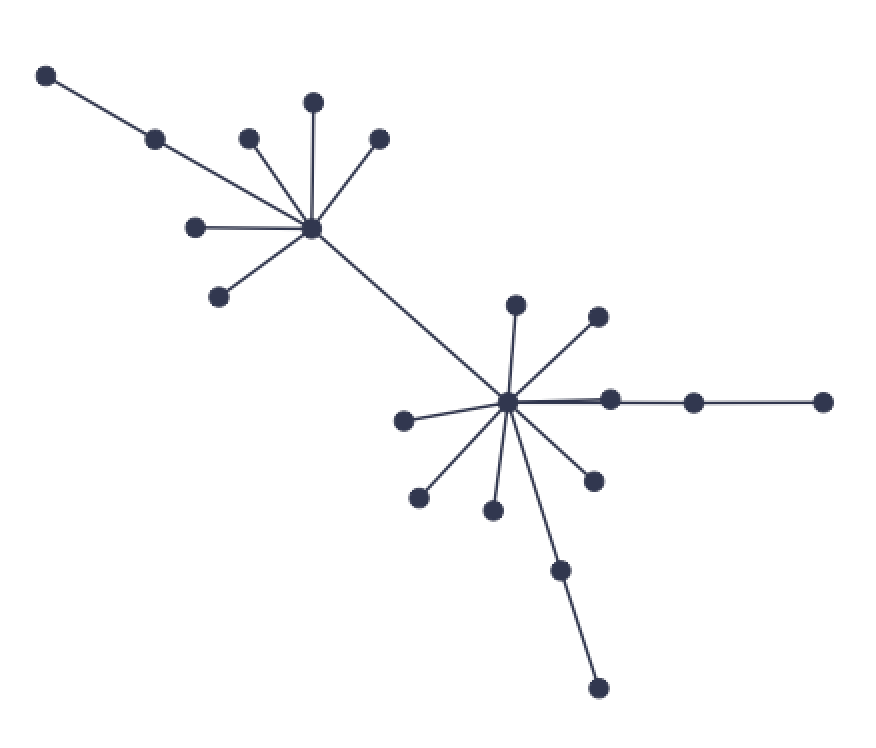
\includegraphics[width=4cm]{images/scale-free.png} &
         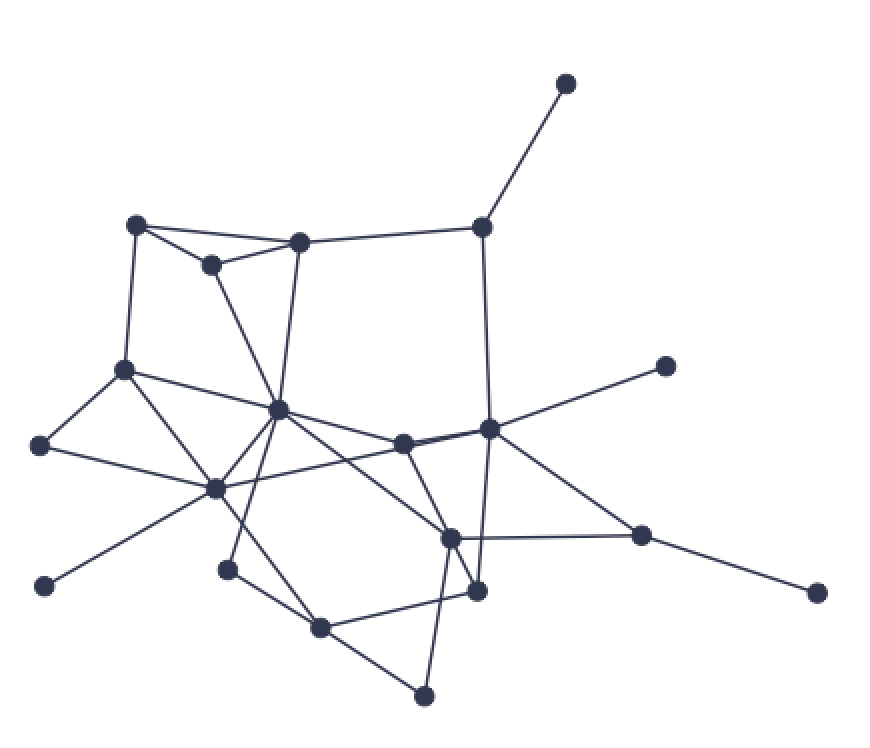
\includegraphics[width=3.5cm]{images/erdos.png}&
            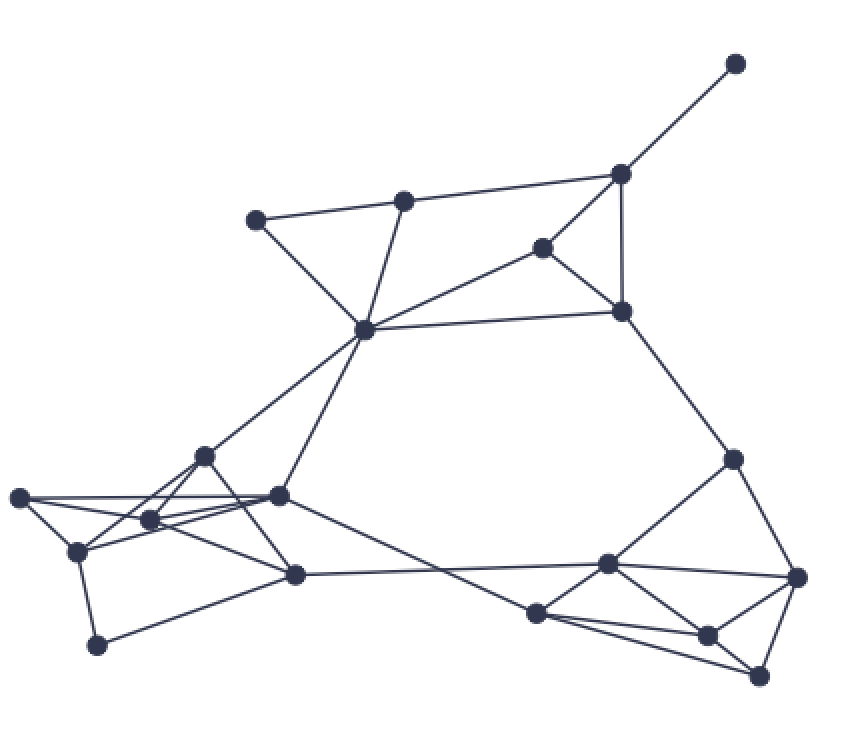
\includegraphics[width=3.5cm]{images/cluster.png}\\
            Scale-free & Erdos & Cluster
    \end{tabular} 
\end{frame}
 %=================================
\begin{frame}{Experiments}
\bleu{Weighted output:}\\
\begin{itemize}
\item Study of EMtree, SpiecEasi and gCoda
\item By default: n=100 and p=20, density=$3/p$
\item AUC for varying values of n,p, and density parameter when available
\end{itemize}
\bigskip

\bleu{Final network:}\\
\begin{itemize}
\item Comparison of all methods optimal networks
\item Two difficulty levels: n=100, p=20 and n=50, p=30
\item FDR and density ratio
\end{itemize}
 \end{frame}
  %=================================
   \begin{frame}{Weighted output comparison}
   \bleu{Area under the (ROC) cruve (AUC)}: measure of the edges ranking quality.
 \begin{center}
  \includegraphics[width=\linewidth]{images/panel_npfav.png}
   \end{center}
  \begin{columns}
  \begin{column}{0.5\linewidth}
  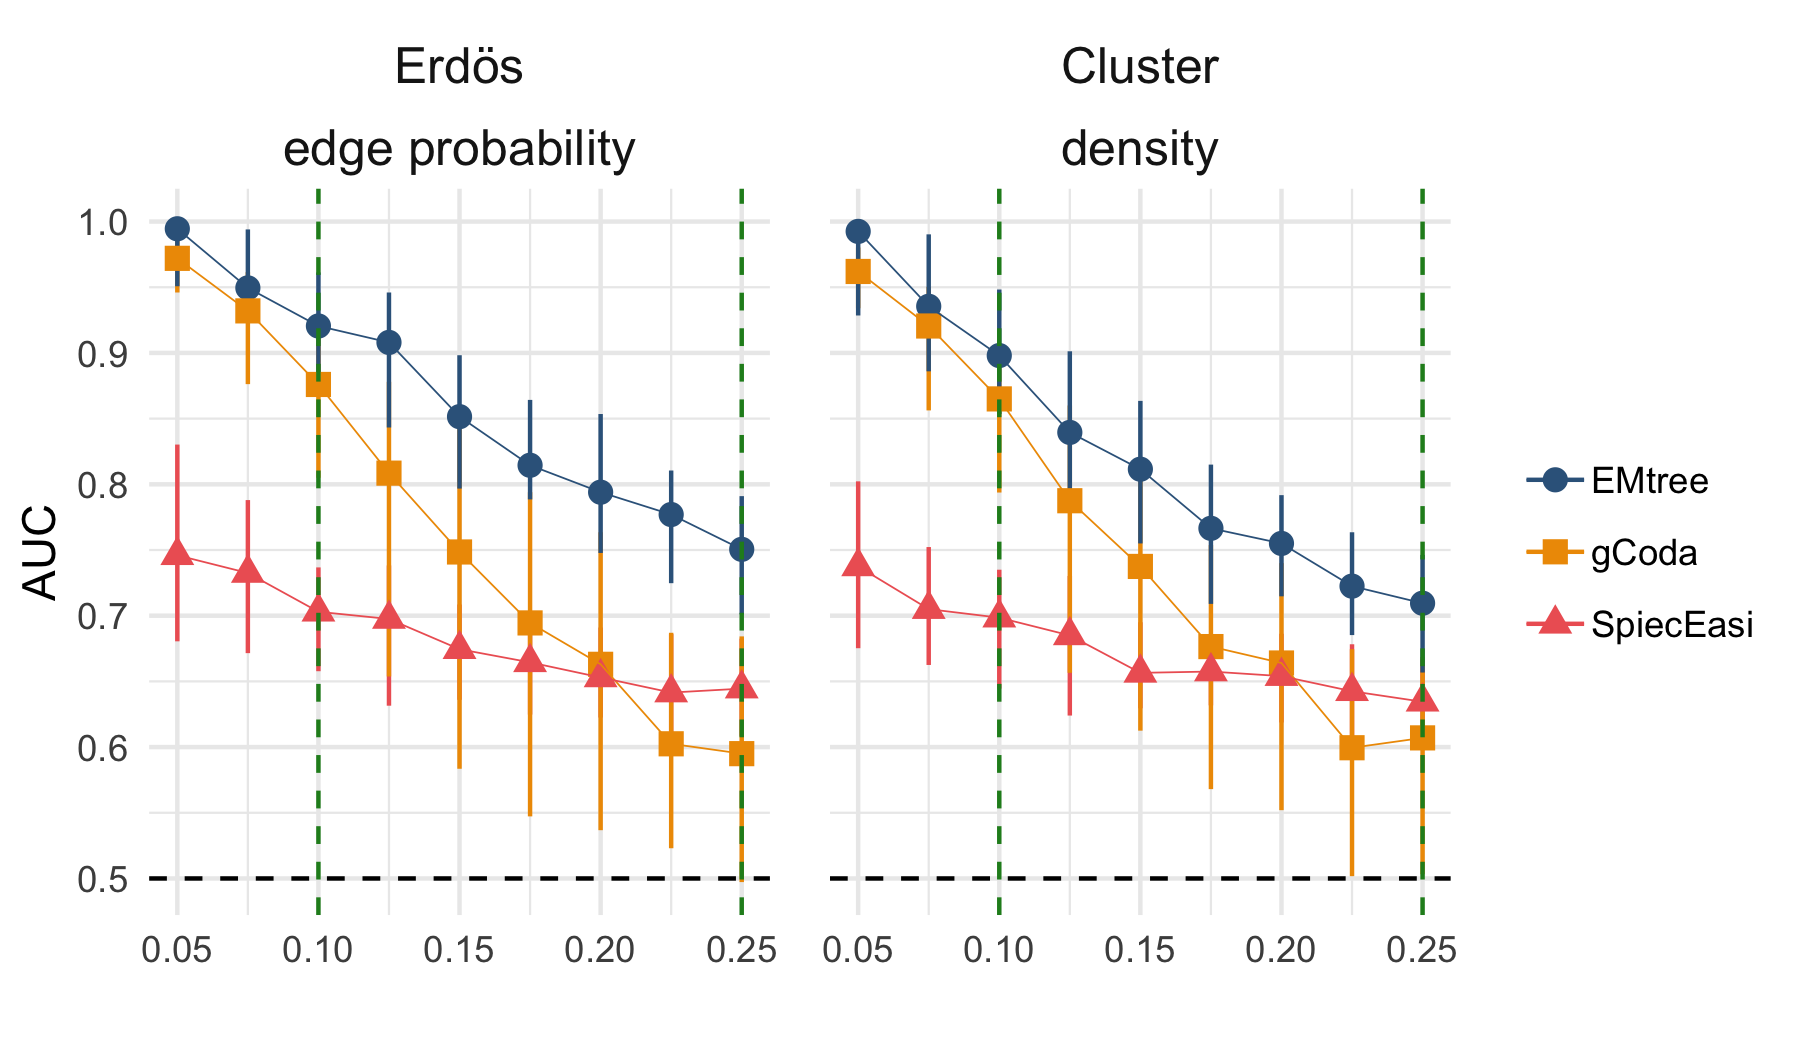
\includegraphics[width=\linewidth]{images/panel_dens_seuils.png} 
  \end{column}
    \begin{column}{0.5\linewidth}
   \begin{itemize}
 \item The more data the better.
 \item The less dense the better.
 \end{itemize}
   \end{column}
   \end{columns}

 \end{frame}
 
 \begin{frame}{Weighted output comparison}
 \begin{center}
  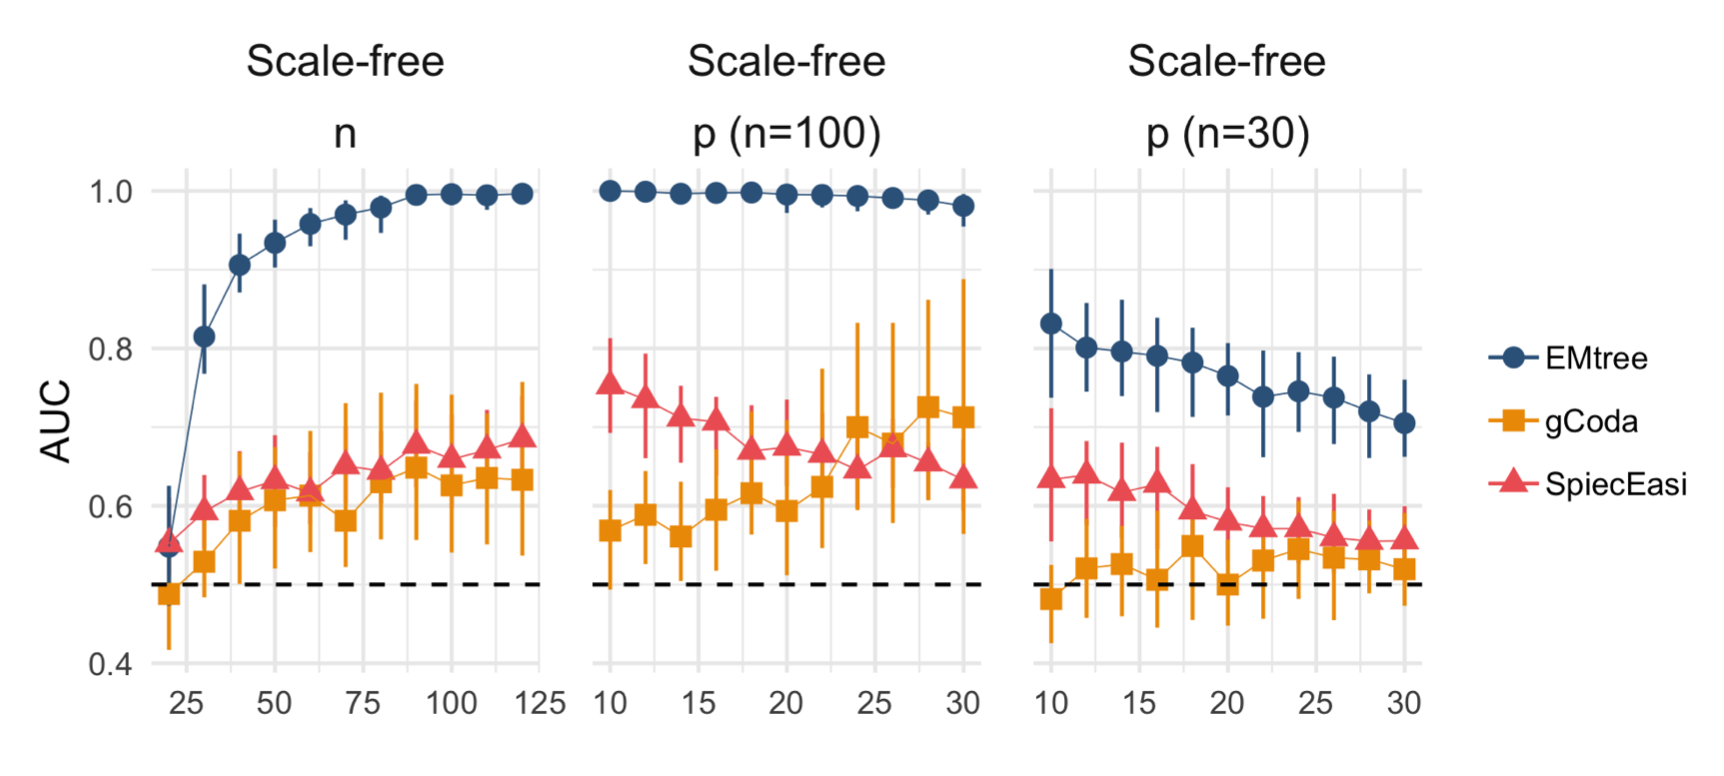
\includegraphics[width=0.7\linewidth]{images/scalef_auc.png}
 \end{center}
 The tree hypothesis of the model does not impair performance for Erdös and Cluster structures, and might improve them for scale-free structures.
 \end{frame}
 
  \begin{frame}{Final networks comparison (Erdös)}
 \small{ \bleu{False Discovery Rate (FDR):} how many false edges among those detected ?\\
  \bleu{Density ratio:} number of detections/number of true edges}\normalsize
 \begin{figure}
 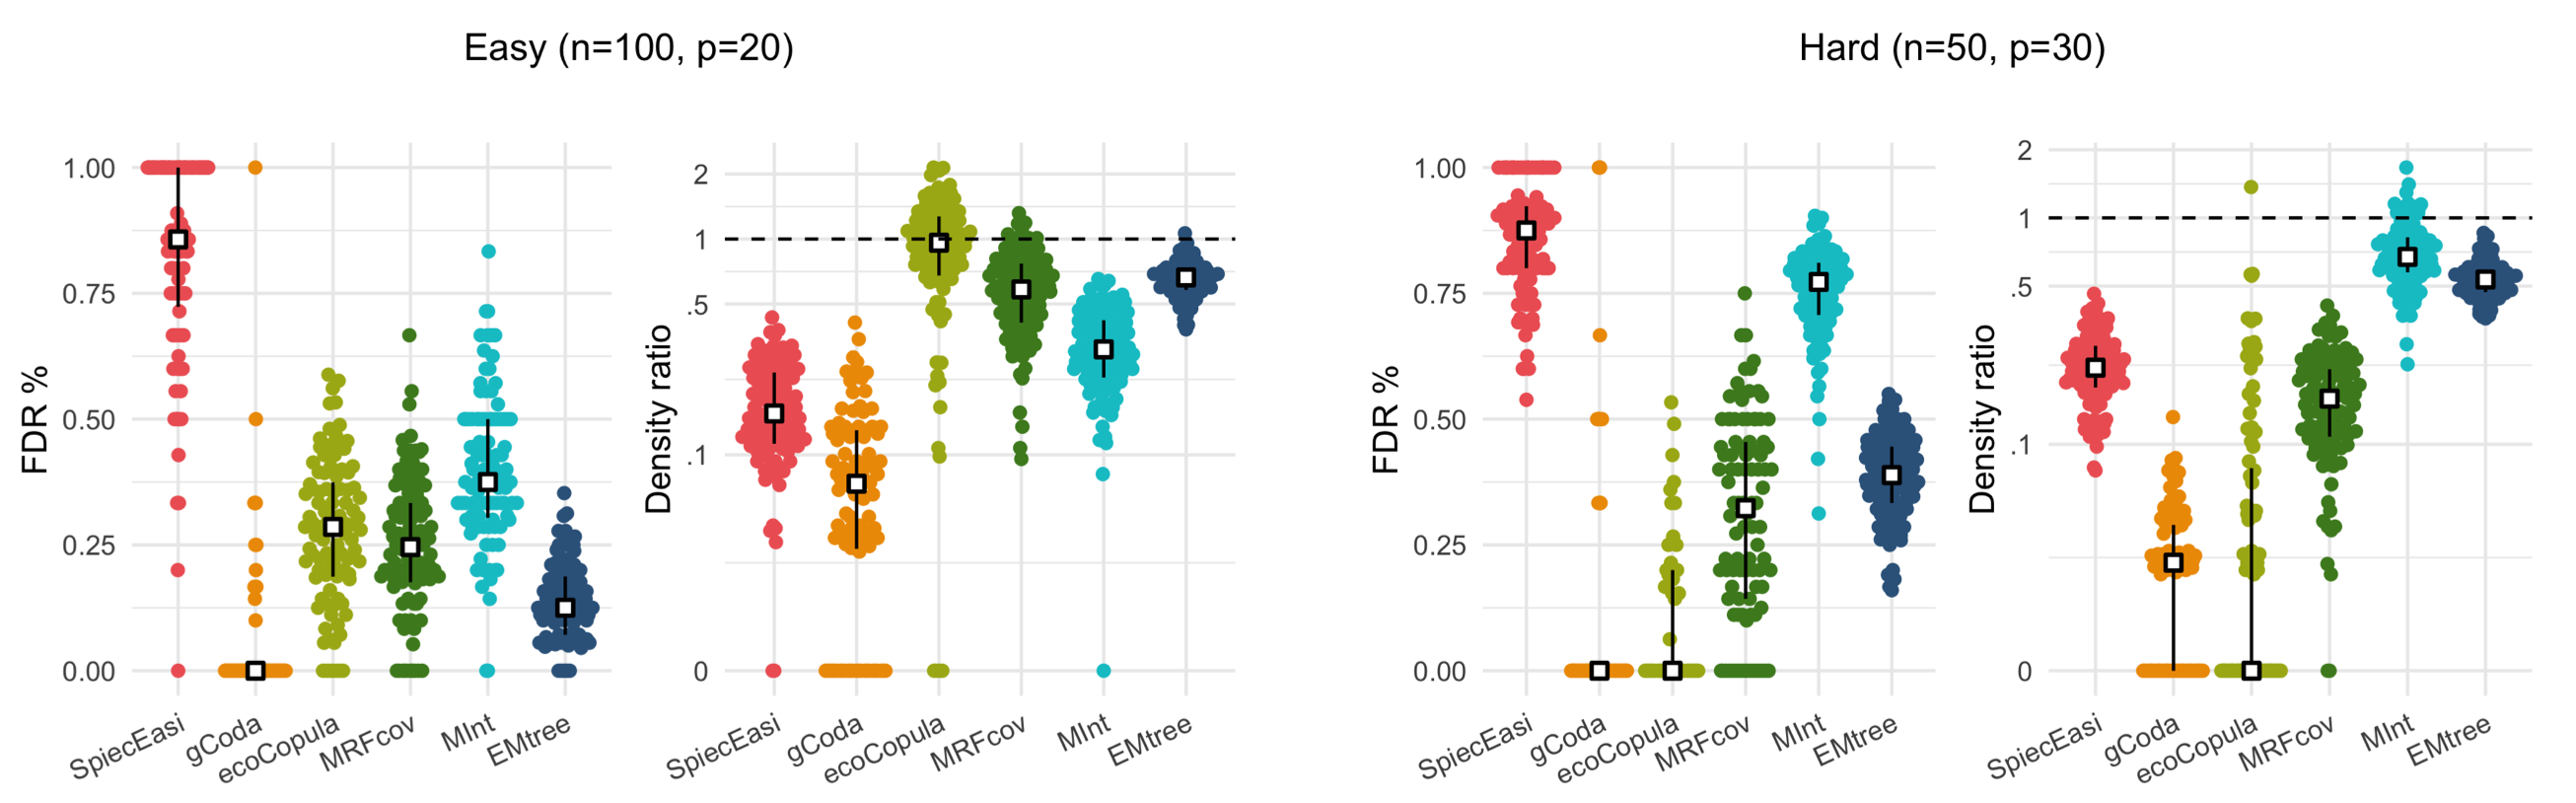
\includegraphics[width=\linewidth]{images/panel_erdos_6methods.png}\\
 \end{figure}
 \end{frame}
  \begin{frame}{Final networks comparison (Scale-free, more nodes)}
  \begin{figure}
 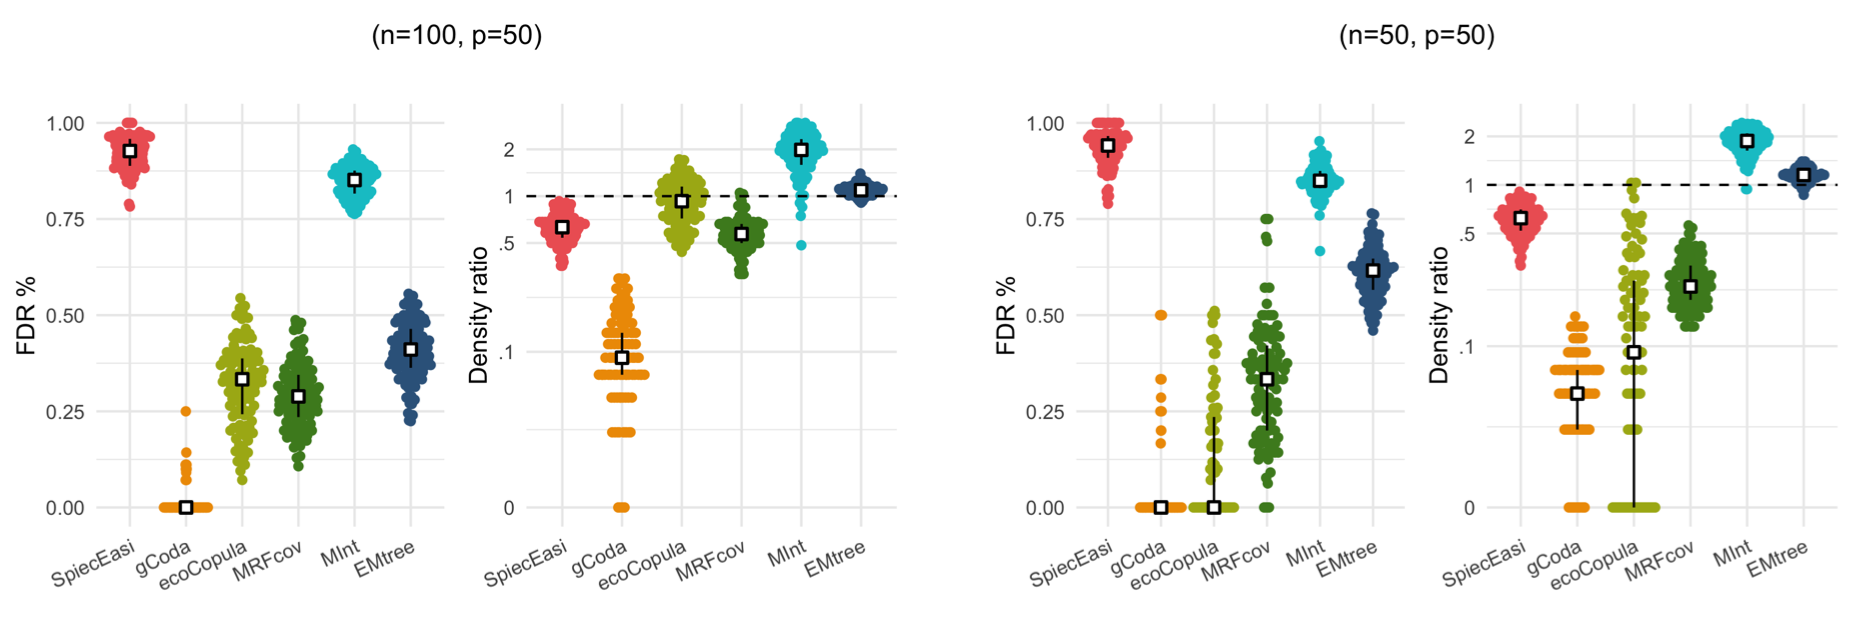
\includegraphics[width=\linewidth]{images/tpfn_sf.png}\\
 \end{figure}
 \small
 \begin{itemize}
 \item Thresholds for EMtree: $2/p$ for probabilities and then $80\%$ for the frequences.
 \item The optimal network of SpiecEasi is mostly wrong, whereas gCoda gives too sparse but right results
 \item EMtree is a good compromise. Higher thresholds would yield sparser results with less false positives.
 \end{itemize}
 \normalsize
 \end{frame}

 %=================================
 \begin{frame}{A study of threshold effects for a big network}
 \begin{itemize}
 \item Dependency structure: Erdös with 500 nodes, edge probability $3/p$
 \item EMtree on $S=30$ resamples
 \item Study the effect of the probability threshold on the frequencies performance
 \end{itemize}
    \begin{figure}
    \centering
 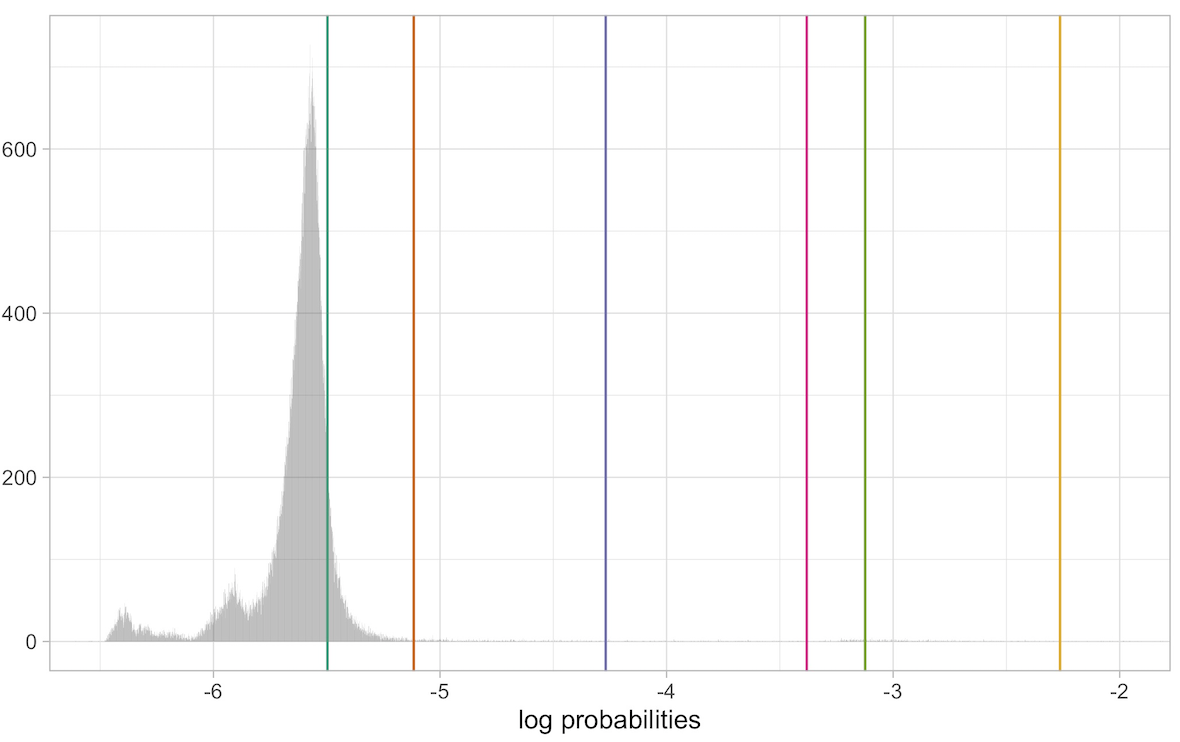
\includegraphics[width=0.6\linewidth]{images/prob_thresh.png}
 \caption{Threshold on $P$: $2/p+x$, $x\in \{10^{-4}, 2.10^{-3}, 10^{-2},3.10^{-2}, 4.10^{-2}, 0.1\}$}
   \end{figure}
 \end{frame}
  %====================================================================
 \begin{frame}{A study of threshold effects for a big network}
 PPV=1-FDR, TPR=TP/P
 \begin{figure}
 \centering
   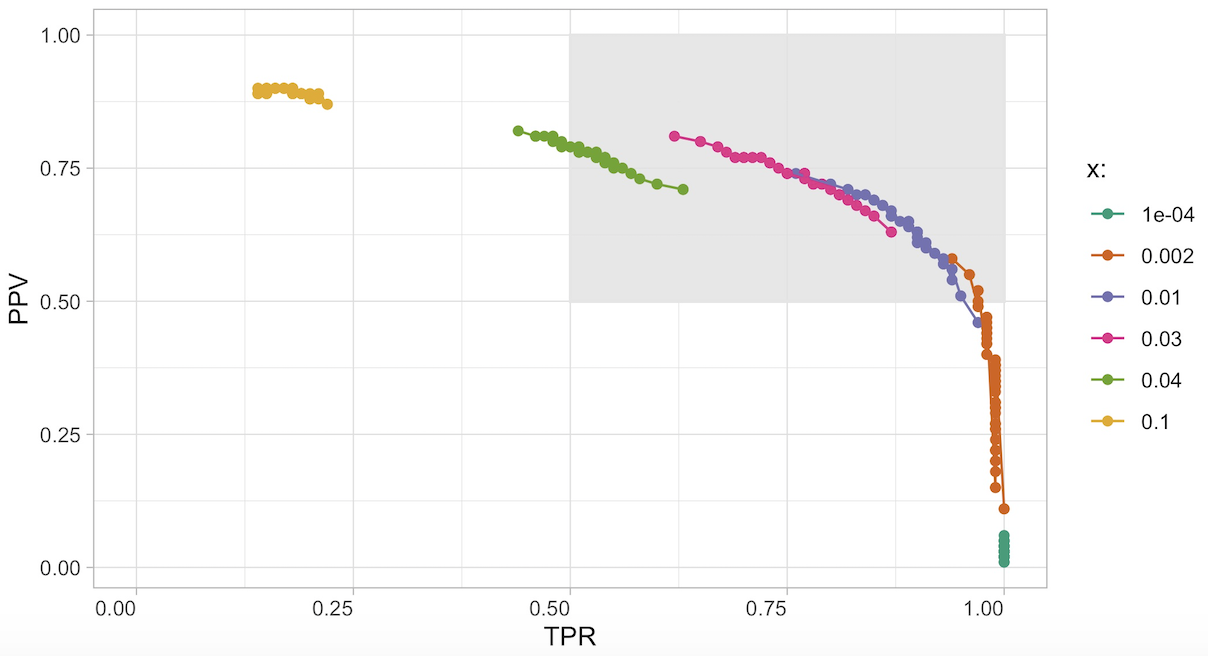
\includegraphics[width=10cm]{images/PPVTPR_500.png}
 \end{figure}
Choosing the first threshold is paramount, a model selection tool is under development.
 \end{frame}
  %====================================================================

%====================================================================
\subsection{Illustration}
\begin{frame}{Oak powdery mildew}
\begin{columns}
\begin{column}{5cm}
\begin{figure}[htp]
\centering
\includegraphics[scale=0.07]{images/EA.jpg}
\caption{\textit{Pathogen Erysiphe alphitoides (EA).}}
\end{figure}
\end{column}
\begin{column}{6cm}
\begin{figure}[htp]
\centering
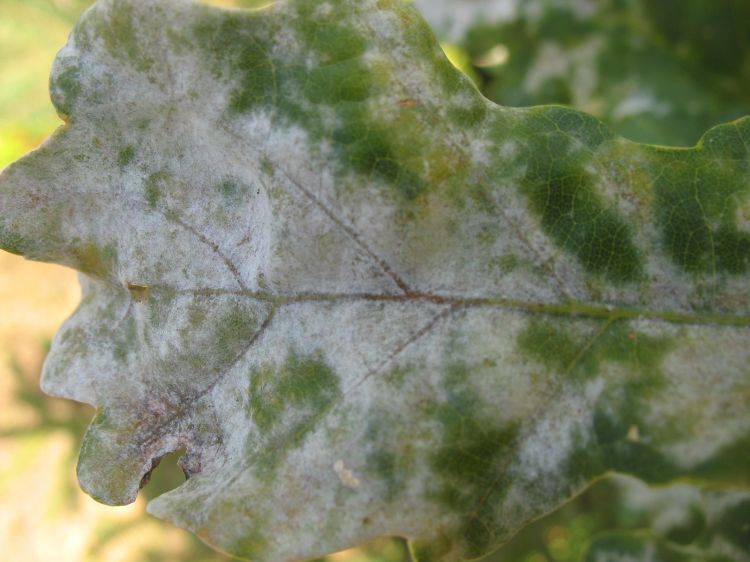
\includegraphics[scale=0.1]{images/mildew.jpg}
\caption{Oak leaf with powdery mildew.}
\end{figure}
\end{column}
\end{columns}
\vspace{0.5cm}
Metabarcoding of oak tree leaves microbiome \cite{jakuch}.\\

\begin{itemize}
	\item $\Ybf$: 116 sample of 114 microbial species counts (bacteria/fungi)
	\item $\Xb$: sampled tree, and 3 quantitative covariates 
	\item $\Ob$: Different read depth for bacteria and fungi
\end{itemize}
\end{frame}


%====================================================================
\begin{frame}{Oak mildew networks}
\begin{center}
\begin{figure}[htp]
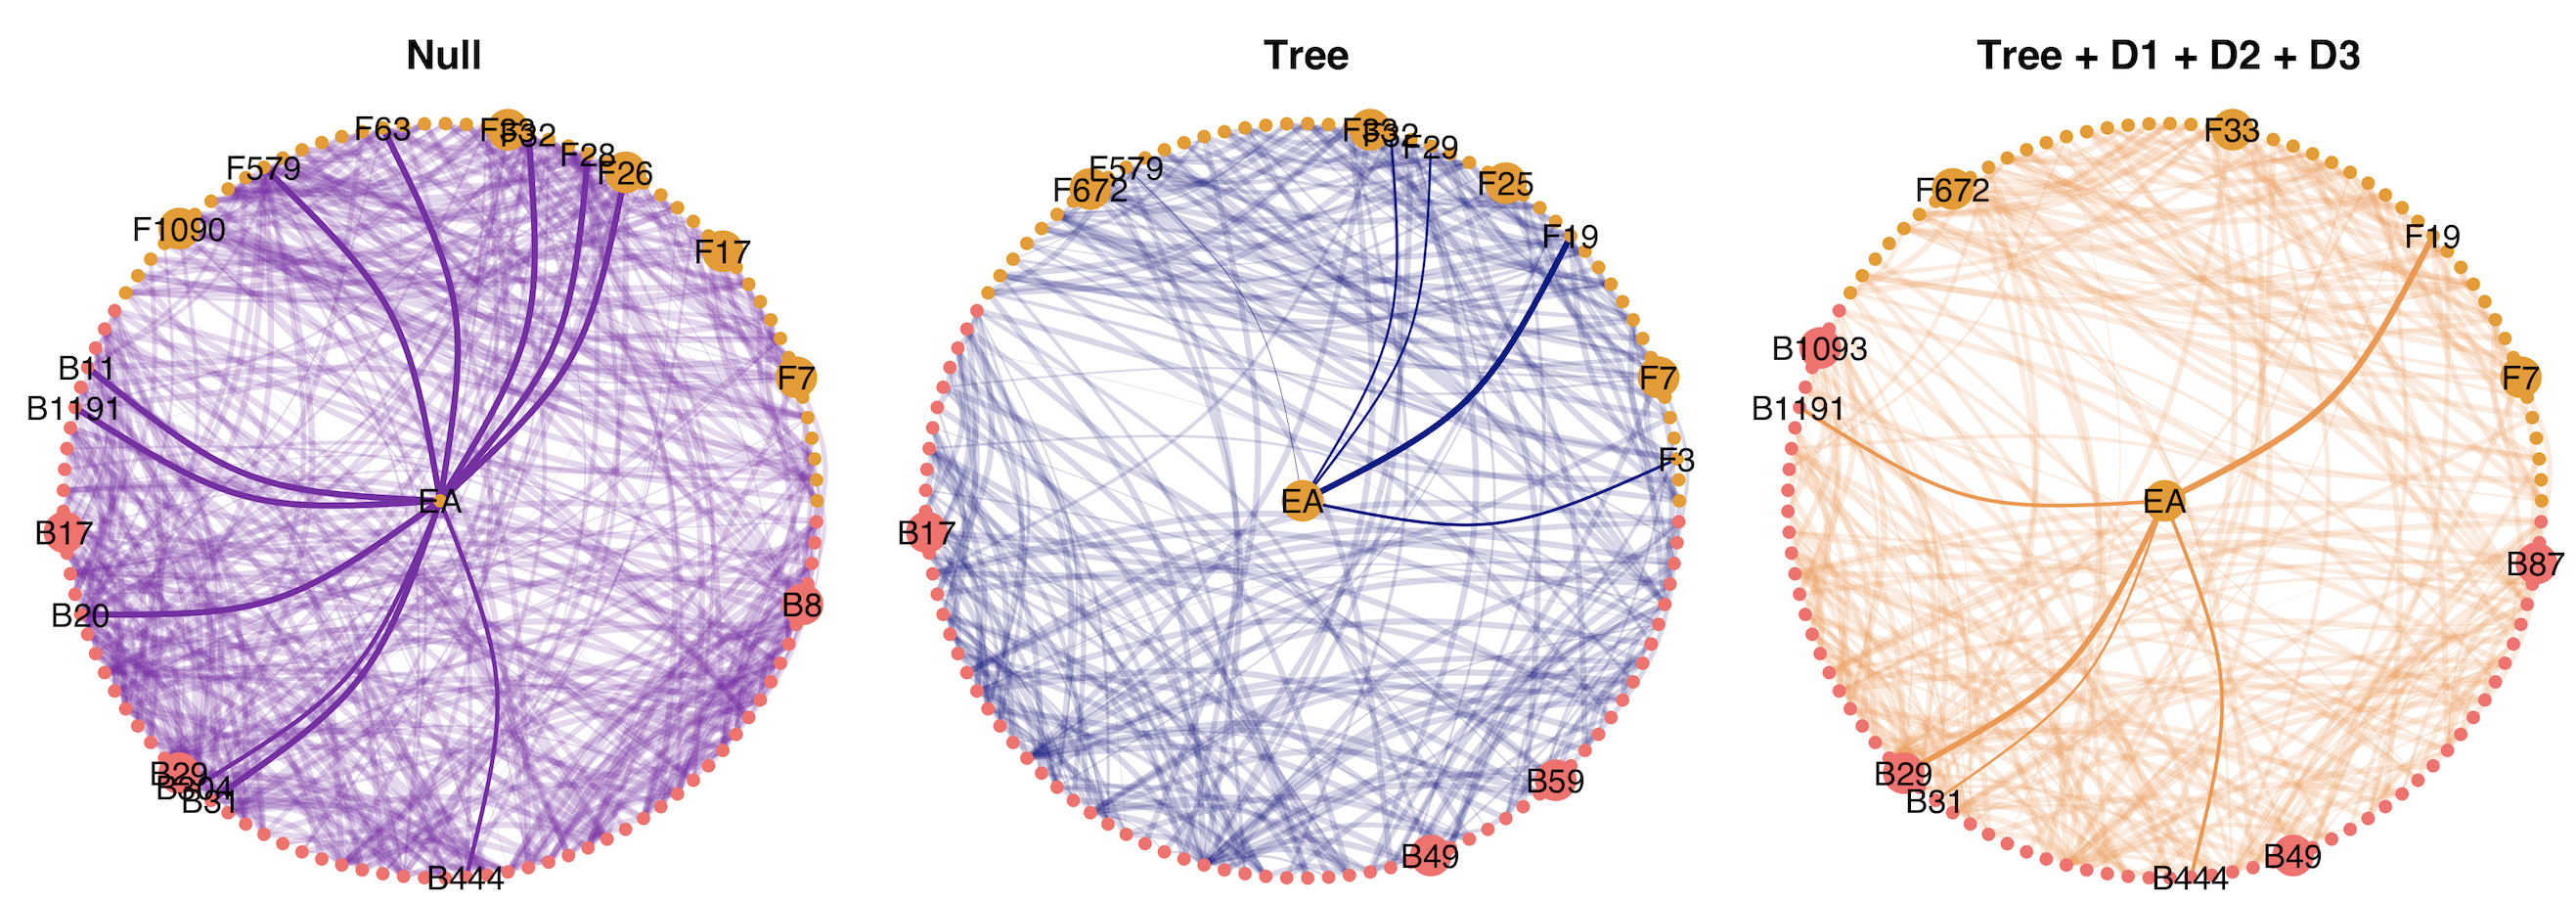
\includegraphics[width=\linewidth]{images/OakProbNets.png}
\end{figure}
\end{center}
\bigskip

\footnotesize{Frequencies above $90\%$.\\6.5s: average running time for one model.}\normalsize
\end{frame}
%====================================================================
\begin{frame}{Ea neighbors: previous study}
On the 39 infected samples:
\begin{figure}
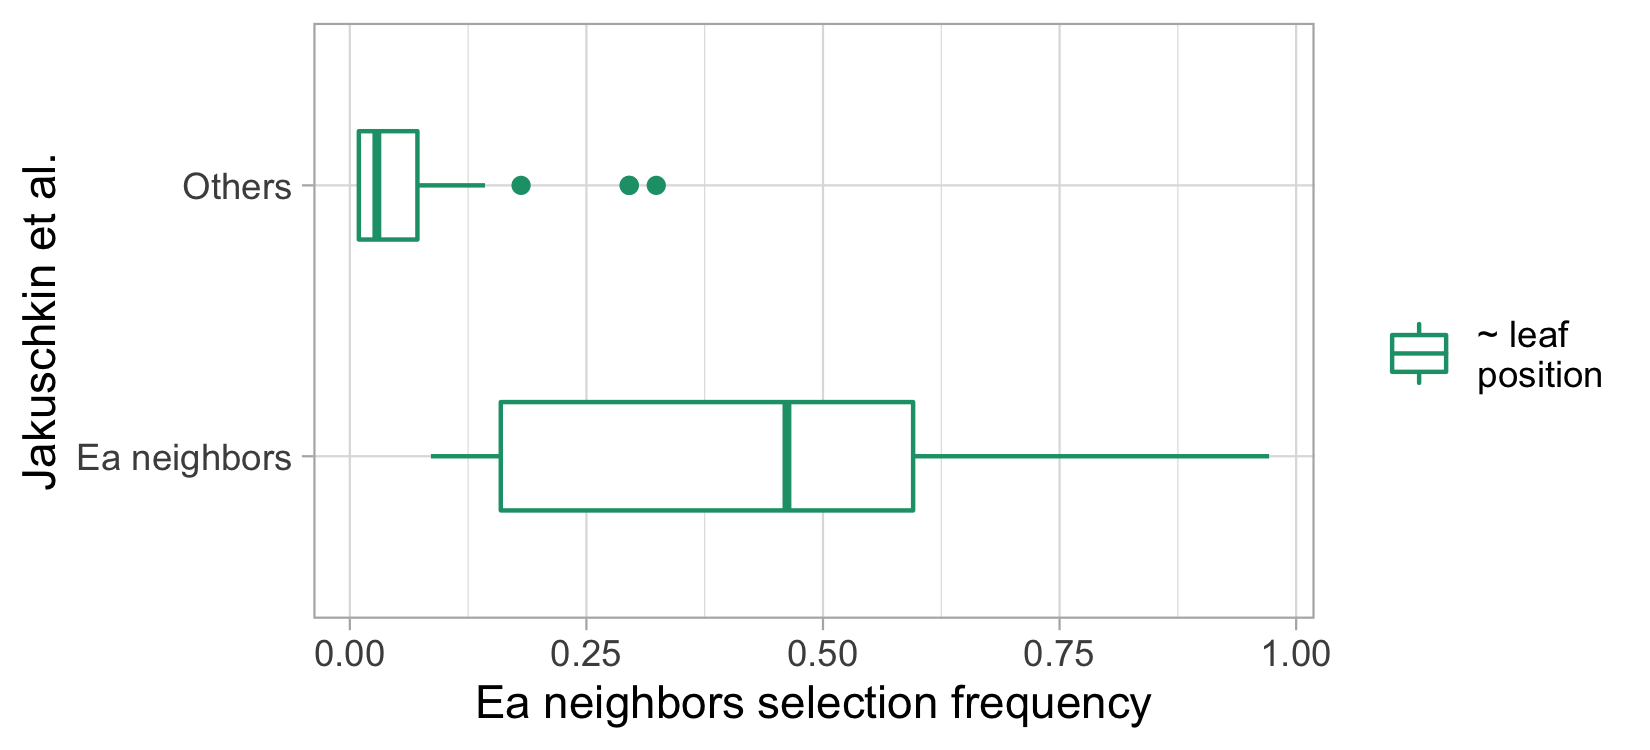
\includegraphics[width=0.8\linewidth]{images/EAneighbors.png}
\caption{Comparison with \citet{jakuch}}
\end{figure}
\footnotesize{20s: average running time.}\normalsize
\end{frame}
%====================================================================

 %%%%%%%%%%%%%%%%%%%%%%%%%%%%%%%%%%
%%%%%%%%%%%%%%%%%%%%%%%%%%%%%%%%%%
 
\section{Inference from incomplete counts}
\begin{frame}{}
\begin{center}
\Huge{\bleu{Inference from incomplete counts}}
\end{center}
\begin{center}
\begin{description}
\item[i] Model
\item[ii]  Inference
\item[iii] Illustration
\end{description}
\end{center}
\end{frame}
%====================================================================
\begin{frame}{Marginalization of graphs}
 \begin{columns} 
 \begin{column}{0.4\linewidth}
 \begin{flushright}
\begin{tabular}{c}
 {Complete graph:}\\\\
 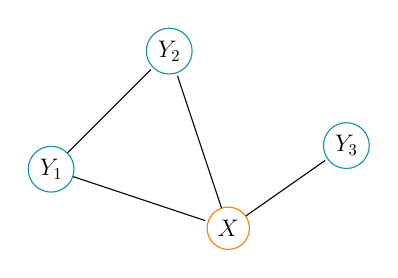
\begin{tikzpicture}
     
      \tikzstyle{every edge}=[-,>=stealth',shorten >=1pt,auto,thin,draw]
		\node[observed] (A1) at (0*\edgeunit, 0*\edgeunit) {$Y_1$};
	\node[bigMissing] (A2) at (1.5*\edgeunit, -0.5*\edgeunit) {
		$X$};
	
		\node[observed] (A3) at (1*\edgeunit, 1*\edgeunit) {$Y_2$};
		\node[observed] (A4) at (2.5*\edgeunit, 0.2*\edgeunit) {$Y_3$};
		\path (A1) edge [] (A2)
        (A1) edge [] (A3)
        (A2) edge [] (A3)
        (A2) edge [] (A4);
\end{tikzpicture}
\end{tabular}\\
 \end{flushright}
 \end{column}
 \begin{column}{0.1\linewidth}
\begin{center}
 $\Longrightarrow$
\end{center}
\end{column}
 \begin{column}{0.4\linewidth}
 \begin{flushleft}
\vspace{0.8cm}
\begin{tabular}{c}
  {Marginal graph}:\\\\
 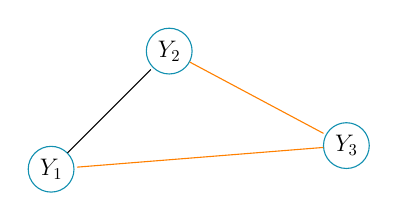
\begin{tikzpicture}
      \tikzstyle{every edge}=[-,>=stealth',shorten >=1pt,auto,thin,draw]
		\node[observed] (A1) at (0*\edgeunit, 0*\edgeunit) {$Y_1$};
		%\node[observed] (A2) at (1.5*\edgeunit, -0.5*\edgeunit) {$A_2$};
		\node[observed] (A3) at (1*\edgeunit, 1*\edgeunit) {$Y_2$};
		\node[observed] (A4) at (2.5*\edgeunit, 0.2*\edgeunit) {$Y_3$};
		\path  (A1) edge [] (A3)
        (A3) edge [orange] (A4)
        (A4) edge [orange] (A1);
\end{tikzpicture}
\end{tabular}\\
\end{flushleft}
Spurious edges leading to wrong interpretation\\
 \end{column}
\end{columns}
\bigskip

$X$ is a \emphase{missing actor}.
\end{frame}
%=======================================
\subsection{Model}
\begin{frame}{Added hidden Gaussian parameters}
\begin{columns}
 \begin{column}{0.4\linewidth}
  \begin{center}
	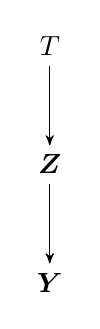
\begin{tikzpicture}	
      \tikzstyle{every edge}=[-,>=stealth',auto,thin,draw]
		\node (A1) at (0*\length, 2*\length) {$T$};
		\node (A2) at (0*\length, 1*\length) {$\Zbf$};
		\node (A3) at (0*\length, 0*\length) {$\Ybf$};
		\draw (A1) edge [->](A2);
        \draw (A2) edge [->] (A3);
	\end{tikzpicture} 
   \end{center}
   $$\Zbf\mid T\sim\Ncal(0,\Omegab_T^{-1})$$
 \end{column}
  \begin{column}{0.1\linewidth}
  $\Longrightarrow$
   \end{column}
     \begin{column}{0.5\linewidth}
     \begin{center}
	\begin{tikzpicture}	
      \tikzstyle{every edge}=[-,>=stealth',auto,thin,draw]
		\node (A1) at (0.625*\length, 2*\length) {$T$};
		\node (A2) at (0*\length, 1*\length) {\emphase{$\Zbf_O$}};
		\node (A3) at (1.25*\length, 1*\length) {\emphase{$\Zbf_H   $}};
		\node (A4) at (0*\length, 0*\length) {$\Ybf$};
		\draw (A1) edge [->](A2);
        \draw (A1) edge [->] (A3);
        \draw (A2) edge  (A3);
        \draw (A2) edge [->](A4);
	\end{tikzpicture} 
	  \end{center}
	     $$(\Zbf_O,\Zbf_H)\mid T\sim\Ncal(0,\Omegab_T^{-1})$$
   \end{column}
    \end{columns}
    \begin{columns}
    \begin{column}{0.5\linewidth}
      \vspace{0.2cm}
         
       \hspace{0.6cm}  $\Zbf$: $n\times p$\\
     \end{column}
         \begin{column}{0.5\linewidth}
         \vspace{0.3cm}
         
       \hspace{0.85cm}  $\Zbf_O$: $n\times p$\\
       \hspace{0.85cm}   \emphase{$\Zbf_H$: $n\times r$} \hspace{0.8cm} \emphase{$p'=p+r$.}
     \end{column}
     \end{columns}
     \vspace{0.2cm}
     \pause
     \begin{itemize}
     \item Same model with $r$ additional dimensions
     \item Need access to sufficient statistics regarding $Z_H$ 
     \end{itemize}
\end{frame}
%===========================================
%\begin{frame}{Conditional precision matrix}
%\begin{columns}
%\begin{column}{0.4\linewidth}
%\begin{align*}
% \Sigmab=
%  \left( {\begin{array}{cc}
%  \Omegab_{O} &  \Omegab_{OH}\\\\
%  \Omegab_{HO} & \Omegab_{H}
%  \end{array} } \right)^{-1} 
%  \end{align*}
%\end{column}
%\begin{column}{0.6\linewidth}
% Schur's complement in block-matrix inversion:
%  $$\Sigmab_O^{-1} = \Omegab_{O\mid H} = \Omegab_O-\Omegab_{OH}\Omegab_H^{-1}\Omegab_{HO}$$
%\end{column}
%\end{columns}
%
%\bigskip
%\bigskip
% 
%  Therefore:
%  $$(\Zbf_O,\Zbf_H)\sim\Ncal(0,\Omegab^{-1}) \Rightarrow \Zbf_O\sim\Ncal\left(0,(\Omegab_O\emphase{-\Omegab_{OH}\Omegab_H^{-1}\Omegab_{HO}})^{-1}\right)$$
%  
%  \vspace{0.2cm}
%  
%  \begin{center}
%  $\Rightarrow$ \emphase{Additional edges in the marginal network.}
%  \end{center}
%\end{frame}
%===============================
\subsection{Inference}
\begin{frame}{Variational EM algorithm}
\begin{columns}
\begin{column}{0.7\linewidth}
Finding  distribution  $\emphase{q(\Hb)}\approx p(\Hb\mid\Ybf)$:\\

\begin{itemize}
\item Restricting the search space to a family $Q$,
\item Choosing $q$ with smallest distance to $p(\Hb\mid\Ybf)$.\\
\end{itemize}
\end{column}
\begin{column}{0.25\linewidth}
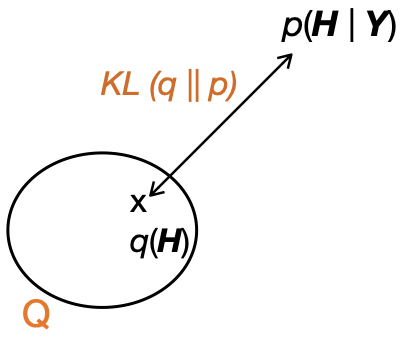
\includegraphics[width=3cm]{images/VEM.png}
\end{column}
\end{columns}
\bigskip

Doing so maximizes a lower-bound of the log-likelihood:
\begin{center}
$\J ( \Theta ; q) = \log p_{\Theta }(\Ybf)  - KL(q(\Hb) \mid\mid p_{\Theta }(\Hb\mid\Ybf)).$
\end{center}

\begin{block}{Variational EM algorithm}
\begin{description}
\item[VE step:] \small{$q^{t+1}=\argmax_{q\in Q } \big\{\J( \Theta^t ; q^t) \big\}$ $= \argmin_{q\in Q } \big\{KL(q^t\mid\mid p_{\Theta^t }) \big\} $}
\item[M step:]$\Theta^{t+1} = \argmax_{\Theta } \big\{\J( \Theta^t; q^{t+1}) \big\}$\normalsize
\end{description}
\end{block}
\end{frame}
%===============================
%\begin{frame}{A product form for $q$}
%\begin{block}{Mean-field approximation \citep{beal}}
%In a VEM with $K$ hidden variables $\Zbf=\{z_1,...,z_K\}$  using  the KL divergence, if $Q$ is the set of  product-form distributions then the following holds:
%$$\text{VE step: } q_k^{(t+1)}(z_k)  \propto \exp \left\{ \Esp_{q_{\setminus k}^t} \left[ \log p_{\thetabf^{t+1}}(\Ybf, \Zbf) \right] \right\}.$$
%\end{block}
%
%In our model, two hidden variables: $\Zbf=(\Zbf_O, \Zb_H)$ and $T$.
%\emphase{$$q(\Zbf, T) = h(\Zbf)\,g(T).$$}
%According to $q$, $h$ and $g$ are independent. 
%%This eases computations by allowing to separate expectations:
%%$$\Esp_{\emphase{q}}[f(\Zbf)\times f(T)] = \Esp_{\emphase{g}}[f(T)]\times \Esp_{\emphase{h}}[f(\Zbf)]$$
%\end{frame}
%===============================
\begin{frame}{Variational distribution}
 Two hidden variables: $\Zbf=(\Zbf_O, \Zb_H)$ and $T$.
\emphase{$$q(\Zbf, T) = h(\Zbf)\,g(T).$$}
\begin{description}
\item[$h(\Zbf)$:] Product (independence of samples $i$) of Gaussians: 
$$h(\Zbf) = \prod_i \emphase{\Ncal_{p+r}}(\Zbf_i; \widetilde{\mbf}_i,\widetilde{\sbf}_i)$$
\item[$g(T)$:] Mean-field approximation: $g(T) \propto \exp\{\Esp_h[\underbrace{\log p_\betabf ( T) + \log p_\Omegab(\Zbf\mid T)}_{\text{Factorizes on the edges of T}}]\}$
$$g(T)\propto \prod_{kl\in T} \betat_{kl}$$
\end{description}
\pause
\begin{equation*}
\begin{array}{rlll}
\text{Variational parameters: } &\emphase{\widetilde{\Mb}=(\widetilde{\Mb}_O, \widetilde{\Mb}_H)},& \emphase{\widetilde{\Sbf}=(\widetilde{\Sbf}_O, \widetilde{\Sbf}_H)}, &\emphase{\betabft}\\
&{ n\times p',} &n\times p', &p'^2
\end{array}
\end{equation*}
\end{frame}

%================================
\begin{frame}{Proposed algorithm}
\begin{description}
\item[PLNmodels: ] Parameters regarding the observed part: $\widehat{\thetab}$, $\widetilde{\Mb}_O$,$\widetilde{\Sbf}_O$\\
\begin{itemize}
\item Fixed for further computations.
\end{itemize}\vspace{0.5cm}
\item[VE step: ] Update variational parameters: $\widetilde{\Mb}_H^{t+1}$, $\widetilde{\Sbf}_H^{t+1}$, $\betabft^{t+1}$\\
\begin{itemize}
\item Given by shapes of $g$ and $h$ distributions.
\end{itemize}\vspace{0.5cm}

\item[M step: ] Update model parameters: $\Omegab_T^{t+1}$, $\betab^{t+1}$\\
\begin{itemize}
\item $\beta_{jk} = P_{jk}/ M(\betab)_{jk}$ with \footnotesize $P_{jk} = \sum_{T\in \mathcal{T}, T\ni jk} g(T)$,\\\normalsize
\item \only<1>{$\Omegab_T$: adaptation of ML estimators \citep{Lau96}.}
\only<2>{\emphase{$\Omegab_T$: adaptation of ML estimators} \citep{Lau96}.\\
$p'^{p'-2}\times p'^2/2$ parameters $\Rightarrow$ \emphase{$p'^2/2$ estimators}.}
\end{itemize}
\end{description}
 \end{frame}
 %================================
%\begin{frame}{Estimation of $\Omegab$}
%$$\Omegab= \argmax_\Omegab \Esp_{gh} [\log p_\Omegab(\Zbf\mid T)]$$
%For a specific tree:
%$$\Esp_h[\log p(\Zbf\mid T)] = \frac{n}{2}\log |\Omegab_T| - \frac{1}{2}tr(\Omegab_T\; SSD) + cst,$$
%where $SSD$ is a sufficient statistic:
%$$SSD =  \Esp_h[\Zbf^\intercal \Zbf] =\Mb^\intercal \Mb + \sum_i \Sbf_i .$$
%\end{frame}

  %================================
 \begin{frame}{Lauritzen's ML estimator}
 In a GGM with a \emphase{chordal} graph $\Gb$ (cliques $\Ccal$, separators $\Scal$ with multiplicities $\nu(S)$),  $SSD$ the sum of  squares matrix. \vspace{0.3cm}
 \begin{block}{General Lauritzen's MLE}
 $$\widehat{\Omegab}_\Gb^{MLE} = n\big(\sum_{C\in\Ccal} [(SSD_C)^{-1}]^{p'} - \sum_{S\in\Scal} \nu(S)[(SSD_S)^{-1}]^{p'}\big)$$
 \end{block}
 \only<1>{
 \begin{itemize}
 \item The general $SSD$ matrix do not depend on $\Gb$.
 \item The estimator uses $SSD$ according to the graph structure.
 \end{itemize}}
 \only<2>{\vspace{0.3cm}
 If $\Gb$ is a tree $T\in \mathcal{T}$:
 \begin{itemize}
 \item $T$ is chordal.
 \item Cliques are edges:  inverses of $2\times 2$ matrices.
 \item Separators are nodes: $\Scal = \{1,...,p'\}$.
 \item $\nu(k) = deg(k)-1$.
 \end{itemize}}

 \end{frame}
  %================================
  \begin{frame}{Update of $\Omegab_T$}
  We define:
  $$SSD =  \Esp_h[\Zbf^\intercal \Zbf \mid \Ybf] =\widetilde{\Mb}^\intercal \widetilde{\Mb} + diag(\sum_i \widetilde{\sbf}_i) .$$
  Tree simplification of Lauritzen's formula:
  \begin{align*}
 \emphase{ \omega_{Tjk}^{t+1}} &=  \emphase{ \mathds{1}\{jk\in T\}\left(\frac{-ssd_{jk}^t/n}{1-(ssd_{jk}^t/n)^2}\right) }, \\
   \omega_{Tkk}^{t+1} &=1-\sum_{j}  (ssd_{jk}^t/n)\times\omega_{Tjk}^{t+1} .
  \end{align*}
  The estimates \emphase{$\omega_{Tjk}$ are common to all trees} sharing the edge $jk$: estimating $\{\Omegab_T, T\in\mathcal{T}\}$ amounts to estimating $p'^2/2$ quantities.
  \end{frame}
  %================================
  \subsection{Illustration}
  \begin{frame}{Barent's sea fishes}
\begin{columns}
\begin{column}{0.5\linewidth}
\begin{itemize}
\item $\Ybf$: abundances of 30 fish species in 89 sites,\vspace{0.2cm}
\item $\Xb$: latitude, longitude, depth and temperature,
\item $\Ob$: total detections per site.
\end{itemize}
\end{column}
\begin{column}{0.5\linewidth}
\begin{figure}
  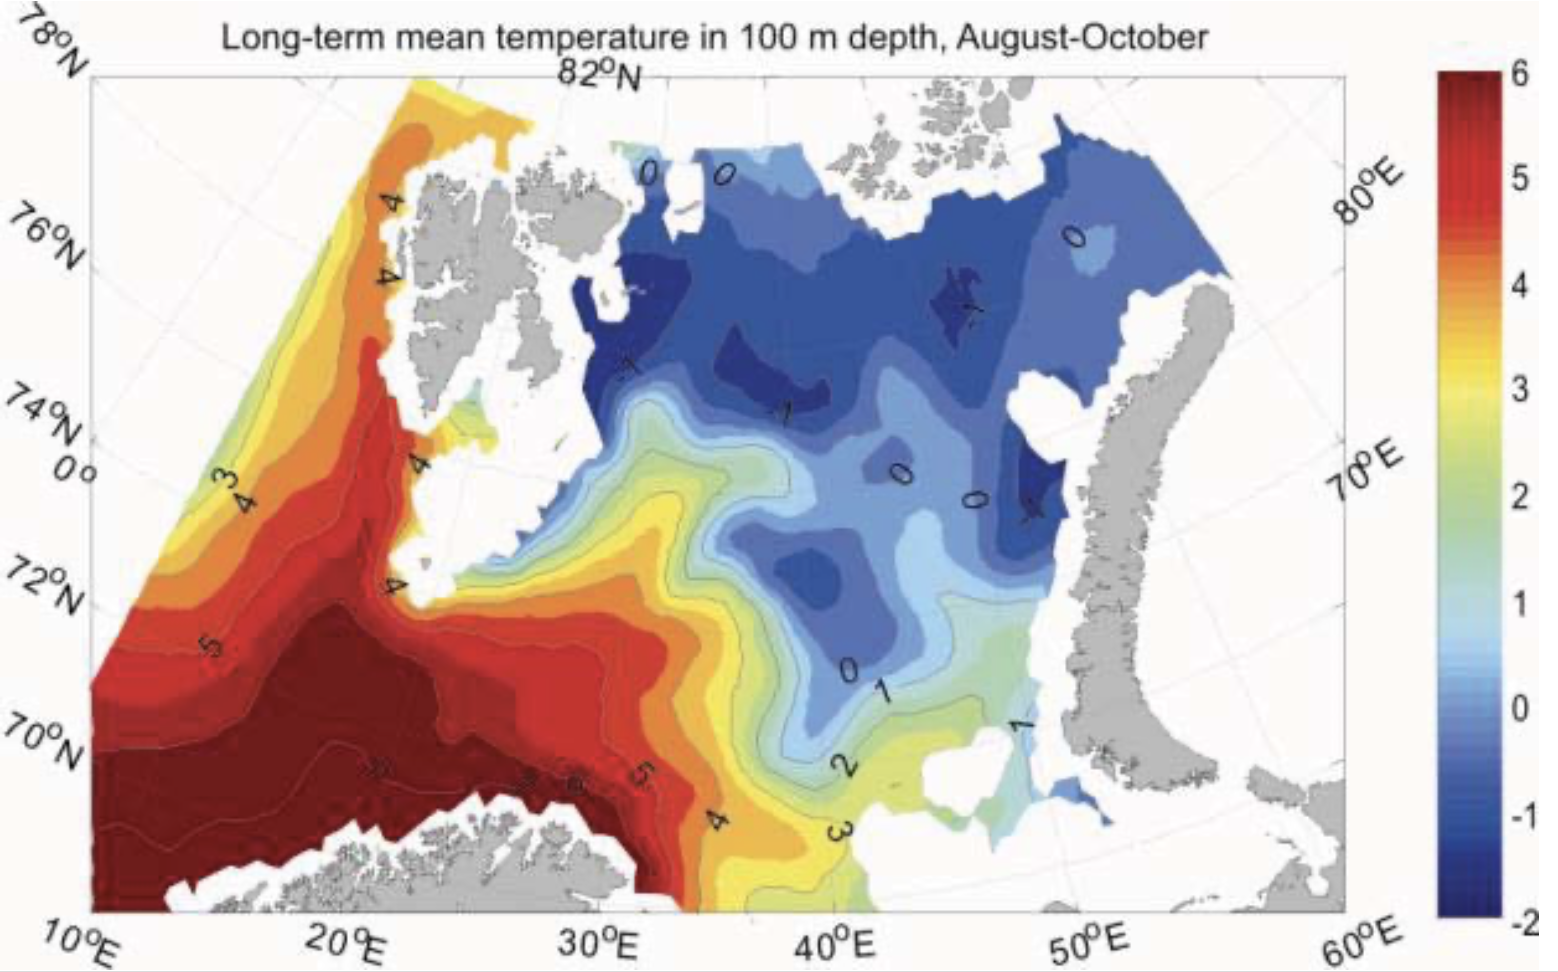
\includegraphics[width=6cm]{images/temp.png}
  \caption{\scriptsize{\citet{SEK09}}}\normalsize
  \end{figure}
\end{column}
\end{columns}
\begin{center}
  $\Rightarrow$ Fit with  no covariates.
  \end{center}
    \end{frame}
   
  %================================
    \begin{frame}{Barent's fishes networks}
  \begin{figure}
  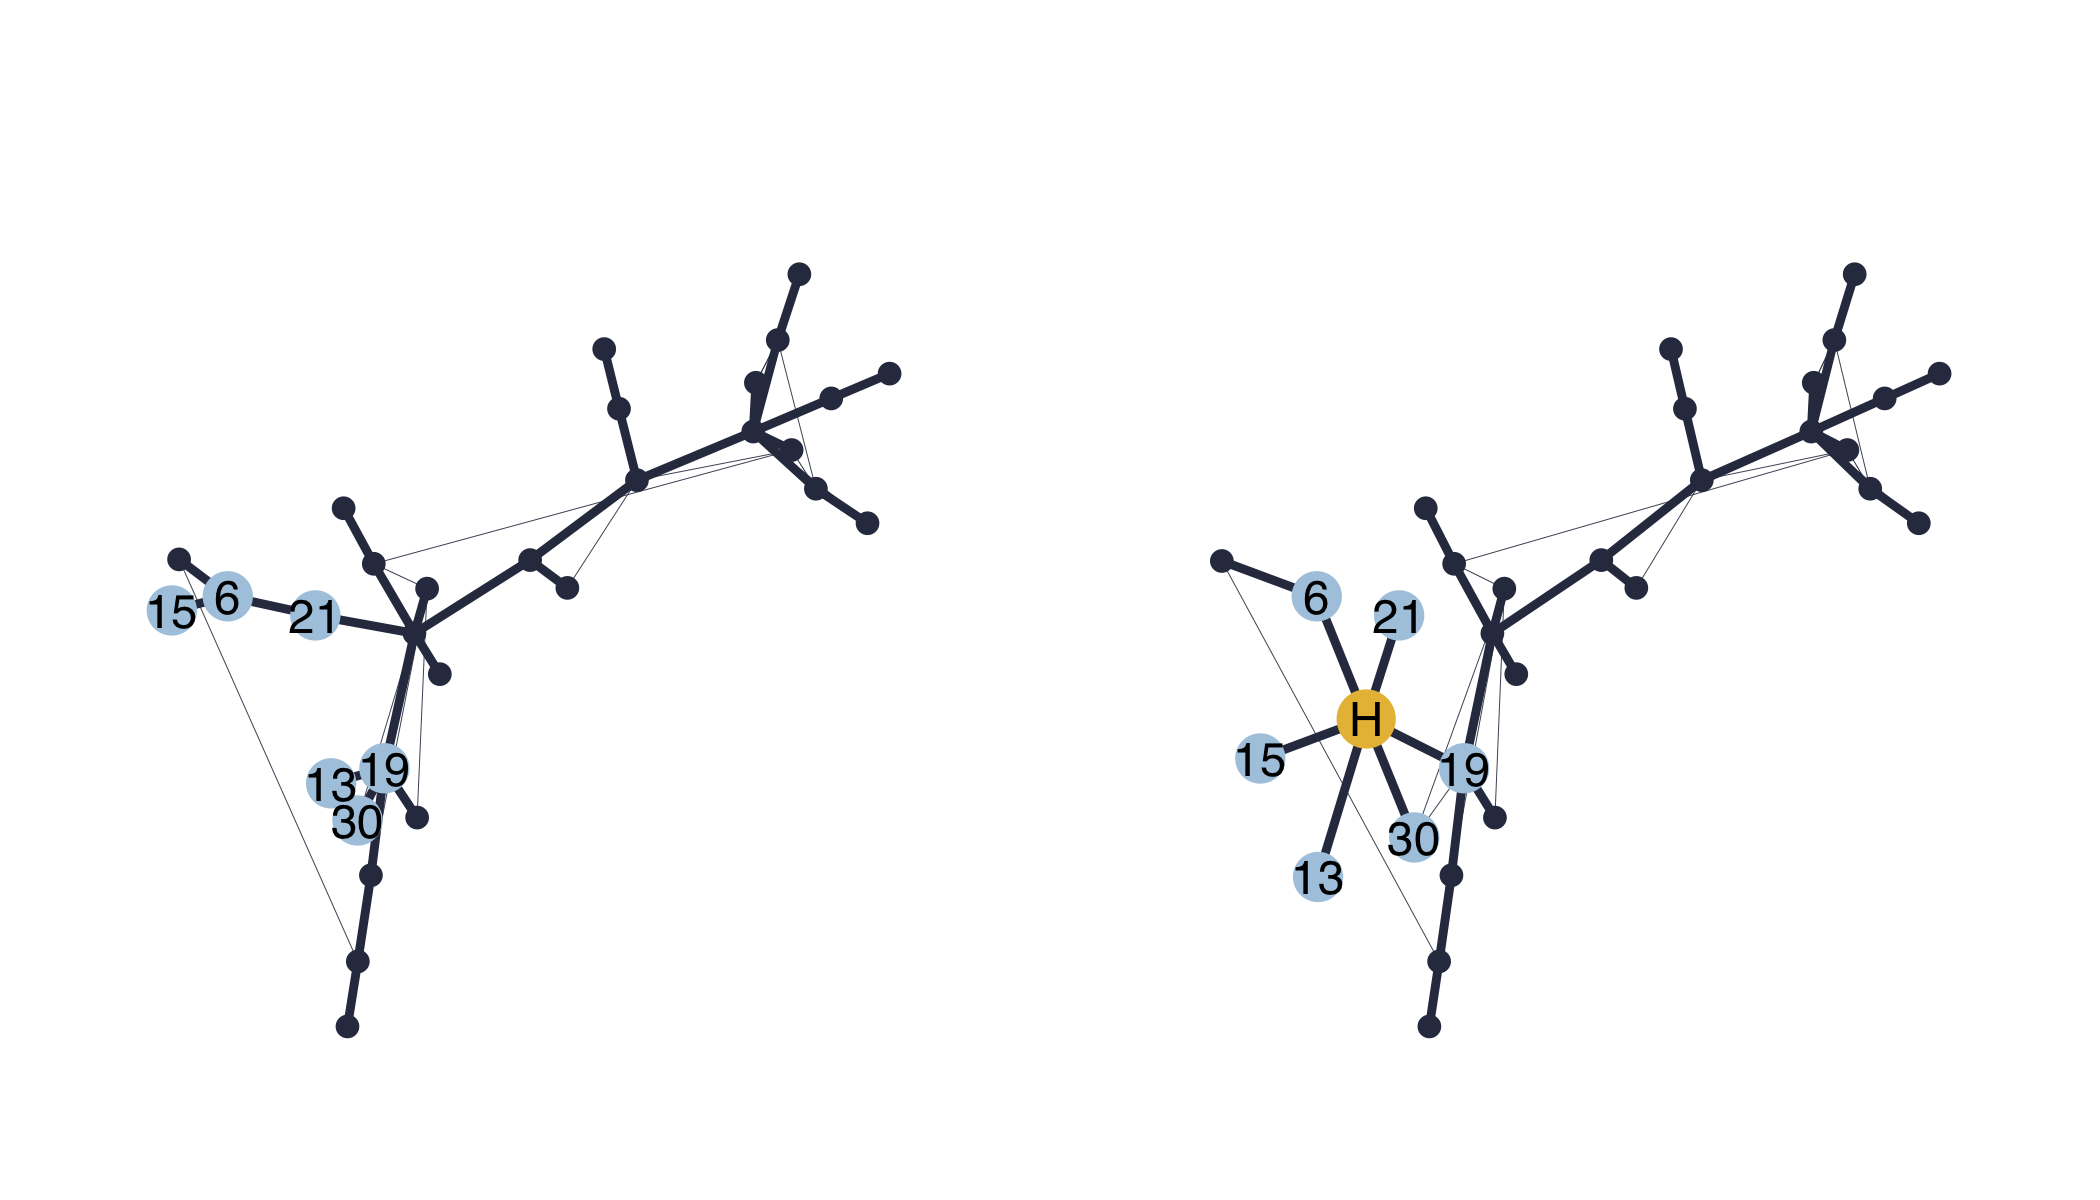
\includegraphics[width=0.9\linewidth]{images/Barents_net.png}
  \caption{\textit{Left}: observed network (3.3 mins). \textit{Right}: network inferred with one missing actor: H (5.0 mins).}
  \end{figure}
  \end{frame}
  %================================
    \begin{frame}{Relationship with temperature}
 
  \begin{columns}
\begin{column}{0.5\linewidth}
\begin{figure}
  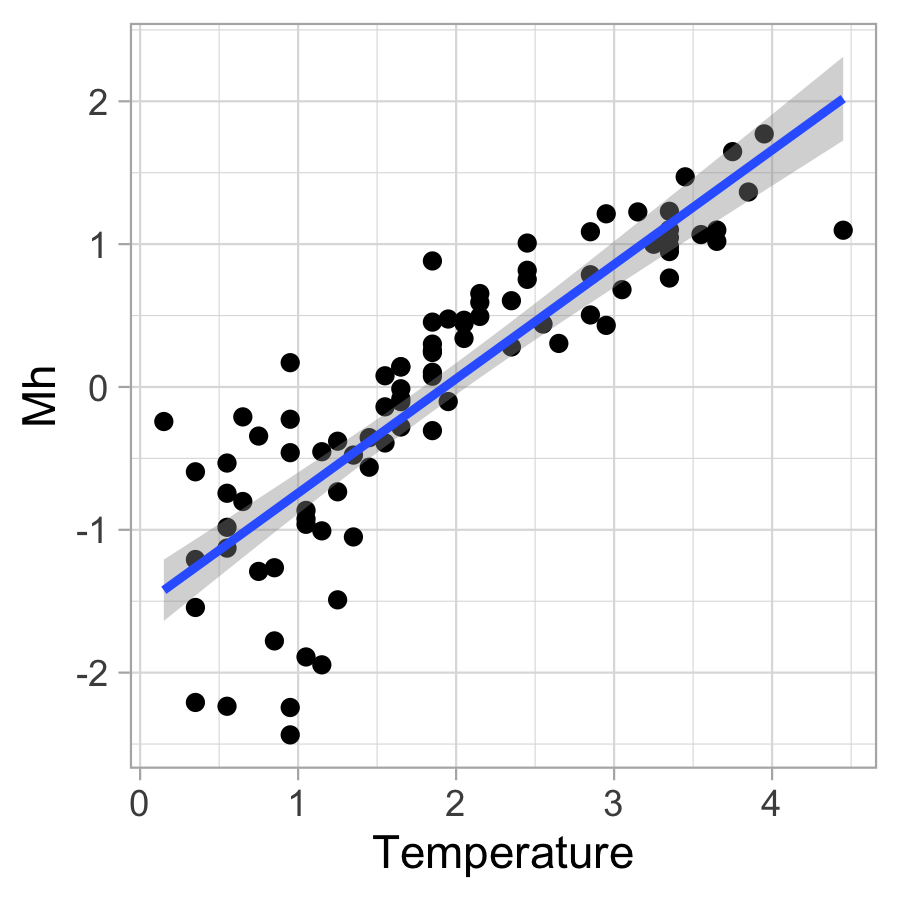
\includegraphics[width=0.9\linewidth]{images/Barents_MH.png}
  \caption{$Cor(Mh, Temp)=0.85$ .}
  \end{figure}
  \end{column}
  \begin{column}{0.5\linewidth}
  \begin{figure}
  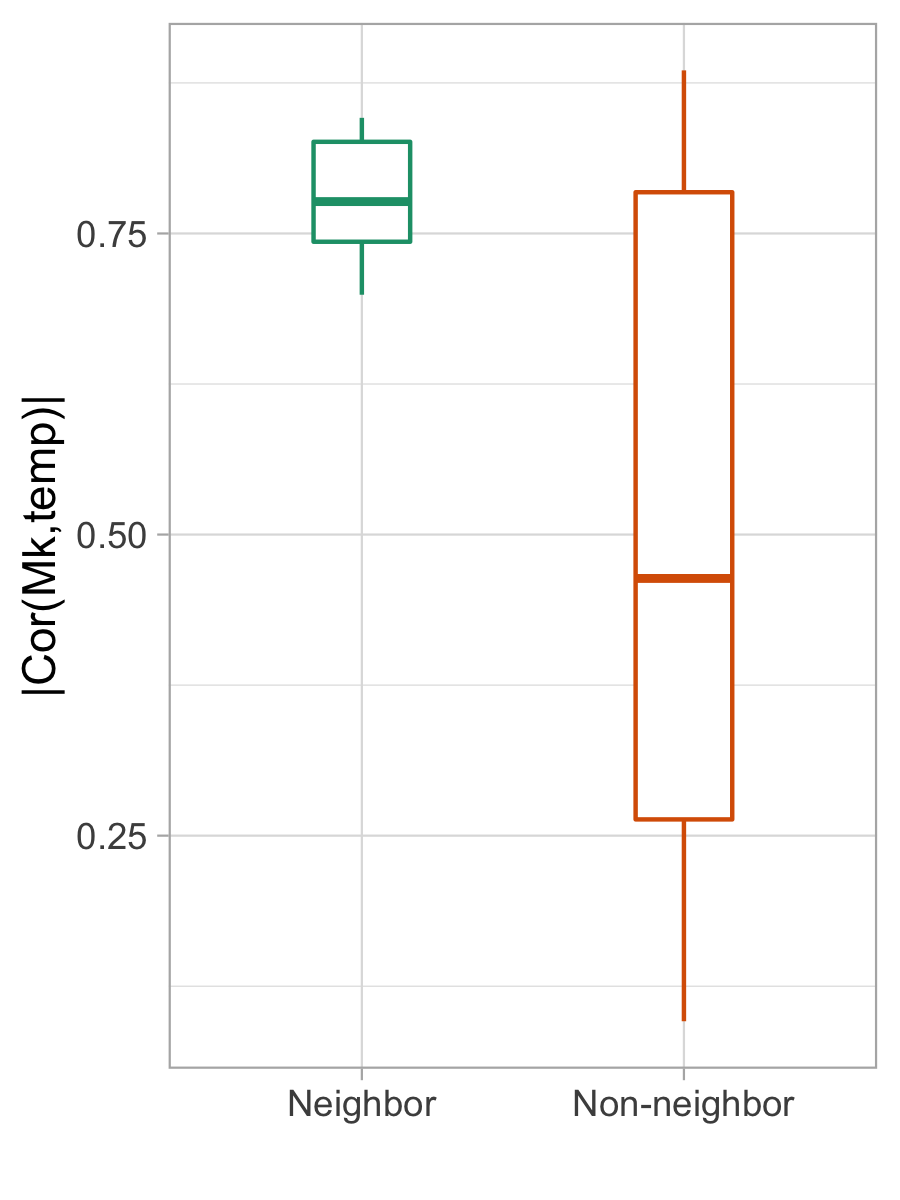
\includegraphics[width=0.6\linewidth]{images/Barents_neighb_cor.png}
  \caption{Direct neighbors are more linked to the temperature than other species.}
  \end{figure}
  \end{column}
  \end{columns}
  \end{frame}
  %================================
 

   %%%%%%%%%%%%%%%%%%%%%%%%%%%%%%%%%%
%%%%%%%%%%%%%%%%%%%%%%%%%%%%%%%%%%
 
\section{Perspectives}
\begin{frame}{}
\begin{center}
\Huge{\bleu{Conclusion and Perspectives}}
\end{center}
\begin{center}
%\begin{description}
%\item[i] Model
%\item[ii]  Inference
%\item[iii] Illustration
%\end{description}
\end{center}
\end{frame}

 %================================
 \begin{frame}{Conclusion}
 A probabilistic model for:\\
 
 
 \begin{itemize}
 \item Inferring conditional dependency network from abundance data.
 \item Accounting for covariates, offsets and missing actors.
  \end{itemize}
  \bigskip
  
  An inference which:\\
  
 \begin{itemize}
   \item Takes advantage of the Gaussian framework flexibility
 \item Uses spanning trees algebraic properties to rely on determinants and inverses of graph Laplacian matrices.
 \end{itemize}
  \bigskip
  
 Methods are implemented in R and available.
 \end{frame}
 
 %================================
% \begin{frame}{Extensions}
% \begin{description}
%\item[Tree averaging:]\begin{itemize}
%\item[]
%\item Requires a Gaussian layer:  possible with another emission law.
%\item Estimates a tree distribution: could be used for network comparison.
%\item Would allow network inference from observed counts directly.
%\end{itemize}
%\item[Gaussian layer:] \begin{itemize}
%\item[]
%\item Design a covariance structure accounting for spatial dependencies.
%\end{itemize}
%\item[Lauritzen's MLE:] \begin{itemize}
%\item[] 
%\item Get partial correlations to make interactions sign and strength available.
%\end{itemize}
%\end{description}
% \end{frame}
 %================================
 \begin{frame}{Extensions}
 \begin{description}
 \item[Network analysis:] \begin{itemize}
\item[]
\item Compare networks with the estimated tree distributions.
\item Study interactions sign and strength available by computing partial correlations.
\end{itemize}
\item[Ecological specifics:]\begin{itemize}
\item[]
\item Different emission law (presence/absence), provided there is a Gaussian latent layer of parameters.
\item Account for spatial dependencies within the Gaussian covariance structure.
\end{itemize}
\item[Direct model:] \begin{itemize}
\item[] 
\item Graphical model on counts with tree averaging

\end{itemize}
\end{description}
 \end{frame}
 
 %================================
 \begin{frame}{Contributions}
\begin{description}
\item[Articles] \begin{itemize}
\item[]\vspace{-0.5cm}\small
\item Momal R.,  Robin S., and Ambroise C. . \textit{"Tree‐based inference of species interaction networks from abundance data."} Methods in Ecology and Evolution 11.5 (2020): 621-632.\vspace{0.2cm}
\item  Momal R.,  Robin S., and Ambroise C. . \textit{"Accounting for missing actors in interaction network inference from abundance data."}  arXiv preprint arXiv:2007.14299 (2020).
\end{itemize}\vspace{0.5cm}
\item[R packages] \begin{itemize}
\item[]\vspace{-0.5cm}\normalsize
\item \texttt{EMtree}: \url{https://rmomal.github.io/EMtree/}.\vspace{0.2cm}
\item \texttt{nestor} \small(Network inference from Species counTs with missing actORs): \normalsize \url{https://rmomal.github.io/nestor}.
\end{itemize}
\end{description}  
\end{frame}
%%%%%%%%%%%%%%%%%%%%%%%%%%%%%%%%%%
%%%%%%%%%%%%%%%%%%%%%%%%%%%%%%%%%%
%%%%%%%%%%%%%%%%%%%%%%%%%%%%%%%%%%


\appendix
\backupbegin
\begin{frame}[allowframebreaks]
\bibliographystyle{apalike}
{\tiny
    \bibliography{biblio}}
\frametitle{References}
%\bibliography{cellcite}
\end{frame}

 %================================
 
 \section{Perspectives}
 \subsection{Network analysis}
 
   \begin{frame}{Signs and strengths of interactions}
        \only<1>{
       \scriptsize
   \begin{columns}
    \begin{column}{0.6\linewidth}
      $$\rho_{jk} = \frac{-\omega_{jk}}{\sqrt{\omega_{kk} \omega_{jj}}}$$
      $S$: sample covariance matrix of $\Zbf$. \\
      $\widehat{S}$: fitted covariance matrix (\texttt{ggm} R package)
     \begin{figure}

 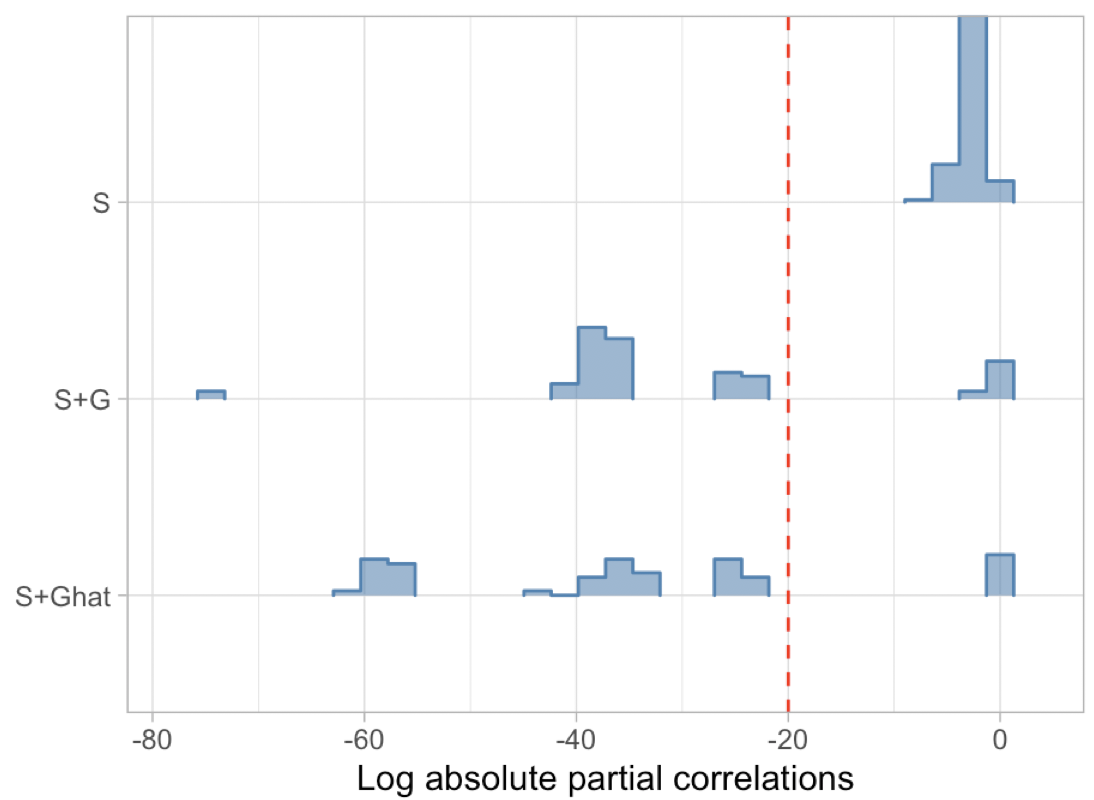
\includegraphics[width=\linewidth]{images/SG.png}
    
 \end{figure}
    \end{column}
      \begin{column}{0.3\linewidth}

      $\widehat{S} =S$:
      \begin{table}[ht]
\centering
\begin{tabular}{r|rrr}

 & -1 & 0 & 1 \\ 
  \hline
-1 &   5 &  45 &   0 \\ 
  1 &   0 &  48 &   7 \\ 

\end{tabular}
\end{table}
$\widehat{S} =f(S,\Gb)$:
\begin{table}[ht]
\centering
\begin{tabular}{r|rrr}

 & -1 & 0 & 1 \\ 
  \hline
-1 &   5 &   0 &   0 \\ 
  0 &   0 &  93 &   0 \\ 
  1 &   0 &   0 &   7 \\ 

\end{tabular}
\end{table}
$\widehat{S} =f(S,\widehat{\Gb})$:
\begin{table}[ht]
\centering
\begin{tabular}{r|rrr}

 & -1 & 0 & 1 \\ 
  \hline
-1 &   4 &   0 &   0 \\ 
  0 &   1 &  93 &   2 \\ 
  1 &   0 &   0 &   5 \\ 

\end{tabular}
\end{table}
     \end{column}
  \end{columns}}
    \only<2>{
    \begin{figure}
    \centering
     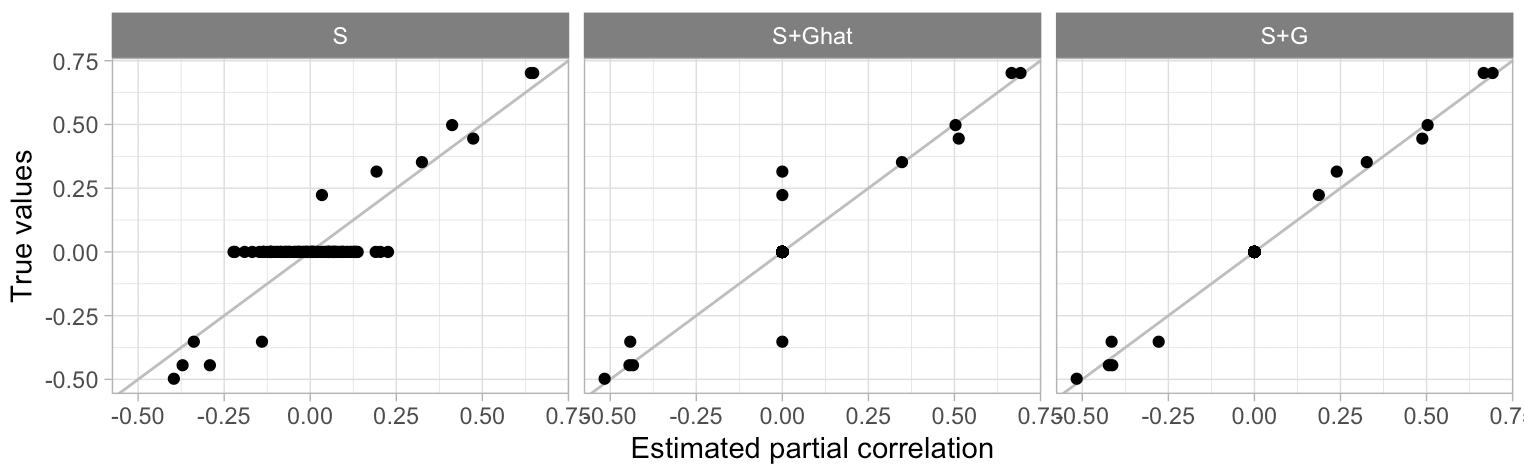
\includegraphics[width=\linewidth]{images/pcvalues.png}
    \end{figure}
         }
          
 \end{frame}
 %========================================
 \begin{frame}{Network comparison}
 \small
 \begin{align*}
 D(p_{\betabf^A}, p_{\betabf^B}) &=\frac{1}{2} \left[KL\big( p_{\betabf^B} \mid\mid p_{\betabf^A}\big)+KL\big( p_{\betabf^A}\mid\mid p_{\betabf^B} \big)\right]\\
 &= \sum_{kl} \log(\beta_{kl}^A/\beta_{kl}^B) \Big(\frac{P_{kl}^A - P_{kl}^B}{2}\Big)
 \end{align*}
 \bigskip
 
 \bleu{Oak dataset:}\\
 \vspace{0.3cm}
 
 \begin{columns}
  \begin{column}{0.5\linewidth}
  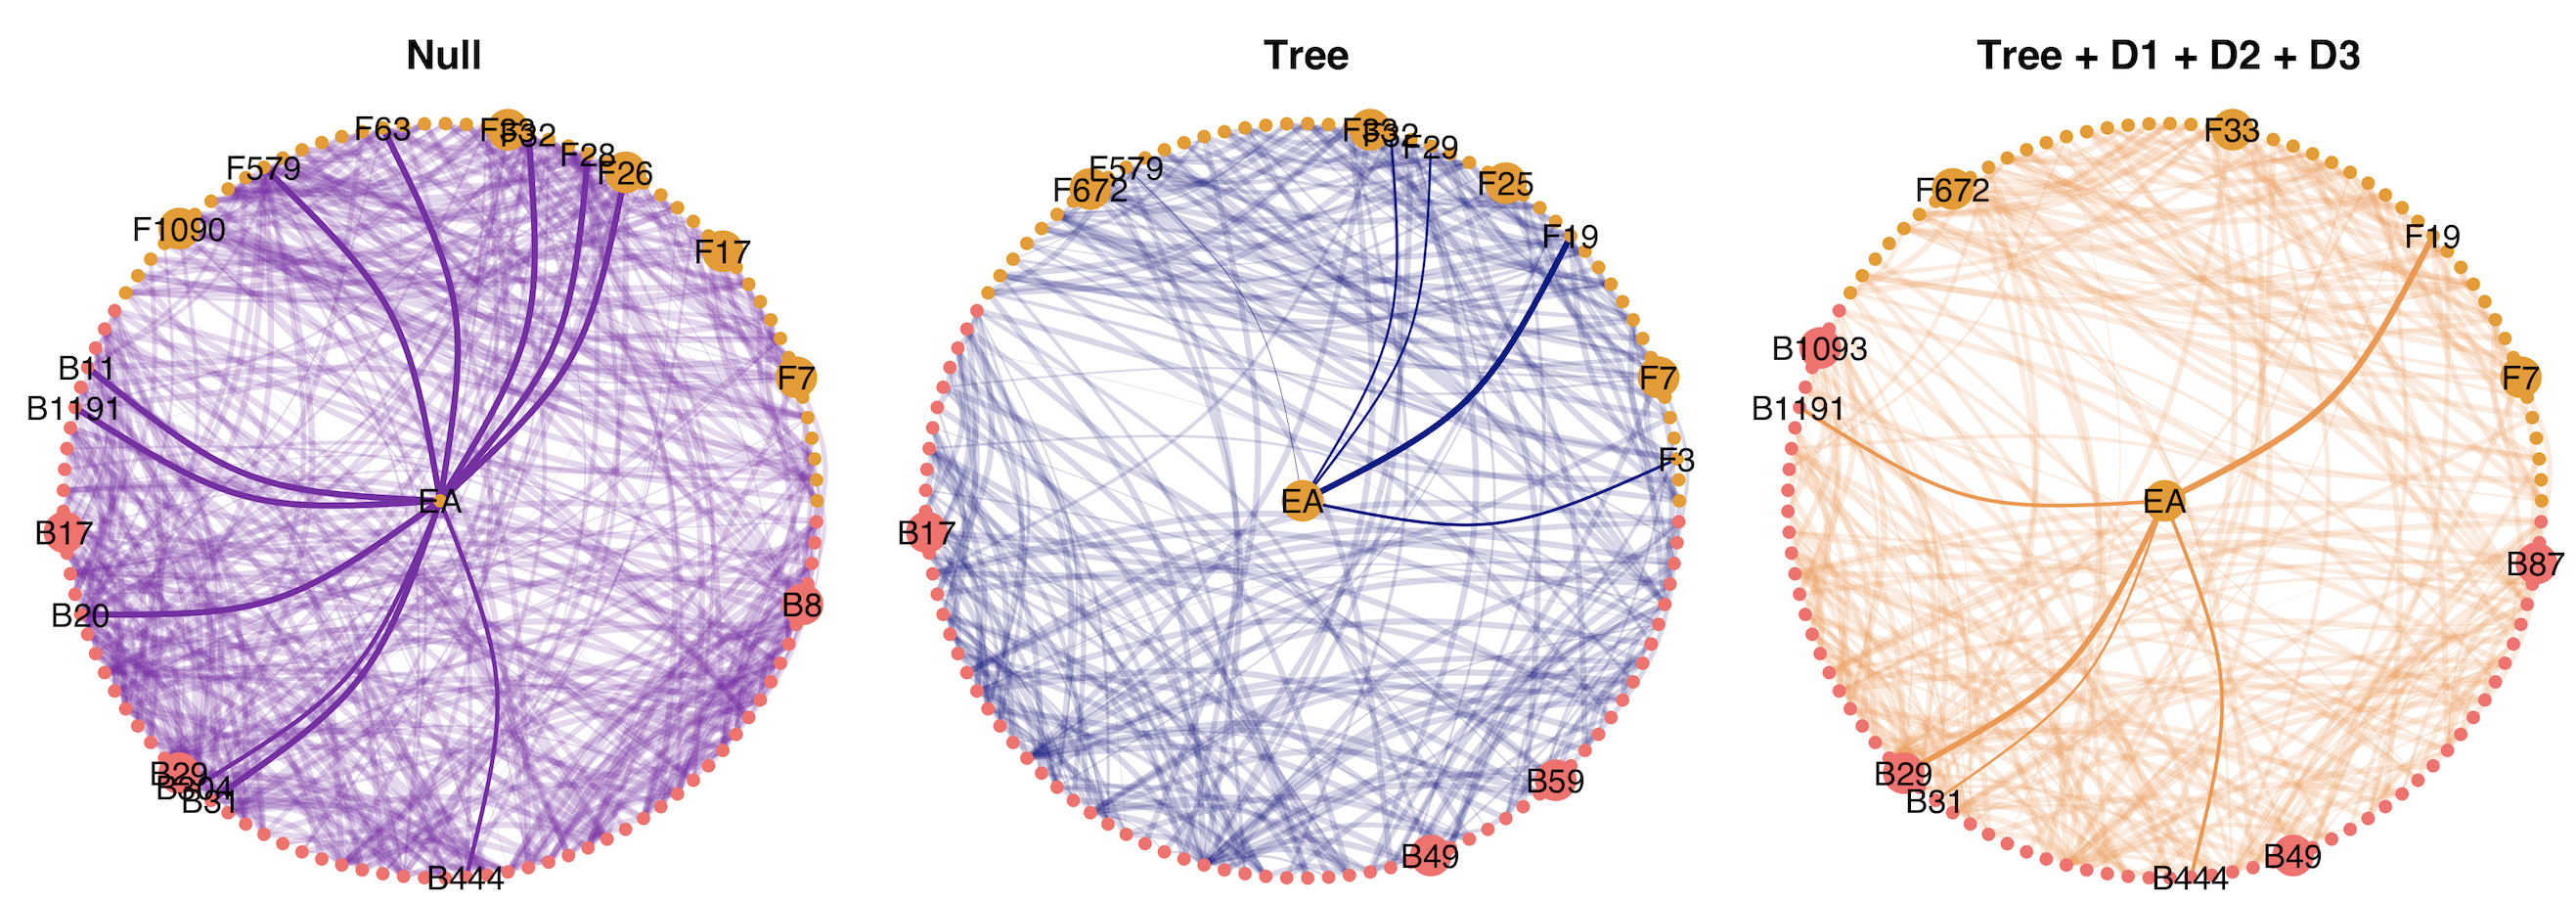
\includegraphics[width=\linewidth]{images/OakProbNets.png}
   \end{column}
   \begin{column}{0.4\linewidth}
   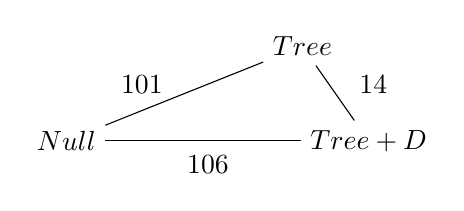
\begin{tikzpicture}	
      \tikzstyle{every edge}=[-,>=stealth',auto,thin,draw]
		\node (A1) at (0*\dist, 0*\dist) {$Null$};
		\node (A2) at (0.64*\dist, 0*\dist) {$Tree+D$};
		\node (A3) at (0.5*\dist, 0.2*\dist) {$Tree$};
	    \node (D1) at (0.16*\dist, 0.12*\dist) {$101$};
	   \node (D2) at (0.65*\dist, 0.12*\dist) {$14$};
	    \node (D3) at (0.3*\dist, -0.05*\dist) {$106$};
		\draw (A1)  edge [] (A3)
		 (A2)  edge [] (A3)
		  (A2)  edge [] (A1);
	\end{tikzpicture}  
   \end{column}
 \end{columns}
 
 \end{frame}

 \subsection{Data specificities}
 \begin{frame}{A different emission law}
  \begin{equation*}
 \left\{ \begin{array}{l}
 
 T\sim \prod_{kl\in T} \beta_{kl} / B, \\\\
 \Zbf_i\mid T  \sim \Ncal (0, \Omegab_T), \\\\
 Y_{ij}\mid \Zbf_i\sim \mathcal{F}_j (o_{ij},\xb_i,Z_{ij}).
 \end{array} \right. 
 \end{equation*}
 \bigskip
 
 $\mathcal{F}_j: \mathcal{B}, \mathcal{P}, ...$
 \end{frame}
  \begin{frame}{Account for spatial dependencies}
%\begin{description}
%\item[Mean effect] \begin{itemize}
%\item[]
%\item Spatial covariates in the model (ex: coordinates...) \end{itemize}
%\item[Variance effect]\begin{itemize}
%\item[]
%\item Spatial as a missing actor
%\item Spatial variances in the model
%\end{itemize}
%\end{description}
Separate dependencies: \emphase{$\Gamma=(\Gamma_{st})_{1\leq s,t\leq n}$}, $\Sigma_T=(\sigma_{jk})_{1\leq j,k\leq p}$.
\begin{columns}
\begin{column}{0.6\linewidth}
\begin{center}
\begin{equation*}
\left\{
\begin{array}{ll}
\Cov{(Z_{sj},Z_{sk})}& = \gamma_{ss} \sigma_{jk}\\
\Cov{(Z_{sj},Z_{tj})} &=  \sigma_{jj}\gamma_{st}
\end{array}\right.
\end{equation*}
\end{center}
\vspace{0.5cm}
\end{column}
\begin{column}{0.4\linewidth}
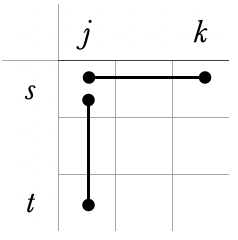
\includegraphics[width=0.4\linewidth]{images/spatial.png}
\end{column}
\end{columns}

 Defining $Vec(\Zbf) = (Z_{11},..., Z_{1p},Z_{21},...,Z_{np}) \in \mathds{R}^{n\times p}$, we obtain:
$$Vec(\Zbf) \sim \Ncal(0,\Gamma \otimes \Sigma_T).$$ 
$\Gamma$ as a function of $| s-t|$ reduces the number of parameters.
 \end{frame}
 %==============================
 \subsection{Direct network}
 \begin{frame}{Network inference from counts}
  With \emphase{any marginal and bivariate distribution for counts}:\\
\begin{columns}
 \begin{column}{0.1\linewidth}
  \begin{flushright}
	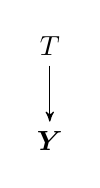
\begin{tikzpicture}	
      \tikzstyle{every edge}=[-,>=stealth',auto,thin,draw]
		\node (A1) at (0*\length, 0.8*\length) {$T$};
		\node (A3) at (0*\length, 0*\length) {$\Ybf$};
		\draw (A1)  edge [->] (A3);
	\end{tikzpicture} 
   \end{flushright}
   \end{column}
    \begin{column}{0.9\linewidth}
 $$p_\theta(\Ybf_i \mid T) = \prod_{j=1}^p p_\theta(Y_{ij}) \prod_{jk\in T} \frac{p_\theta(Y_{ij},Y_{ik})}{p_\theta(Y_{ij})p_\theta(Y_{ik})}.$$
  \end{column}
  \end{columns}
  \vspace{0.5cm}
  
The joint distribution of counts would be a mixture on spanning trees:
$$p_{\beta, \theta}(\Ybf ) = \sum_{T\in \mathcal{T}} p_\beta(T)p_\theta(\Ybf\mid T).$$

 \end{frame}
  %==============================
 \section{Simulation studies}
 \subsection{EMtree}

  %==============================
 \subsection{nestor}
 \begin{frame}{Reconstruction of the missing actor}
  \begin{figure}
 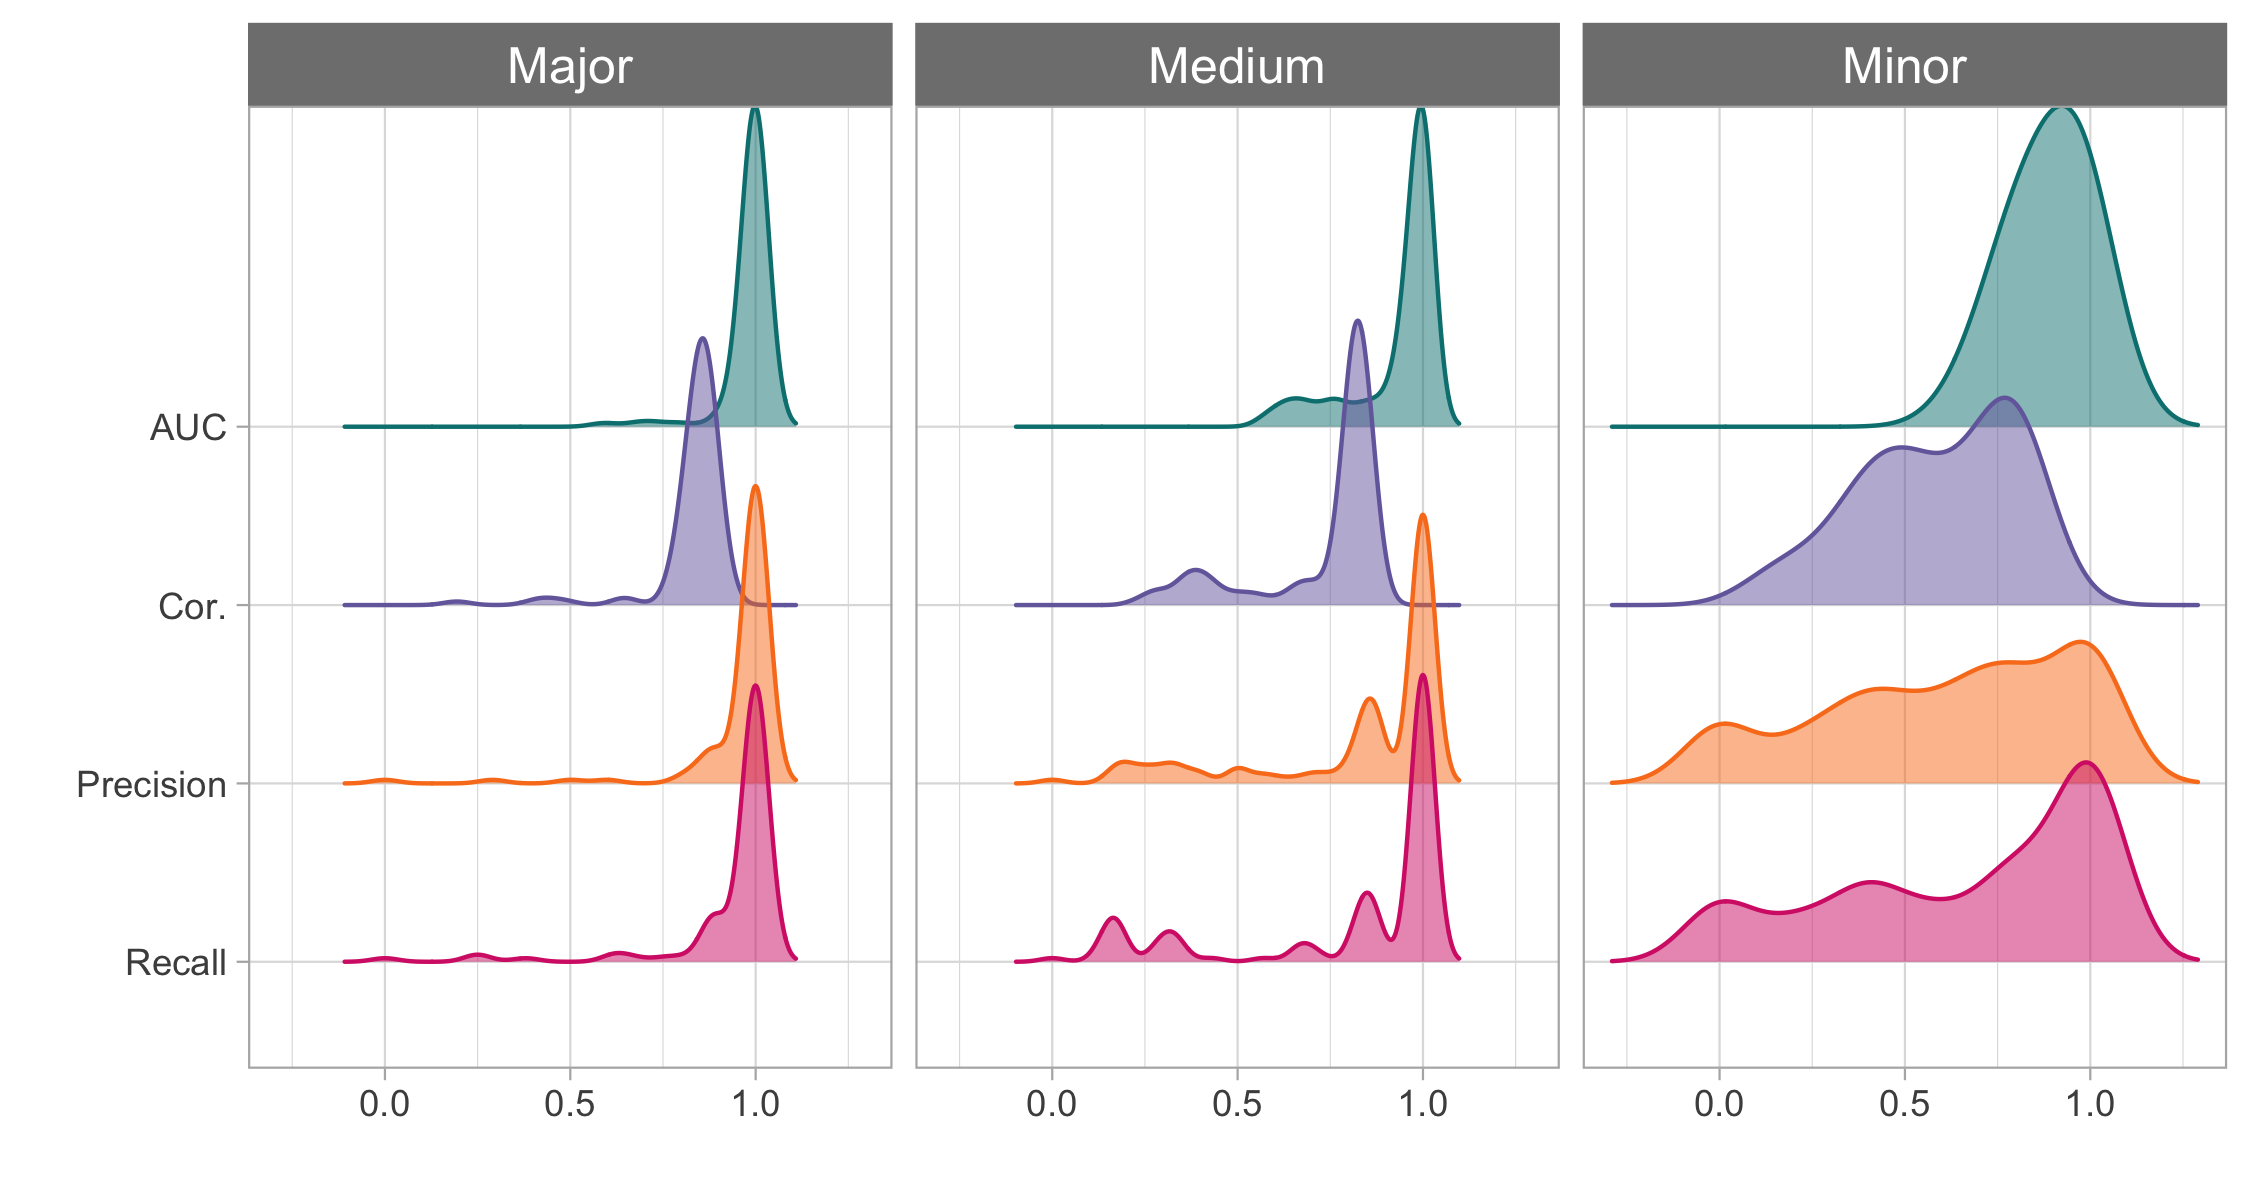
\includegraphics[width=0.9\linewidth]{images/simu_densities.png}
 \end{figure}
 \end{frame}
  %==============================
  \begin{frame}{Initialize with more potential neighbors}
  \begin{figure}
 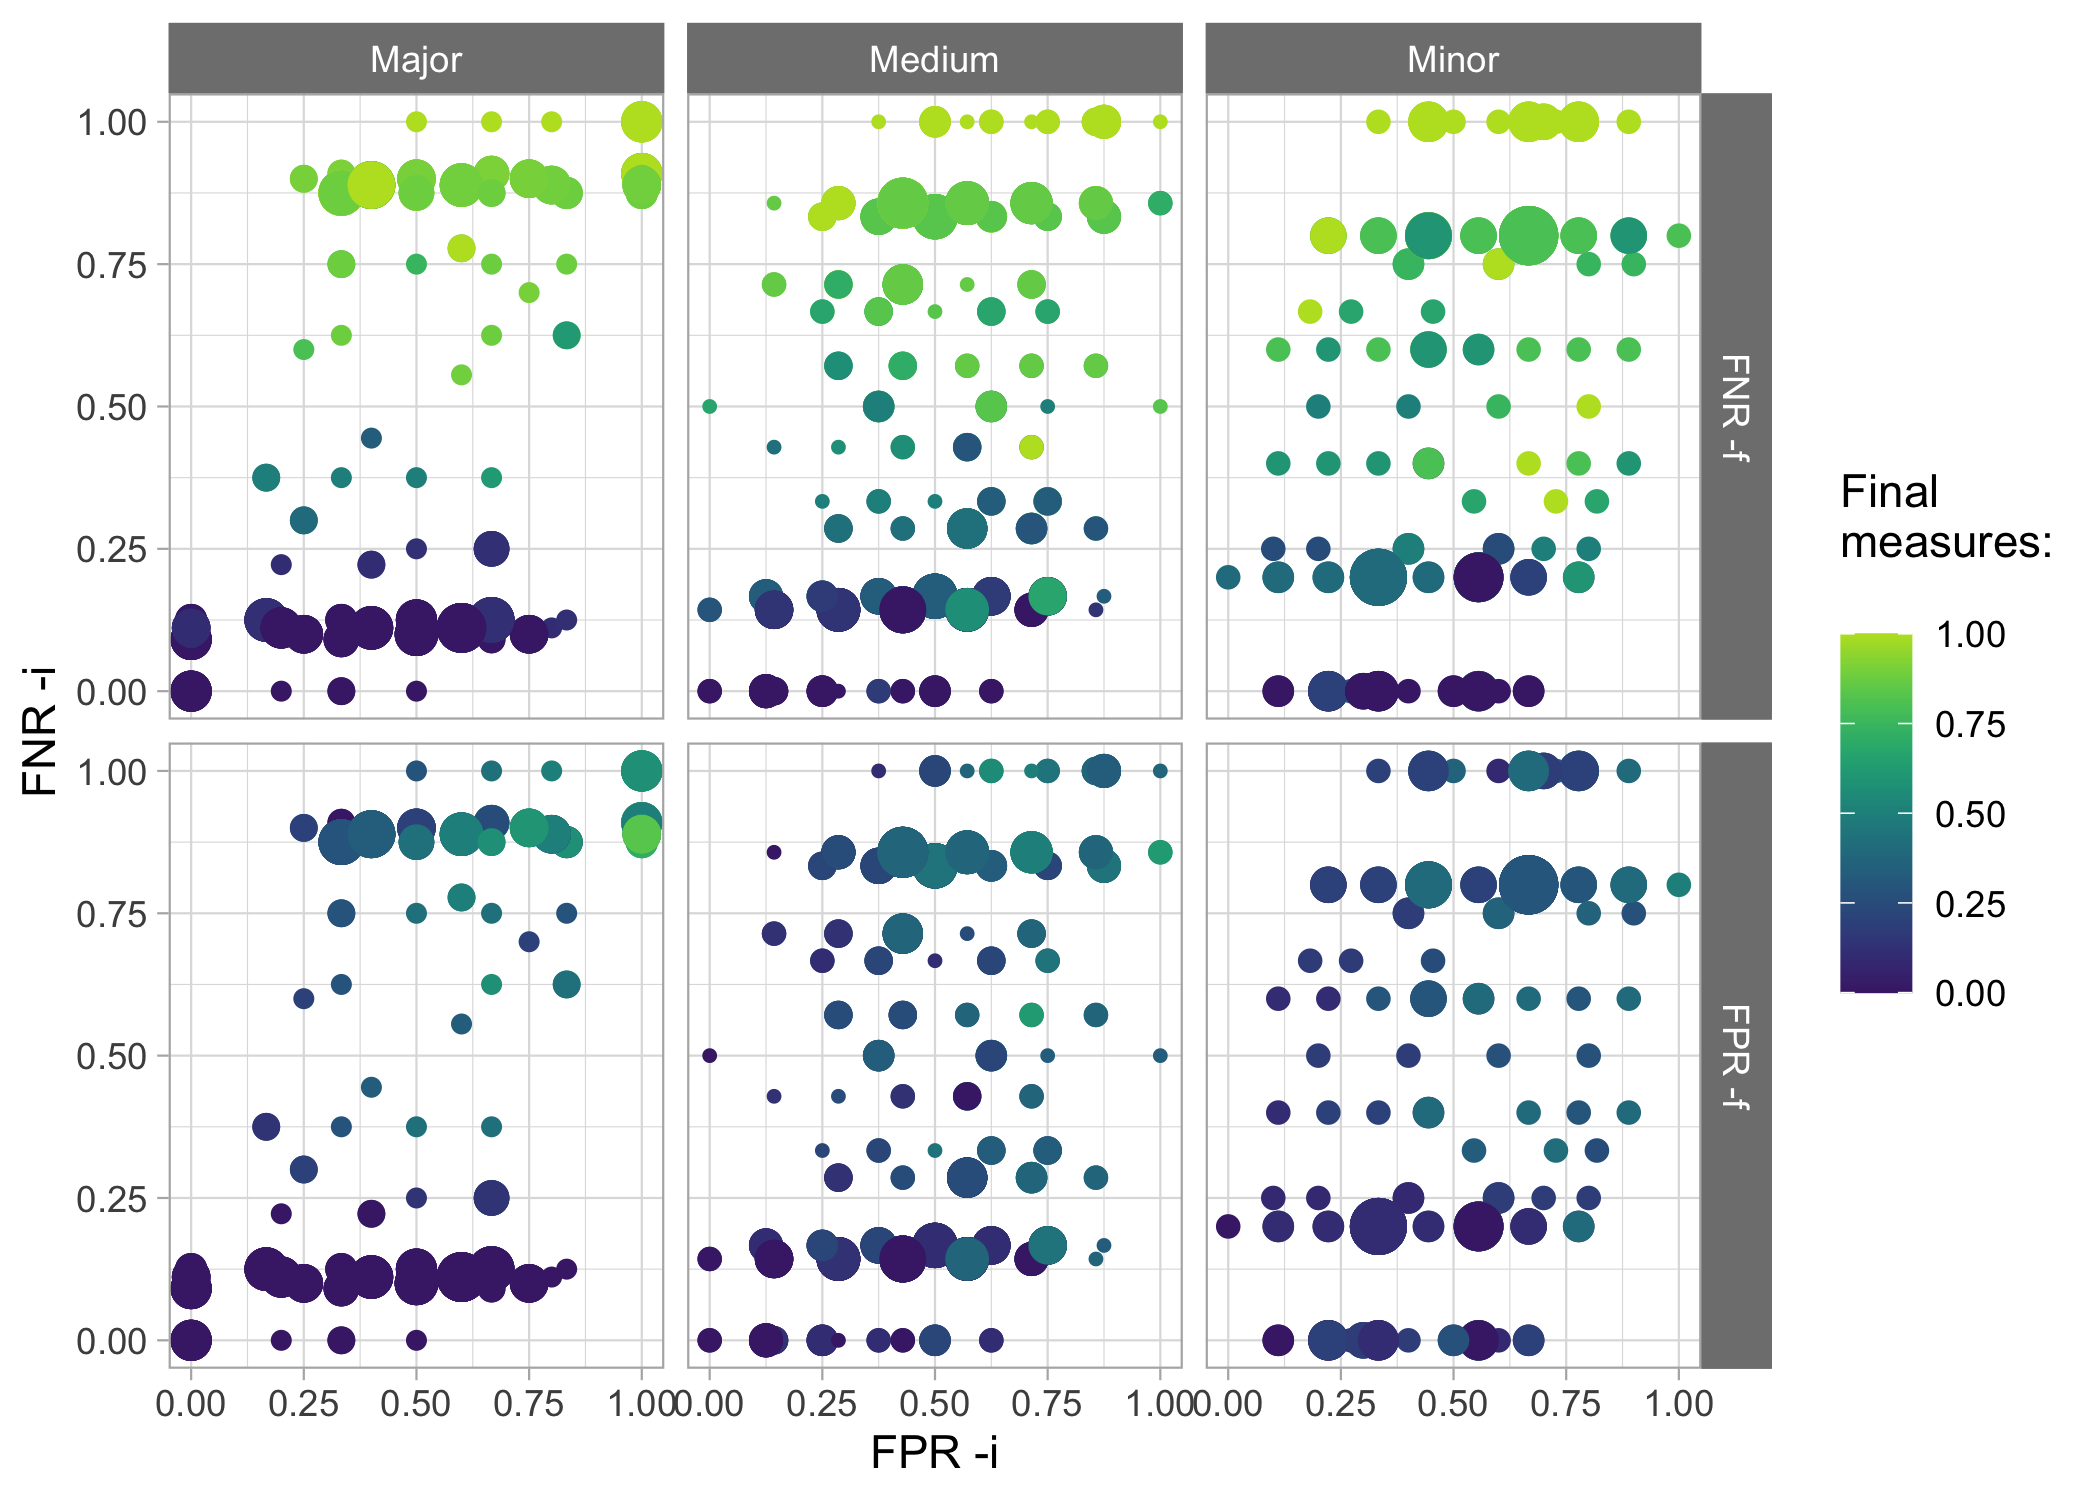
\includegraphics[width=0.8\linewidth]{images/quali_init_spca.png}
 \end{figure}
 \end{frame}
 
  %==============================
  
 \section{Miscellaneous}
 \begin{frame}{Lauritzen's notation}
 For any square matrix $\Abf$:
  $$([\Abf_B]^p )_{ij}=\left\{ \begin{array}{rl}
a_{ij} & \text{if } \{i,j\}\in B,\\
0 &  \text{if } \{i,j\}\notin  B.
\end{array}\right.$$

\bigskip 

$$\Abf=\left(\begin{array}{lll}
*&*&*\\
*&*&*\\
*&*&*
\end{array}\right) \;\;\;\Rightarrow\;\;\; [\Abf_{\{2,3\}}]^3=\left(\begin{array}{lll}
0&*&*\\
0&*&*\\
0&0&0
\end{array}\right) $$
 \end{frame}
  %==============================
  
 \begin{frame}{The M matrix}
 \begin{block}{Lemma \citep{MeilaJaak}}
 $\Qb^{pp}$ is the Laplacian matrix $\Qb$ to which the the last column and row were removed. M is then defined as follows:
 
  \begin{equation*}
  [M]_{jk}=  \left\{\begin{array}{ll}
 [(\Qb^{pp})^{-1}]_{jj} + [(\Qb^{pp})^{-1}]_{kk}-2 [(\Qb^{pp})^{-1}]_{jk}
 & 1\leq j, k <p  \\
 
 [(\Qb^{pp})^{-1}]_{jj}& k=p, 1\leq j < p\\  
 
  0 & k=j\\
 \end{array}   \right.
 \end{equation*}
 \end{block}
 
 \end{frame}
 
  %==============================
  
  \begin{frame}{Prevent numerical issues}
The Laplacian matrix $\Qb$ must be positive definite, which calls for some numerical control of the weights $\beta$:
\begin{itemize}
\item centering in log scale
\item sum constraint 
\end{itemize}
\bigskip

  Variational weights depend on the number of available samples $n$. Tempering parameter $\alpha$:
   $$\log \widetilde{\beta}_{kl} = \log \beta_{kl} - \emphase{\alpha}(\frac{n}{2}\log|\widehat{\Rbf}_{Tkl}| + \widehat{\omega}_{Tkl} [M^\intercal M]_{kl}).$$
   
  \end{frame}
%\subsection{Simulation study}
%\begin{frame}{Simulation design}
%
%\begin{enumerate}
%     \item Choose  \emphase{$G$} and randomly define the sign of its entries
%     \item build \emphase{$\Omega_G = Q(G) + \delta\times \text{I}$}, positive definite and   \emphase{$\Sigma_G = \Omega_G^{-1}$} accordingly
%     \item Sample count data \emphase{$Y$} from $\mathcal{P\ell N}(X,\Sigma_G)$ with $X$ a quantitative covariate matrix
%     \item Infer the networks with all methods
%     \item Compare results with  presence/absence of edges (\emphase{FDR}, \emphase{AUC})
%\end{enumerate}
%
%\end{frame}
%
%\begin{frame}{Questions}
%What are the effects of 
%\bigskip
%\begin{itemize}
%\item  the \emphase{graph type} of structure (Erdös-Reyni, cluster, scale-free),
%\item  the data \emphase{dimensions} (number of samples/species),
%\item  the graph edge \emphase{density}\\
%\end{itemize}
%\bigskip
%
%on the methods performance ?
%\end{frame}

%====================================================================
%\begin{frame}{Data dimensions: Erdös results}
%\bleu{False Discovery Rate (FDR):} how many false edges  among those detected?\\
%\bleu{Density ratio:} (\# detections) /  (\# true edges)
%
%\begin{figure}
%    \centering
%       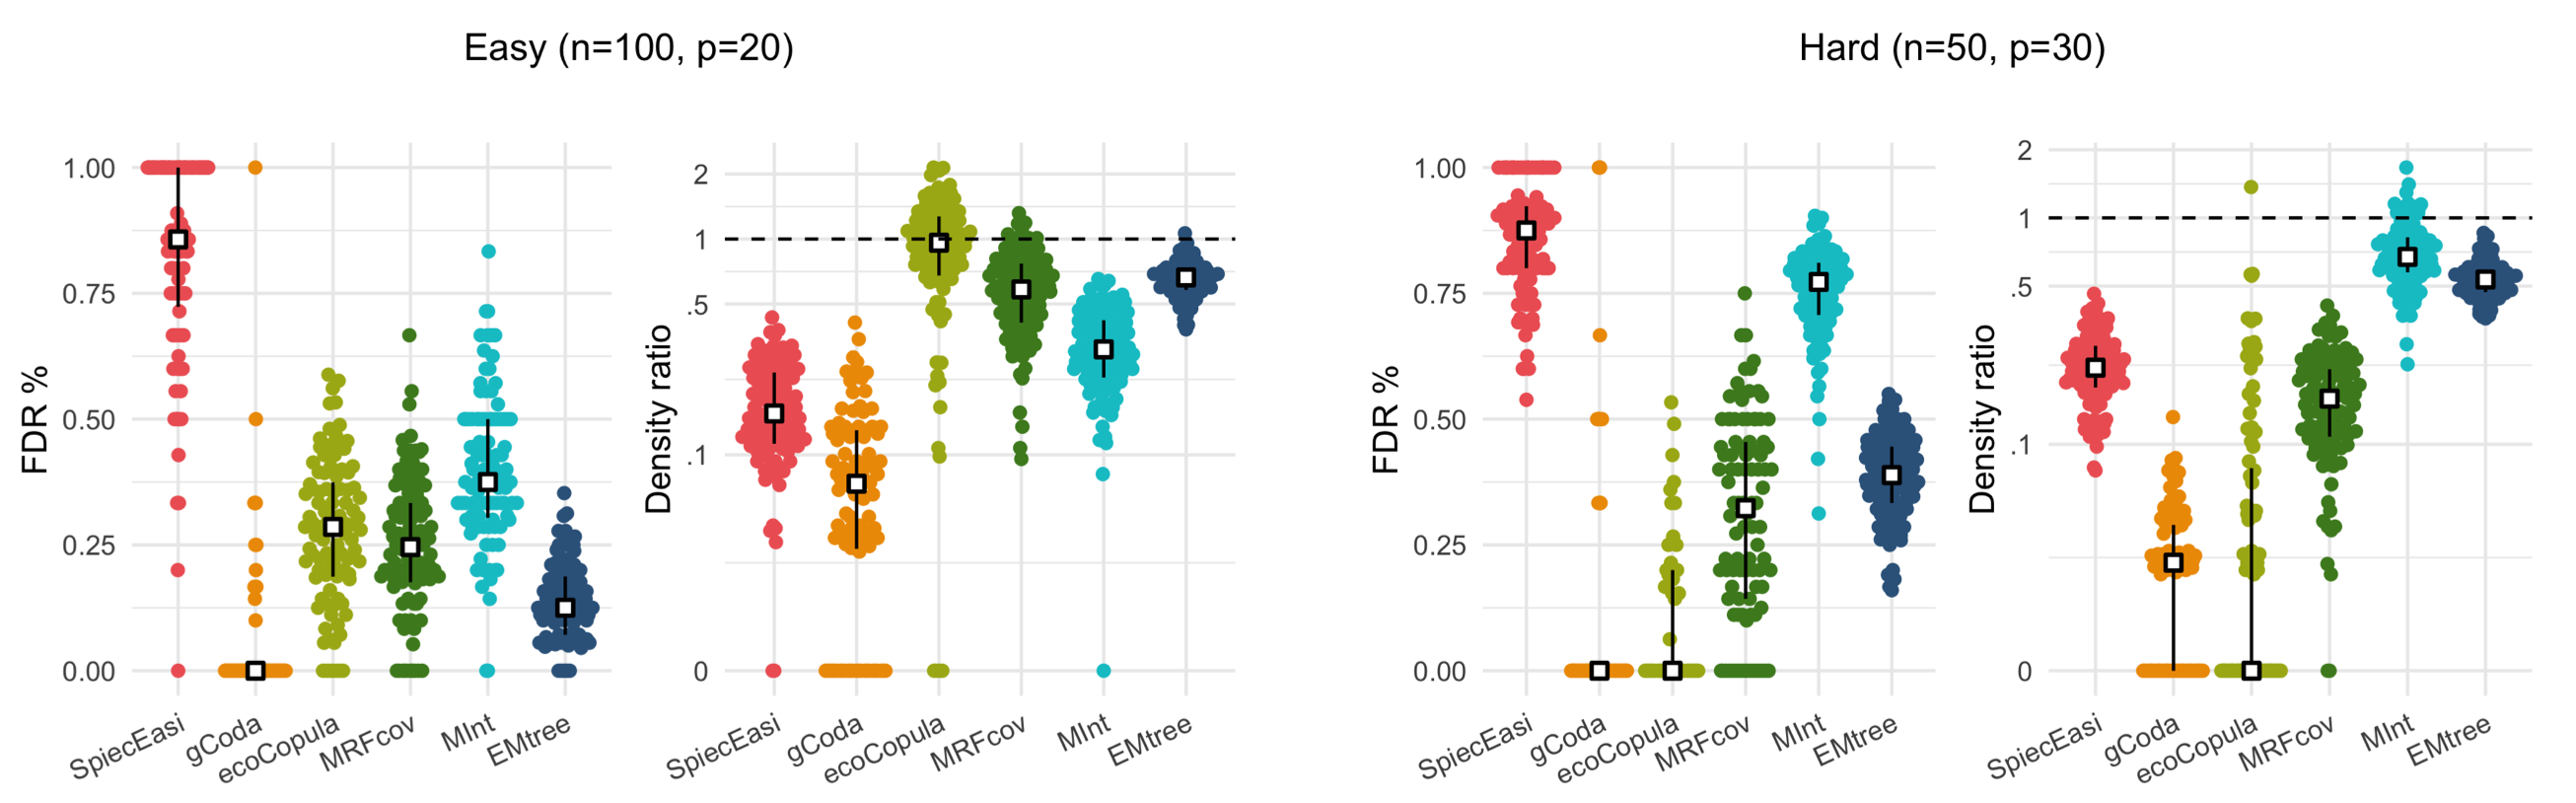
\includegraphics[width=\linewidth]{images/panel_erdos_6methods.png} 
%\end{figure}
%\begin{itemize}
%    \item EMtree: the smallest FDR with a reasonable density ratio
%    \item $20\%$ increase in FDR when the difficulty level increases
%\end{itemize}
%\end{frame}
%====================================================================

%\begin{frame}{Data dimensions: running times}
%
%\scriptsize
%\begin{table}
%\begin{tabular}{l|rrrrrr}
% & \multicolumn{1}{c}{SpiecEasi} & \multicolumn{1}{c}{gCoda} & \multicolumn{1}{c}{ecoCopula} & \multicolumn{1}{c}{MRFcov} & \multicolumn{1}{c}{MInt} & \multicolumn{1}{c}{EMtree} \\ 
%  \hline
%Easy &  19.99(4.19) & 0.1(0.05) & 4.2(0.24) & 5.76(0.35) & 54(26.9) & 4.44(0.64) \\ 
%  Hard &  24.29(5.07) & 0.5(0.24) & 8.19(0.16) & 5.52(2.98) & 33.87(18.37) & 3.29(0.32)  \\ 
%   \hline
%\end{tabular}
%\caption{Median and standard-deviation running-time values (in seconds) for Cluster and Erdös structures, including resampling with $S=20$ for SpiecEasi and EMtree.}
%\label{timesTPFN}
%\end{table}
% 
%\normalsize
%\begin{itemize}
%\item EMtree ranks $3^{rd}$/6 in easy cases and $2^{nd}$ in hard ones 
%\end{itemize}
%\end{frame}
%====================================================================

%\begin{frame}{Network density}
%\footnotesize{\bleu{Area under the (ROC) curve (AUC):} "how good is a classifier to rank true positives higher"}\\
% \begin{figure}[H]
%  \centering
%  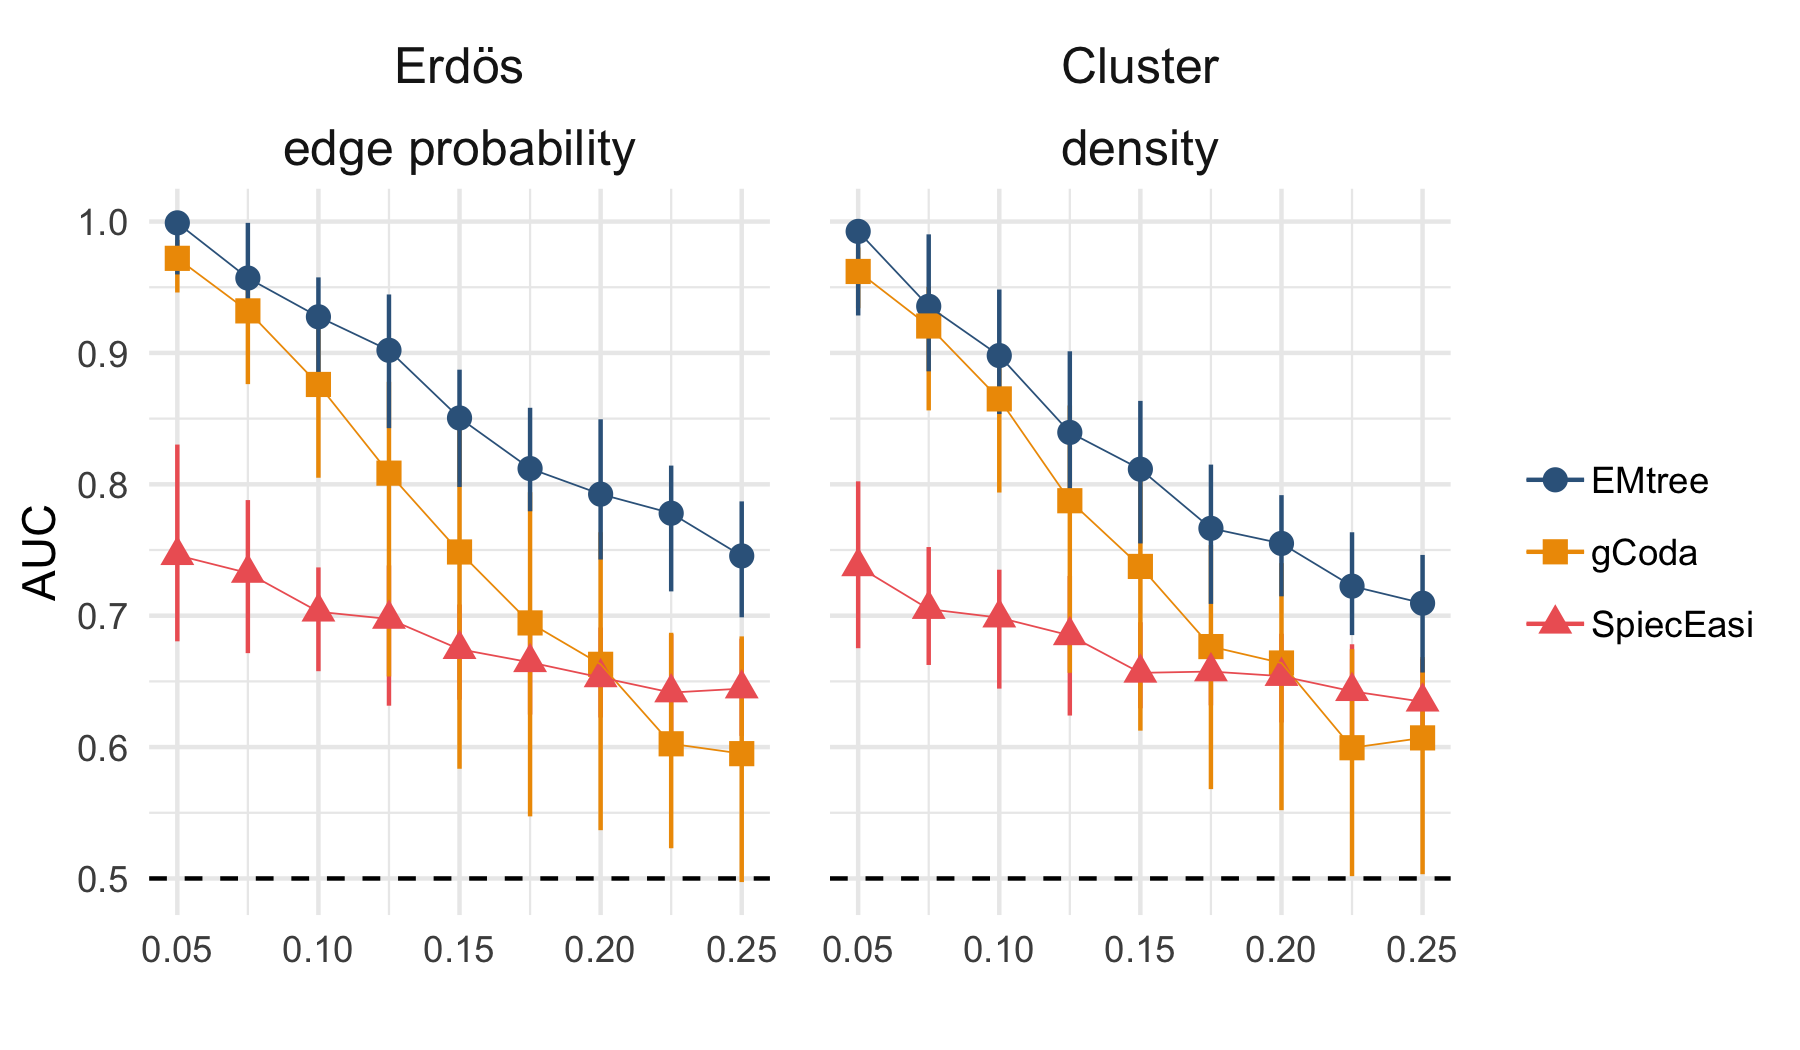
\includegraphics[width=7cm]{images/panel_dens.png}
%  \caption{\scriptsize{Effect of graph density on the evolution of AUC median and inter-quartile intervals in Erdös and Cluster structures. (100 observations, 20 species)}}
%\end{figure}
%\normalsize
%$\Rightarrow$ The tree assumption does not alter the performance
%\end{frame}
\backupend



\end{document}